%!TEX root = ../thesis.tex
\externaldocument[A-]{Chapters/appendix.tex}

\part{Muxmon experiment}

  \chapter{Challenges in scaling up}
    \label{ch:Challenges in scaling up}

    \section{Frequency re-use}
      \label{sec:frequency re-use}

      \begin{wrapfigure}[16]{r}{0.45\textwidth}
        \begin{center}
        \vspace{-30pt}
          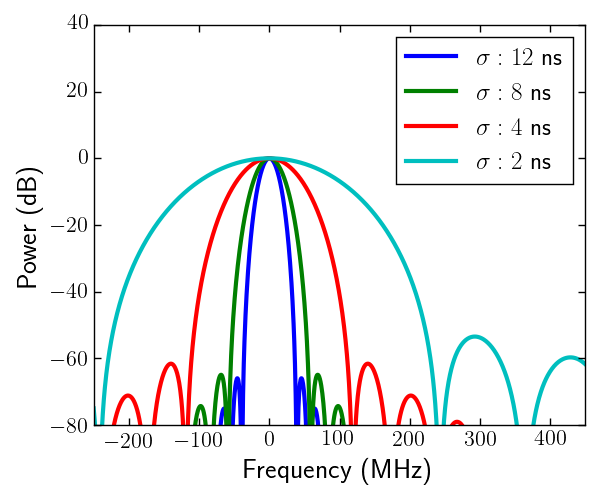
\includegraphics[width=\textwidth]{../Figures/Exploring frequency re-use/bandwidth_broadening.png}
        \end{center}
        \caption{The frequency bandwidth corresponding to Gaussian pulses with different widths $\sigma$.}
        \label{fig:bandwidth broadening}
        \vspace{-20pt}
      \end{wrapfigure}

      Even in large-scale quantum circuits individual qubit control is required. When multiple qubits are connected to a single drive line, being able to control the qubits individually requires their frequencies to be sufficiently separated. The amount by which the frequencies must be separated depends on the length of the pulses applied to the qubit. The shorter the pulse, the larger its corresponding frequency bandwidth, as can be seen in Figure~\ref{fig:bandwidth broadening}. Longer pulses, on the other hand, result in less operations being possible within the decoherence times of the qubit. It is therefore desirable to have pulses with a short duration. This means that the separation between qubit frequencies must be large. Since there is only a finite frequency spectrum, having many qubits, each with a different frequency, results in frequency crowding.

      If the qubits are not connected to the same drive line, they can be individually controlled, even when they share the same frequency. This concept is known as frequency re-use, and is a possible way to overcome frequency crowding. Frequency re-use can be implemented in the surface code architecture. One possible implementation of frequency re-use in the surface code is shown in Figure~\ref{fig:surface code frequency re-use}, where every resonator is connected to four qubits. In this set-up four distinct frequencies suffice to enable individual driving of every qubit on the lattice.

      \begin{figure}[h]
        \centering
        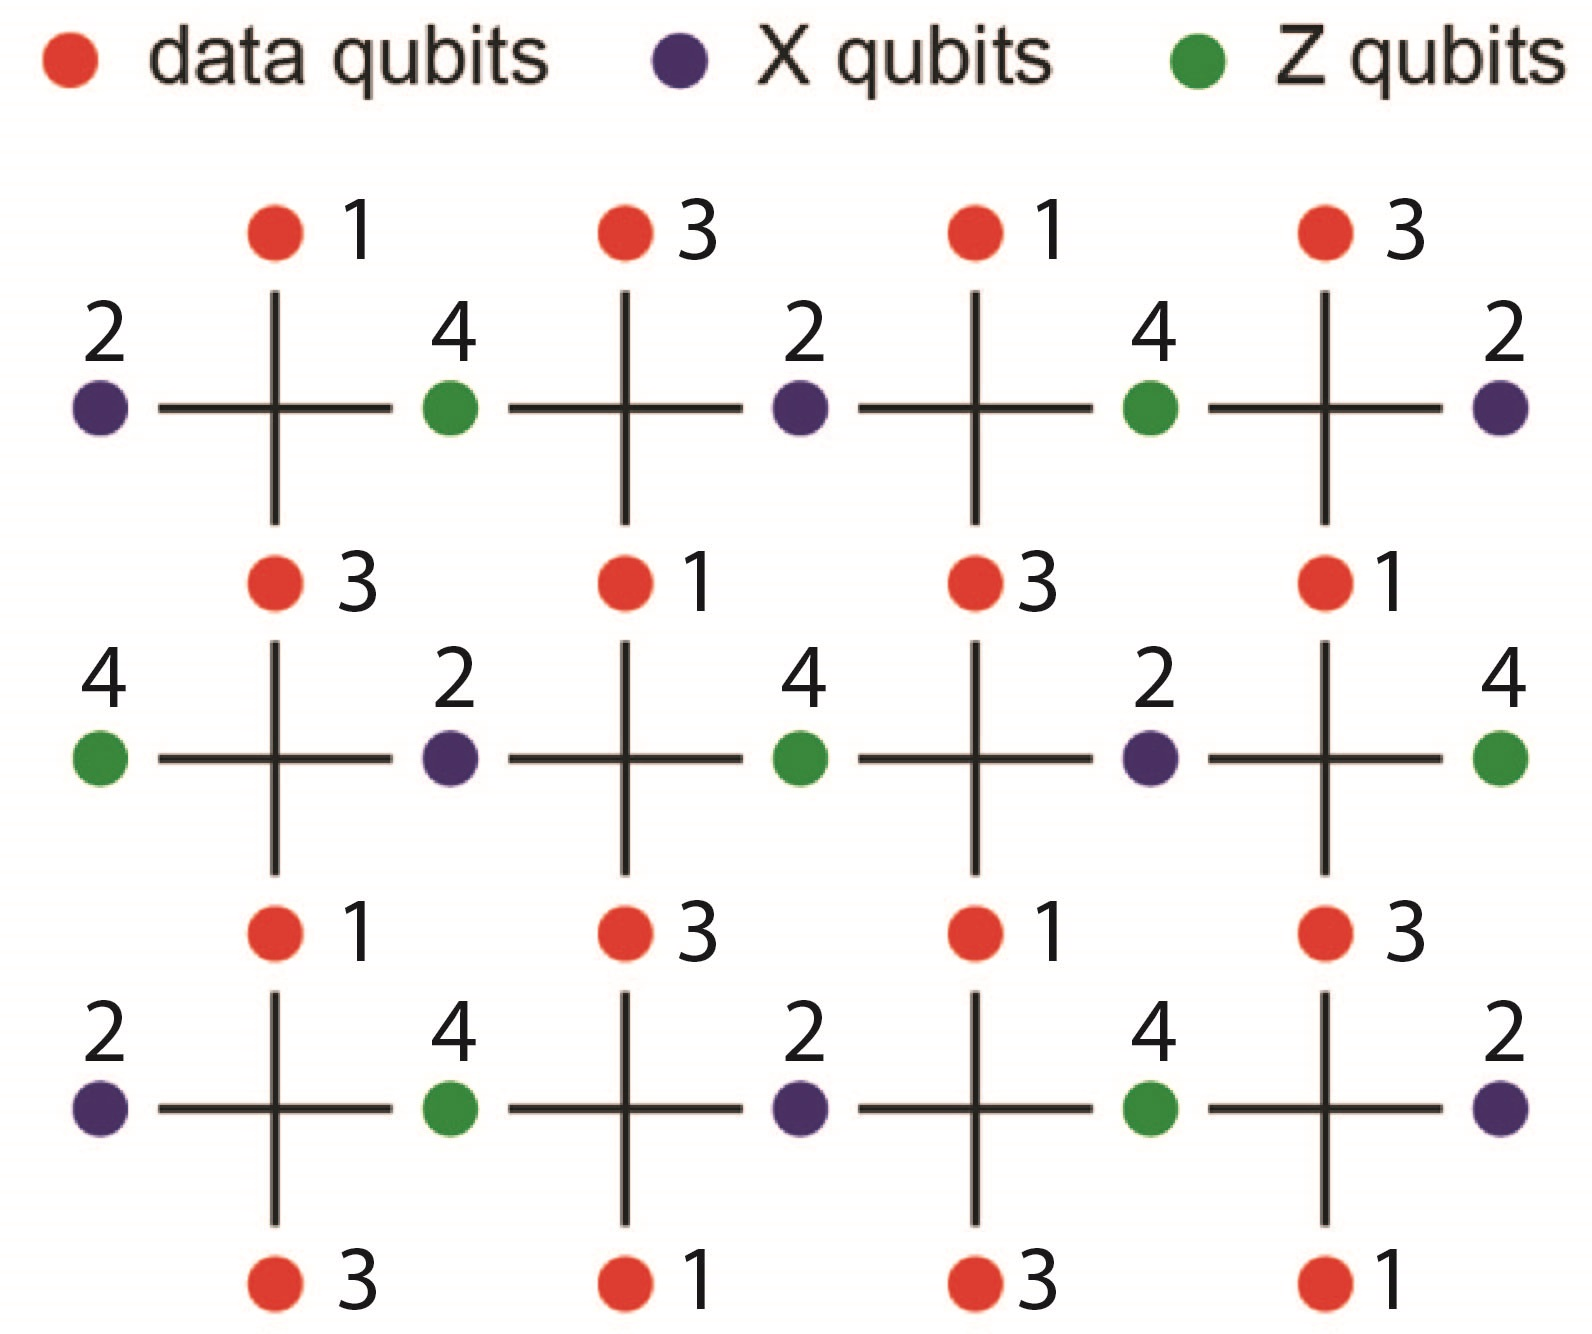
\includegraphics[width=.6\textwidth]{../Figures/Exploring frequency re-use/surface_code_frequency re-use_cut.jpg}
        \caption{A surface code architecture with the implementation of frequency re-use. The different digits correspond to distinct frequencies. }
        \label{fig:surface code frequency re-use}
      \end{figure}

      Frequency re-use does pose potential issues. Two unwanted effects in particular arise when multiple qubits that are directly or indirectly coupled to each other share the same frequency. The first effect is cross-coupling, where an excitation can be transferred from one qubit to the other. This will be discussed in Section~\ref{ssec:cross-coupling}. The second effect is cross-driving, where a pulse that partially leaks through the components will drive other qubits. The components separating qubits do not act as perfect filters, and so the pulse will always partially leak through. This does not pose a problem as long as the frequency of the pulse is sufficiently detuned from the frequency of the other qubits. In the case of frequency re-use, however, the frequencies of the qubits are the same, and so a pulse leaking through will result in cross-driving. This effect is discussed in Section~\ref{ssec:cross-driving}.

    \section{Selective broadcasting}
      \label{sec:selective broadcasting using the Duplexer}
      \begin{wrapfigure}[13]{r}{0.45\textwidth}
        \begin{center}
        \vspace{-30pt}
          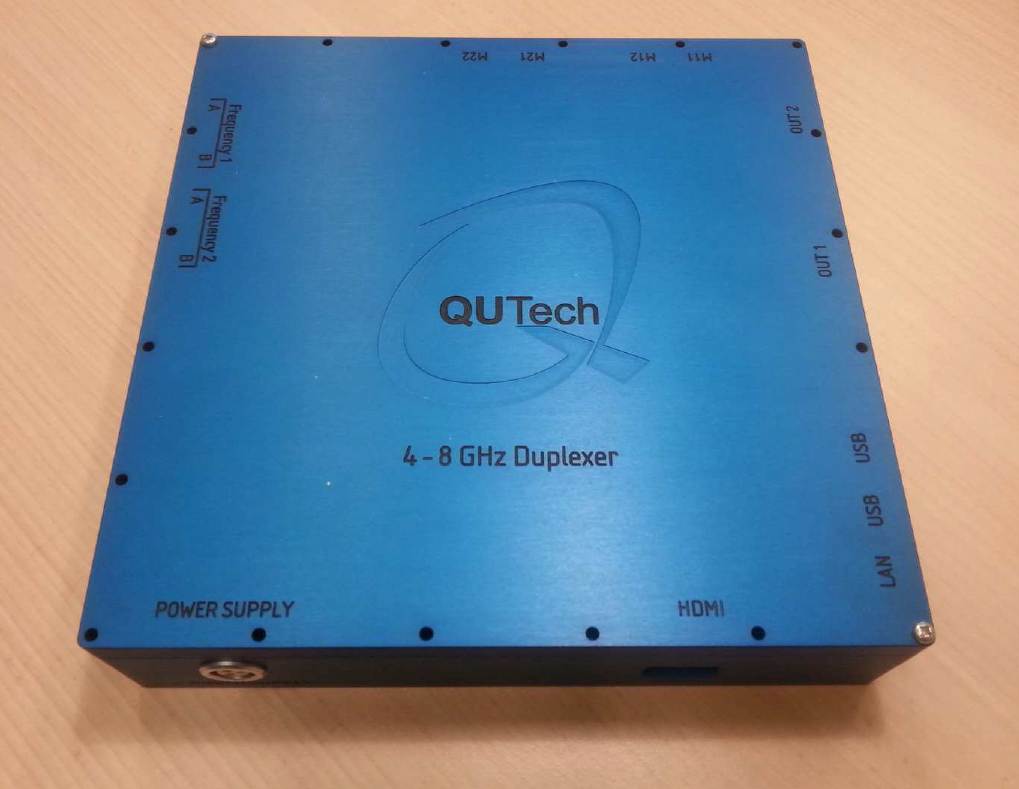
\includegraphics[width=\textwidth]{../Figures/Duplexer_with_background.png}
        \end{center}
        \vspace{-5pt}
        \caption{The Duplexer}
        \label{fig:Duplexer picture}
        \vspace{-10pt}
      \end{wrapfigure}

      A second challenge that exists when scaling up is that as the number of qubits grow, so do the instruments needed to control them. When thinking of a large-scale quantum computer, it is unrealistic to think that each qubit will have its own RF generator, AWG, and other necessary instruments. Therefore, alternatives have to be devised to combat this scaling of instruments. One such device is the Duplexer, shown in Figure~\ref{fig:Duplexer picture}. The Duplexer is a patented vector switch matrix designed by Duije Deurloo, who is working at TNO. It has four input ports and two ouput ports. Signals going through each of the input-output port combinations pass through the following successive components:

      \begin{enumerate}
        \item Digital switch
        \item Variable phase-shifter
        \item Variable attenuator
        \item Amplifier
      \end{enumerate}

      The Duplexer's digital switches have an RF-switching time of \SI{4}{\nano \second}. Using these switches, pulses may be sent to either of the two output ports, or to both output ports simultaneously. This allows for selective broadcasting, where pulses are routed to either or both of the two output ports at the nanosecond scale. When the output ports are connected to drive lines that are connected to qubits sharing the same frequency, the result is that two qubits can be controlled using a single generator and AWG. This property will be exploited in Randomized Benchmarking in Chapter~\ref{ch:randomized benchmarking}.

    \section{The Muxmon experiment}
      \label{sec: the Muxmon experiment}
      \begin{figure}[h]
      \centering
        \begin{subfigure}[b]{0.9\textwidth}
          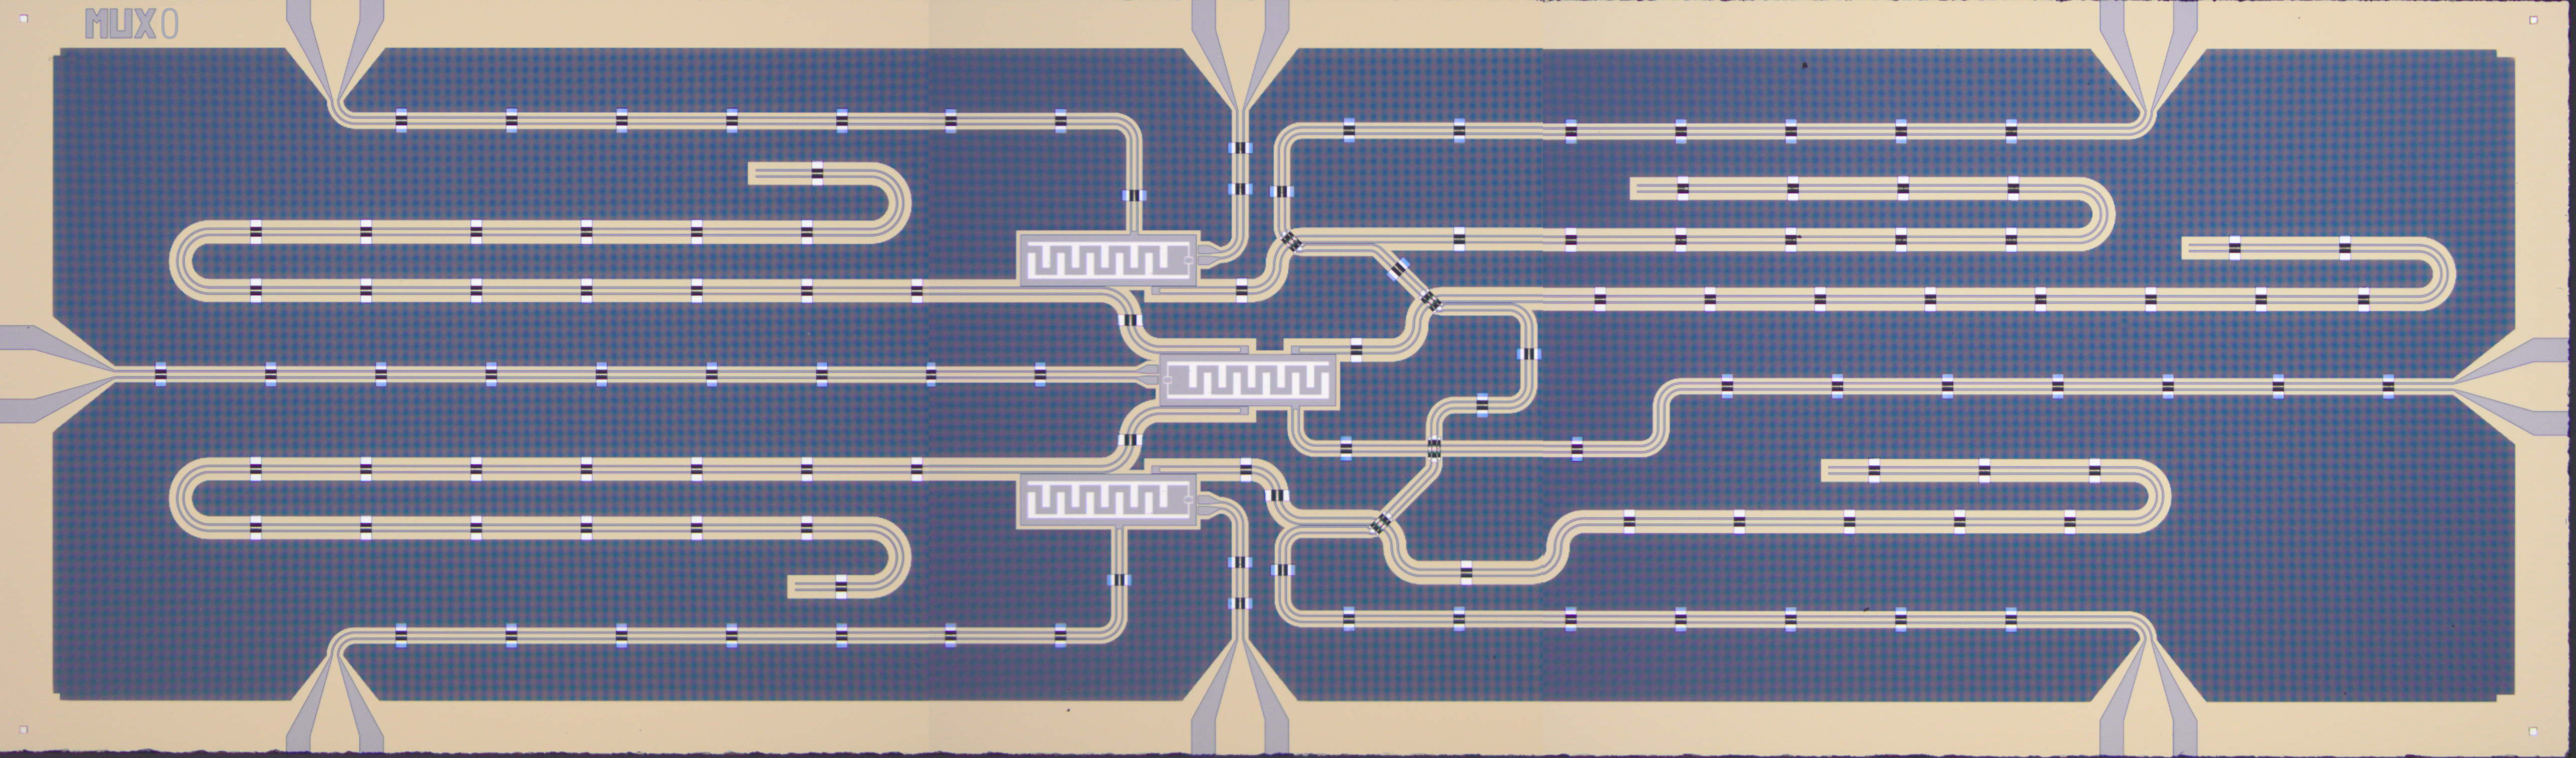
\includegraphics[width=1\linewidth]{../Figures/MUX_0.jpg}
          \caption{The Muxmon0 chip, in which the qubit drive lines are directly coupled}
          \label{fig:Muxmon0 image}
        \end{subfigure}

        \begin{subfigure}[b]{0.9\textwidth}
          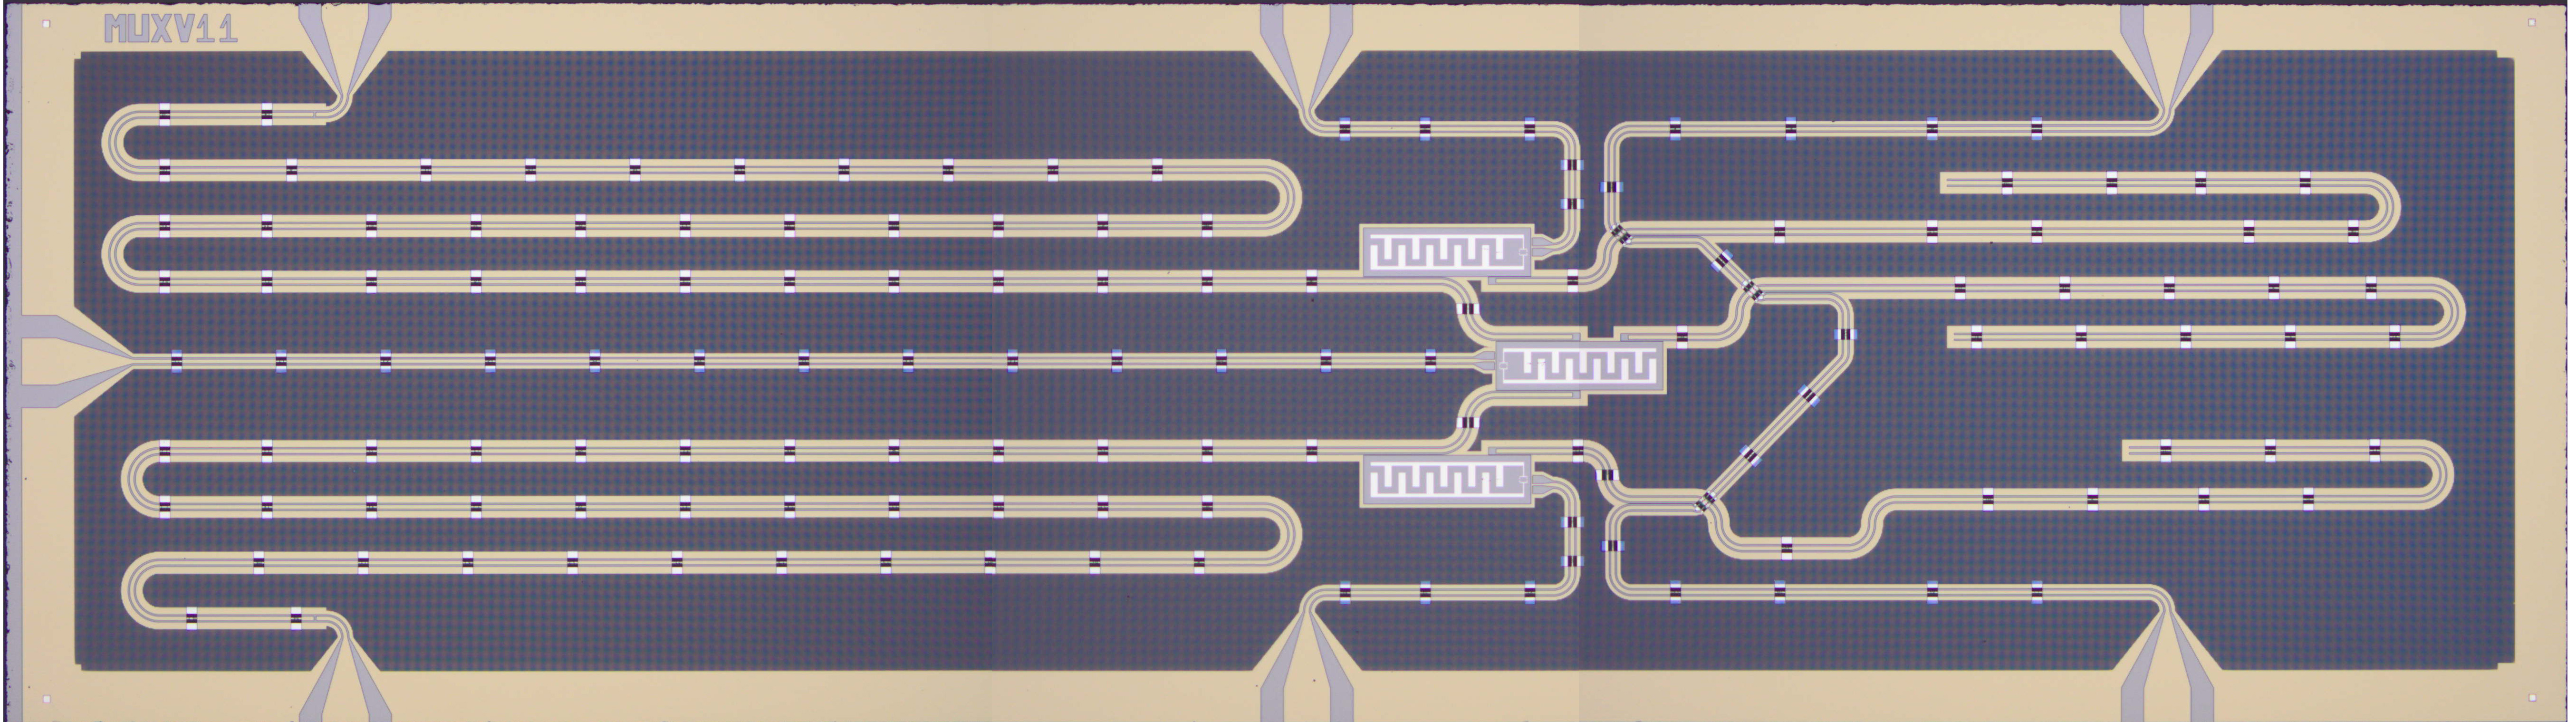
\includegraphics[width=1\linewidth]{../Figures/MUX_1.jpg}
          \caption{The Muxmon1 chip, in which the qubit drive lines are capacitively coupled}
          \label{fig:Muxmon1 image}
        \end{subfigure}
        \caption[Muxmon chips]{The Muxmon0 and Muxmon1 chips. The qubits of Muxmon0 have direct drive lines, while the qubits of Muxmon1 have drive lines capacitively coupled to the resonator buses.}
        \label{fig:Muxmon0 and Muxmon1}
      \end{figure}

      \begin{wrapfigure}[7]{r}{0.3\textwidth}
        \begin{center}
        \vspace{-30pt}
          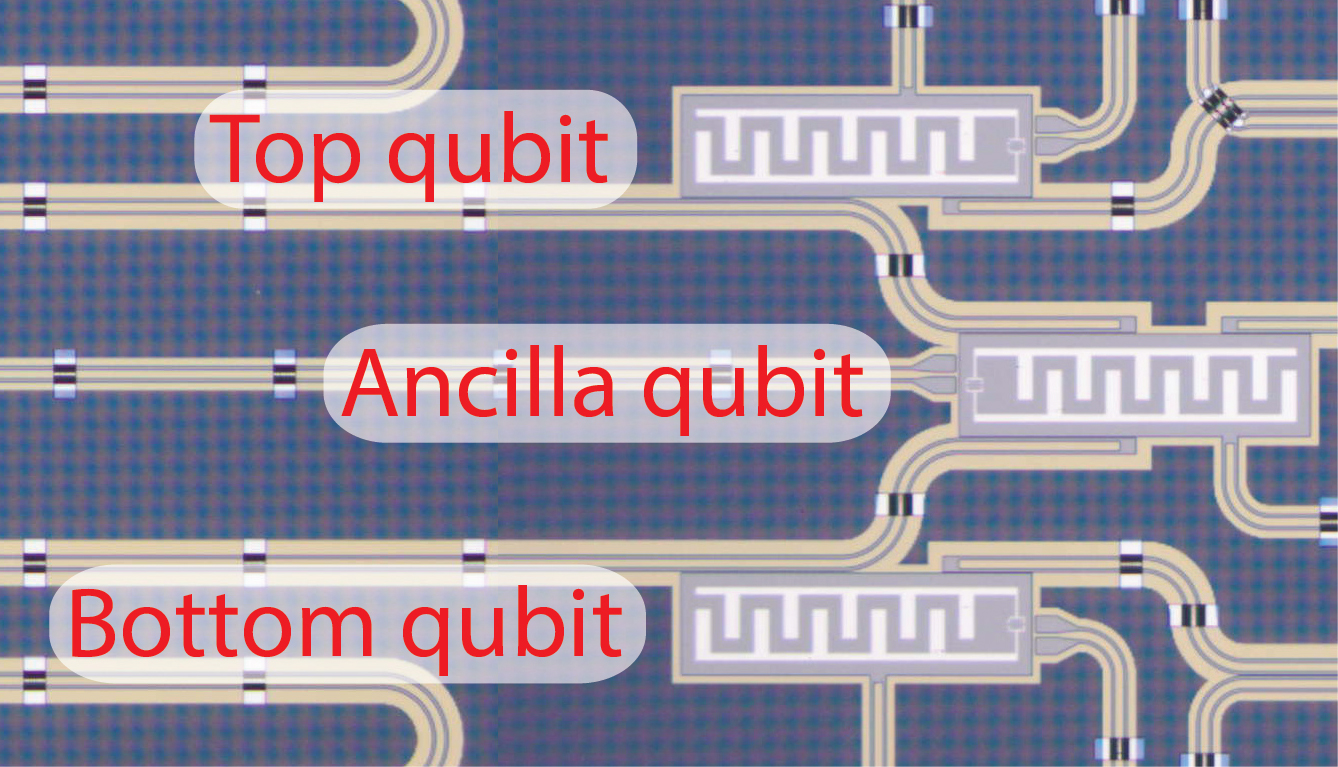
\includegraphics[width=\textwidth]{../Figures/Qubit names.jpg}
        \end{center}
        \vspace{-20 pt}
        \caption{Naming of the three qubits.}
        \label{fig:Qubit names}
      \end{wrapfigure}

      The Muxmon experiment was performed specifically to study frequency re-use and selective broadcasting using the Duplexer. Two chips were designed, Muxmon0 and Muxmon1, shown in Figure~\ref{fig:Muxmon0 and Muxmon1}. Both chips have three transmon qubits connected to them, all three of which are flux-tunable. For convenience, these qubits are named top, ancilla, and bottom qubit, as shown in Figure~\ref{Qubit names}. Air-bridges are used, not only to connect the ground-planes in the coplanar waveguides, but also such that the feedline can cross over other lines. The key difference between the two chips is the approach used to drive the qubits. In Muxmon0 all three qubits have their individual directly coupled drive lines. The top and bottom qubit are connected to the ancilla qubit through a bus. In the Muxmon1 the bus and drive lines are combined into two drive lines, each of which is capacitively coupled to the ancilla qubit and one of the other two qubits. The disadvantage of the direct drive lines in Muxmon0 is that they are an added decoherence channel for the qubits. However, the three drive lines of Muxmon0 ensure that individual qubit control of all three qubits is possible, even when they share the same frequency. This is in contrast to Muxmon1, where the ancilla qubit frequency must differ from that of the other two qubits. In the frequency re-use structure of the surface code, as explained in section~\ref{sec:frequency re-use}, this should not be a problem, as frequency re-use in not applied to neighbouring qubits. Having capacitively coupled drive lines would result in less lines being required, both on-chip and outside the chip. Furthermore there would be one decoherence channel less. Therefore the capacitive coupled drive lines of Muxmon1 seemed the more attractive of the two options.

      During initial characterization of the qubits on both chips it was found that the decoherence times of the qubits in Muxmon1 were considerably worse than those in Muxmon0 (see Appendix~\ref{sec:Muxmon1 decoherence times}. It is, however, unlikely that this is due to the capacitively coupled drive lines, since one would expect the absence of direct drive lines to result in one less decoherence channel. Instead it is likely that the lower decoherence times are simply due to some error in the chip fabrication process. Due to the lower decoherence times of the qubits in Muxmon1, the focus of the experiment was on Muxmon0. Therefore, unless states otherwise, the Muxmon chip used in the experiment refers to the Muxmon0 chip.

      \begin{figure}[tb]
        \centering
        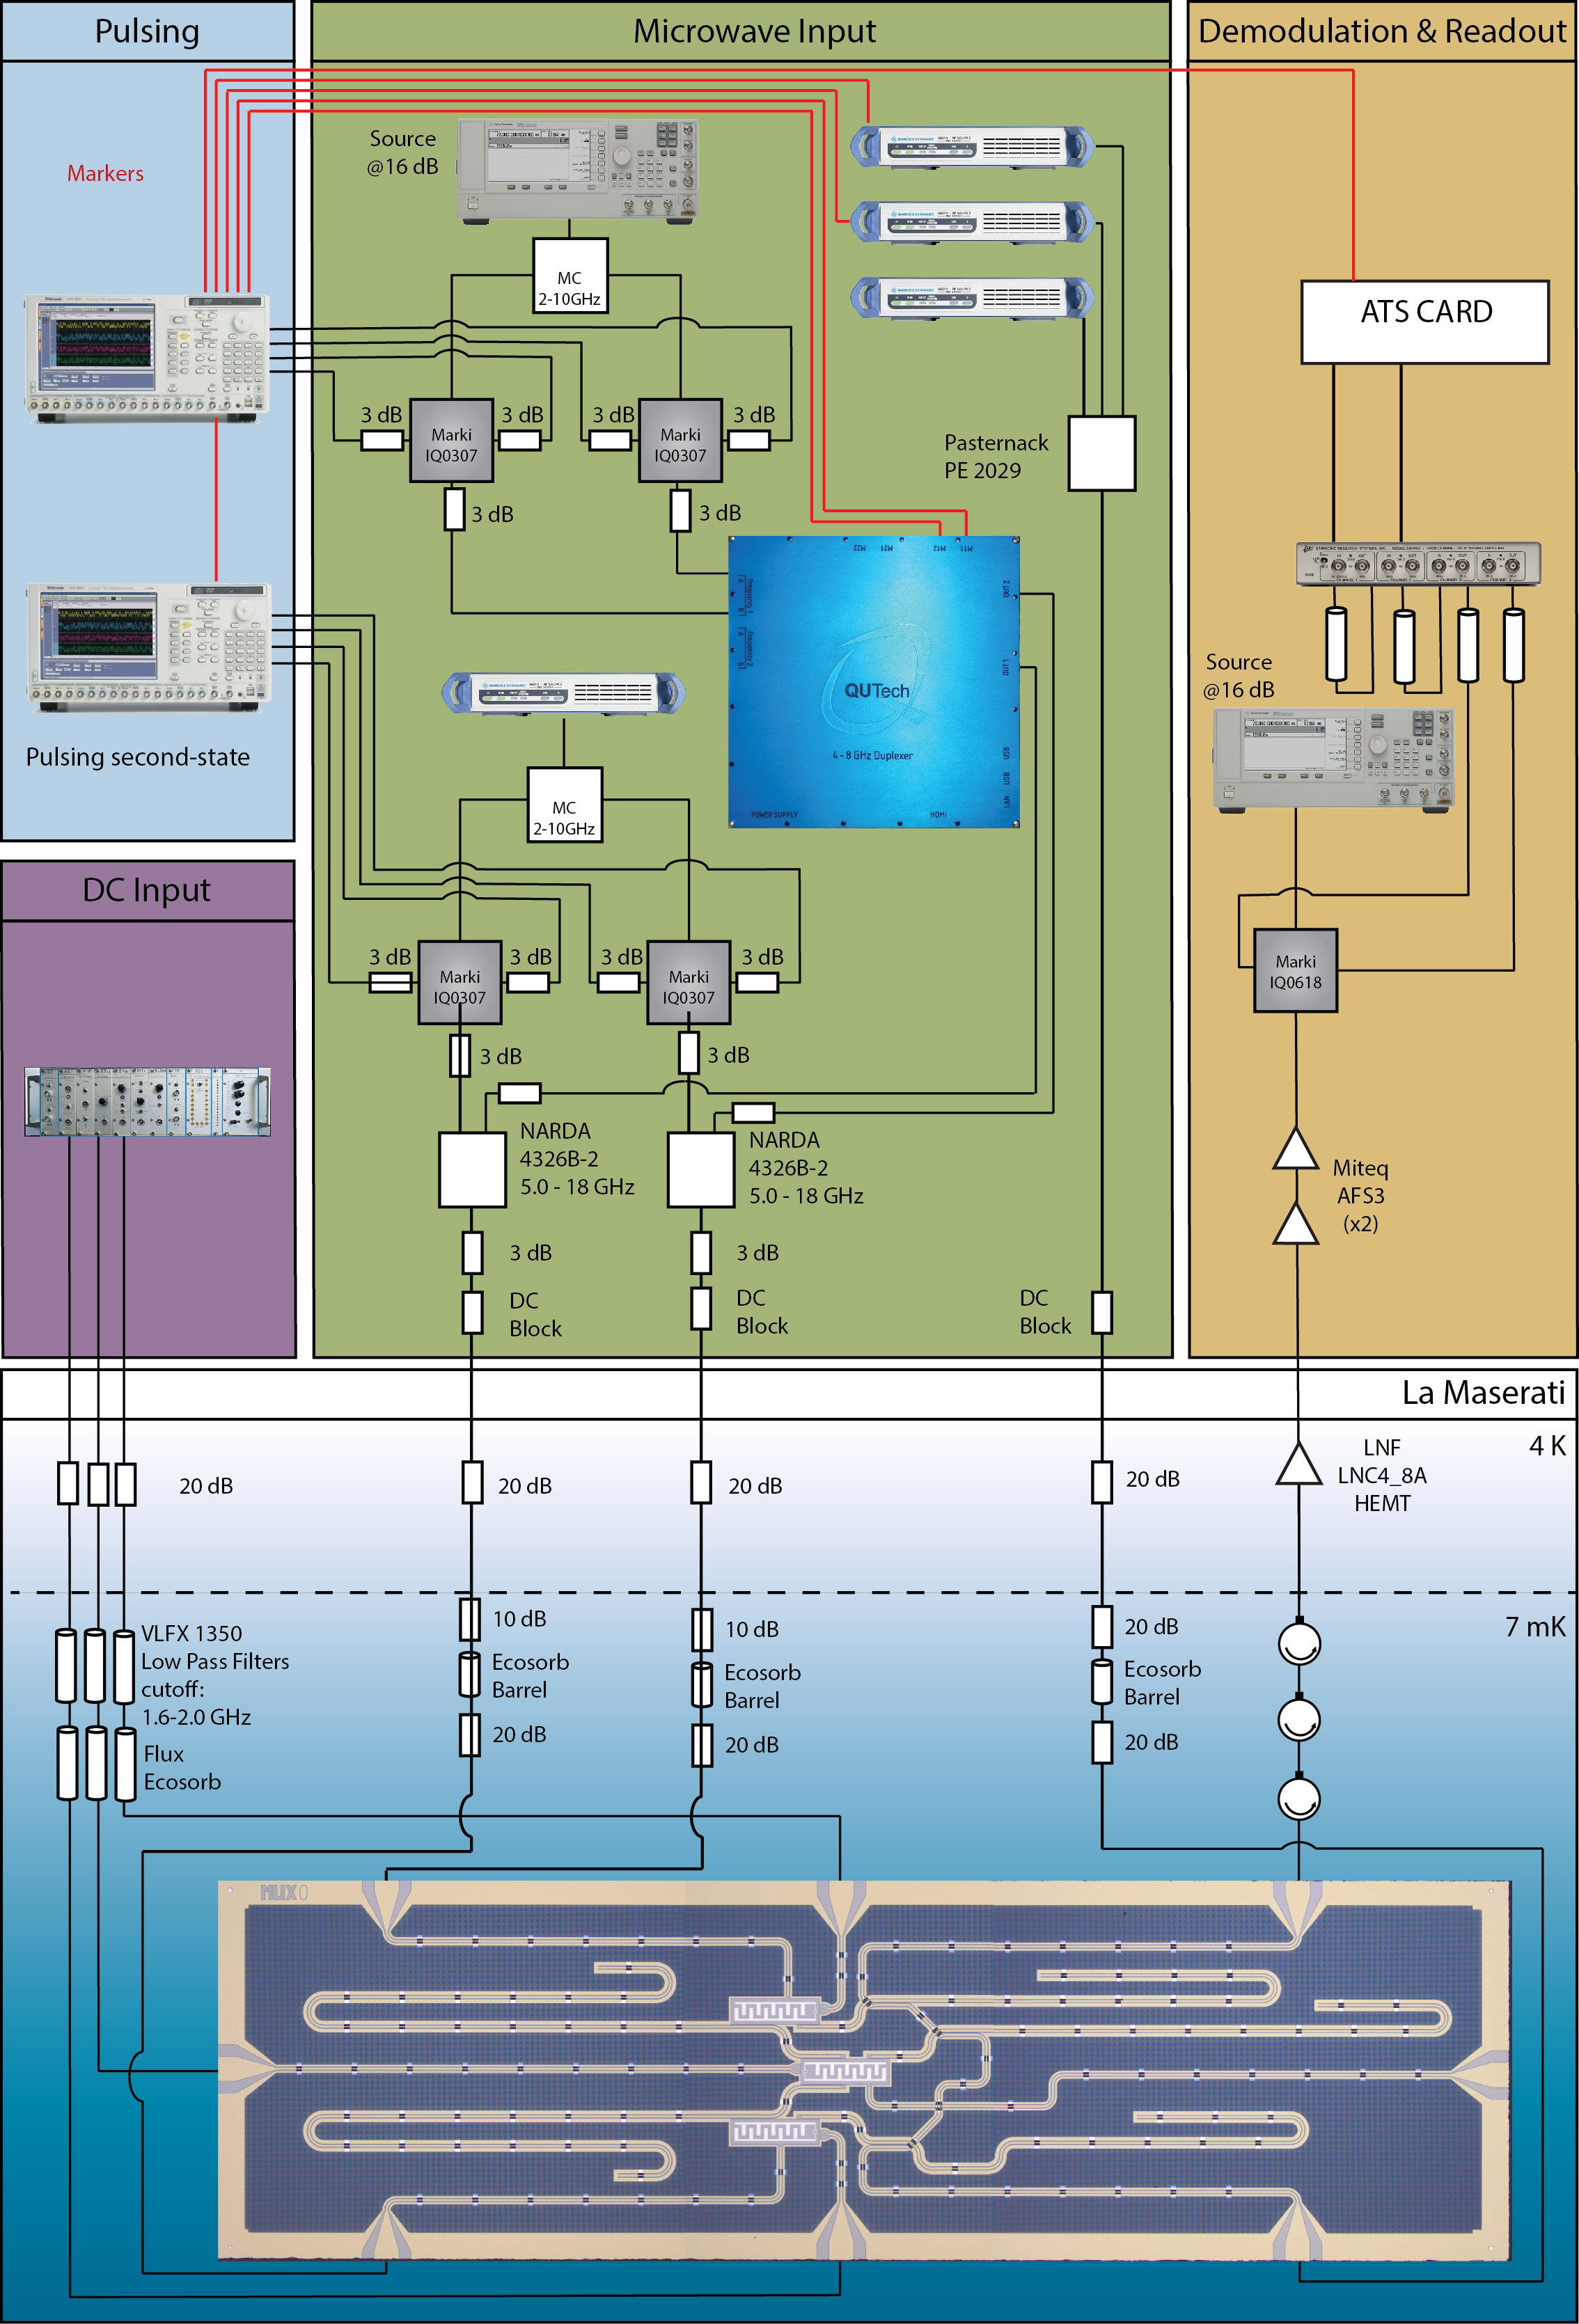
\includegraphics[width=.9\textwidth]{../Figures/20150512_Muxmon_Setup.jpg}
        \caption{The Muxmon set-up}
        \label{fig:Muxmon set-up}
      \end{figure}

      The Muxmon experiment set-up is shown in Figure~\ref{fig:Muxmon set-up}. The main AWG is used for generating the Gaussian and DRAG pulses, and to trigger other devices. A second AWG is used for pulses at the excited-state to second excited-state transition frequency. Two of the four input ports of the Duplexer are used. One input port receives the main pulse, the other receives the DRAG pulse (see Section~\ref{ssec:qubit control} for more info). The main pulse and DRAG pulse are combined in the Duplexer. The output ports are connected to the drive lines of the top and bottom qubit.

  \chapter{Muxmon device characterization}
    \label{ch:Muxmon device characterization}

    This chapter describes the measurements performed to characterize the Muxmon chip. Section~\ref{sec:The transmon} gives a short introduction of the transmon qubit. The initial characterization of the chip is done using continuous-wave measurements, described in Section~\ref{sec:Continuous-wave measurements}. These are measurements used to determine properties such as the energy levels of the resonators and qubits. Once the energy levels of the resonators and qubits are found, the specific properties of the qubits, such as their decoherence times, can be measured. These measurements are known as time-domain measurements, and are described in Section\ref{sec:Time-domain measurements}. With the qubits characterized, in Section~\ref{sec:Exploring Frequency re-use} frequency re-use is studied by tuning the top and bottom qubit to the same frequency.

    \section{The transmon}
      \label{sec:The transmon}
      The qubits on the Muxmon chip are all transmon qubits, which are modified versions of the Cooper-pair box qubit \cite{bouchiat1998CooperPairBox,nakamura1999coherent}. The Cooper-pair box qubit consists of a superconducting island separated from a superconducting bulk by a Josephson junction. The Josephson junction allows Cooper-pairs to travel between the island and the bulk. The Hamiltonian describing the Cooper-pair box is given by:

      \begin{equation}
        H=4 E_C (n - n_g)^2-E_J \cos \phi
        \label{eq:Cooper-pair box Hamiltonian}
      \end{equation}

      Here $E_C$ is charging energy, $E_J$ is the Josephson energy, $n$ is the operator corresponding to the number of Cooper pairs on the island, $n_g$ is a charge offset, and $\phi$ is the Josephson phase operator. The Cooper-pair box operates in the regime where $E_C \gg E_J$, resulting in well-defined number of Cooper pairs on the island, which determine its energy levels. The Cooper-pair box is therefore known as a charge qubit. The Josephson junction is a nonlinear inductor, resulting in an anharmonicity between the energy levels of the Cooper-pair box. Due to tihs anhamonicity the different energy levels can be individually addressed, which is crucial for a qubit. The qubit states in a Cooper-pair box qubit are the two states having the lowest energy $\ket{n}$ and $\ket{n+1}$. The number of Cooper pairs $n$ having the lowest energy is determined by an applied gate voltage, corresponding to $n_g$.

      The Cooper-pair box qubit suffers from being sensitive to fluctuations in the charge offset $n_g$, which result in fluctuations in its energy levels. The transmon qubit is a modification to the Cooper-pair box, which is insensitive to charge fluctuations by operating the regime where $E_J \gg E_C$ \cite{koch2007Transmon,schreier2008suppressing}. This is achieved by adding a large shunting capacitor to the Cooper-pair box, which increases its capacitance to ground, thereby reducing $E_C$. The charge sensitivity decreases exponentially with increasing $E_J/E_C$ ratio. The cost of increasing $E_J/E_C$ is that the anharmonicity between the energy levels decreases, albeit with a polynomial depence. The transmon usually operates in the regime where $E_J/E_C$ is somewhere between $20$ and $100$, where the charge sensitivity is largely suppressed, while still having sufficient anharmonicity. In the transmon regime the transition frequency from the ground-state to the excited-state of the qubit is given to good approximation by \cite[p.52]{Reed}:

      \begin{equation}
        \hbar \omega_q = \sqrt{8 E_J E_C} - E_C
        \label{eq:transmon frequency}
      \end{equation}

      The performance of a qubit is determined by its ability to retain information, which are quantified by its decoherence times. The more isolated a qubit is from its environment, the less decay channels it will have, and the longer its decoherence times will be. On the other hand it is also necessary to interact with the qubit. In a cQED chip a signal is sent through a feedline. Directly connecting a qubit to this feedline would result in a strong decay channel. The connection between a transmon and the feedline is therefore mediated by a capacitive coupling to a resonator, in this case a coplanar waveguide (see Part I). The resonator acts as a filter, thereby limiting the decay channel. Nevertheless due to the Purcell effect the resonator is still a decay channel for the qubit, the rate of which depends on the quality factor of the resonator.

    \section{Continuous-wave measurements}
      \label{sec:Continuous-wave measurements}
      The first step in the characterization of a chip is to look for signs of life, which are the energy levels of the resonators and qubits. These manifest themselves as resonance frequencies of the resonators and of the qubits that are coupled to them. To determine the energy levels we send continuous tones through the feedline, and measure response in the transmission $S_{21}$. These measurements are known as continuous-wave measurements.

      \subsection{Scanning for resonators}
        \label{sec:resonator-scan}
        Since communication with the qubits is mediated through their capacitive coupling to resonators, the first step is to find the resonator frequencies. This is done using a transmission measurement of the feedline, in combination with heterodyne detection, and has been explained in section \textbf{TODO:} Create section in Resonator chapter.

        There is one difference in measuring a resonator when there is a qubit coupled to it. When considering the qubit as a two-level system, the behaviour of the coupled resonator-qubit system is governed by the Jaynes-Cummings Hamiltonian \cite{koch2007Transmon}:

        \begin{equation}
          \hat{H} = \hbar \wres\left(\hat{a}^\dagger \hat{a} + \frac{1}{2} \right) + \frac{\hbar \wqub}{2}\hat{\sigma}_z + \hbar g \left(\hat{a}^\dagger \sigma_{-} + \hat{a}\sigma_{+}\right)
          \label{eq:Jaynes-Cummings}
        \end{equation}

        where $\wres$ is the bare resonance frequency of the resonator, $\wqub$ is the resonance frequency of the qubit's ground-to-excited-state transition, and the qubit's two states are in the spin-representation. This Hamiltonian consists of three terms. The first term corresponds to the energy level of the resonator, the second to the energy level of the transmon, and the third is an interaction term between the two with coupling strength $g$. The coupling strength $g$ determines the rate at which the qubit and resonator exchange excitation. If $g$ is larger than the decay rates of both the resonator and qubit, the system is in the strong-coupling regime, and so an excitation can travel multiple times between the resonator and qubit before decaying.

        The difference between the resonator frequency $\wres$ and the qubit frequency $\wqub$ is given by the detuning $\Delta = \wqub - \wres$. If the magnitude of the detuning is large compared to the coupling strength $g$, the system is in the dispersive regime. In this case the Hamiltonian can be approximated by the dispersive Jaynes-Cummings Hamiltonian:

        \begin{equation}
          \hat{H} = \frac{\hbar \wqub^{'}}{2} \hat{\sigma}_z +  \left(\hbar \wres^{'} + \hbar \chi \hat{\sigma}_z\right) \hat{a}^\dagger \hat{a}
          \label{eq:dispersive-Jaynes-Cummings}
        \end{equation}

        The coupling between the qubit and resonator causes both the qubit frequency and the resonator frequency to shift: $\wqub^{'} = \wqub + \chi_{01}$, $\wres^{'}=\wres - \chi_{12}/2$, where $\chi_{ij} = \frac{g_{ij}^2}{\omega_{ij}-\omega_r}$ are the partial dispersive shifts. We see that in this approximation we must not only take into account the lowest two states of the transmon, but also the second excited-state of the transmon. The difference between the first excited-state to second excited-state transition frequency $\omega_{12}$ and the ground-state to first excited-state transition frequency $\omega_{01}$ is given by the anharmonicity $\alpha=\omega_{12} - \omega_{01} \simeq E_C$ \cite{koch2007Transmon}. The anharmonicity $\alpha$ determines the degree in which the transmon behaves as a qubit, without experiences excitations to higher excited-states.

        Aside from experiencing a frequency shift dependent on the amount of detuning, Equation~\ref{eq:dispersive-Jaynes-Cummings} shows that the resonator also experiences a shift depending on the state of the qubit. The resonator's frequency is decreased by an amount $2 \chi$ when the qubit is in the excited-state. The parameter $\chi$ is the dispersive shift, and is given by:

        \begin{equation}
          \chi = \chi_{01} - \chi_{12}/2 \approx \frac{g^2}{\Delta}\frac{\Ec}{\hbar \Delta - \Ec}
          \label{eq:dispersive-shift}
        \end{equation}

        Due to this coupling between resonator and qubit, it is important to choose the right RF power. When the amount of photons in the resonator reaches a critical photon number, this coupling will result in the resonator experiencing nonlinear effects. The resonator will thereby lose its Lorentzian lineshape. Therefore the RF power should be kept sufficiently low to avoid these nonlinear effects, while still maintaining a good signal-to-noise ratio.

        \begin{figure}[tb]
          \centering
          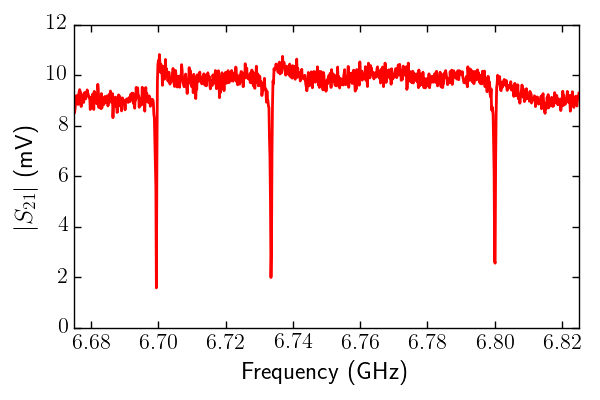
\includegraphics[width=.7\textwidth]{../Figures/Qubit characterization/Resonator scans.png}
          \caption{The three resonators coupled to the top, ancilla, and bottom qubits in ascending frequency.}
          \label{fig:Three resonators}
        \end{figure}

        In Figure~\ref{fig:Three resonators} the three resonators belonging to the top, ancilla, and bottom qubit are shown, with resonator frequencies \SI{6.700}{\giga \hertz}, \SI{6.733}{\giga \hertz}, and \SI{6.800}{\giga \hertz} respectively.

      \subsection{Powersweeping the resonators}
        \label{ssec:powersweep}

        \begin{wrapfigure}[15]{r}{0.55\textwidth}
          \begin{center}
          \vspace{-30pt}
            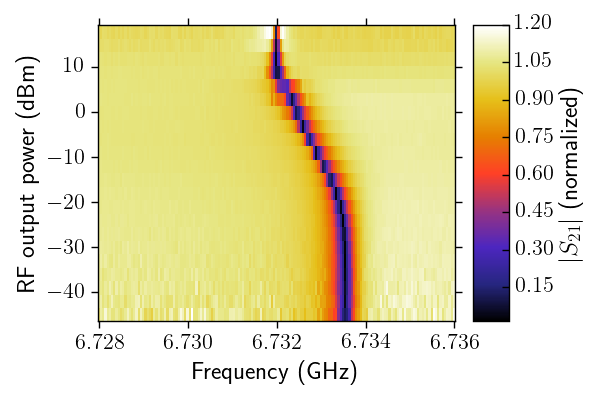
\includegraphics[width=\textwidth]{../Figures/Qubit characterization/Powersweep.png}
          \end{center}
          \vspace{-20 pt}
          \caption{A powersweep of the resonator coupled to the ancilla qubit. The dispersive shift found is equal to $\chi\approx$\SI{30}{\mega \hertz}.}
          \label{fig:powersweep}
        \end{wrapfigure}

        Once the resonators have been located, the next stage is to find the qubit that is capacitively coupled to each of the resonators. First some initial measurements are performed aimed at gaining information about our resonator and qubit, which will allow us to search for the qubit frequencies with more focus.

        As explained previously, the capacitive coupling between the resonator and qubit shifts the resonator frequency $\wres$ from its bare frequency. When the amount of photons in the resonator reaches a certain point, the resonator experiences nonlinearity, thereby losing its Lorentzian lineshape. When increasing the RF power even further, at a certain point the resonator regains its Lorentzian lineshape. In doing so its resonance frequency has shifted to its bare frequency $\wbare$. For more information see Reed's thesis~\cite{Reed}. Observing this frequency shift reveals that a qubit is coupled to the resonator. This frequency shift is commonly measured in a powersweep, where a resonator scan is performed for a range of powers. In Figure~\ref{fig:powersweep} a powersweep is shown of the ancilla qubit. As can be seen the resonator frequency shifts during the transition from the low-power regime to the high-power regime. Since the resonator frequency shifts downwards when entering the high-power regime it can be concluded that the ancilla qubit frequency lies below the resonator frequency.

        A powersweep additionally provides information about at what power the resonator enters the nonlinear regime. For measurements involving the qubit the readout power must be below this threshold power. Furthermore, from the frequency shift between the dressed cavity frequency and the bare cavity frequency, the amount of detuning between the qubit and the resonator can be estimated using Equation~\ref{eq:dispersive-shift}.

        If no shift is observed, it could mean that the qubit is dead, due to an open or shorted Josephson junction. However, this is not necessarily the case. An alternative possibility is that the detuning between qubit and resonator is very large, and as a result the frequency shift cannot be discerned.

      \subsection{Scan for qubit sweet-spots}
        \label{Scan for qubit sweet-spots}
        All qubits in the Muxmon device have a tunable resonance frequency. This is achieved by replacing the Josephson junction with a superconducting quantum interference device (SQUID). In this case the two islands that compose the transmon qubit are connected by two Josephson junctions instead of one, effectively forming a loop. If the two Josephson junctions in a SQUID loop have the same Josephson energy $E_J=E_{J1}=E_{J2}$, this results in an effective Josephson energy~\cite[pp.54-56]{Reed}:

        \begin{equation}
          E_J^\text{eff}=2E_J*\cos{\left( \pi \frac{\Phi}{\Phi_0} \right)}
          \label{eq:Josephson energy}
        \end{equation}

        where $\Phi_0=h/2e$ is the magnetic flux quantum and $\Phi$ is the flux passing through the SQUID loop.

        As can be seen in Equation~\ref{eq:Josephson energy}, the effective Josephson energy $E_J^\text{eff}$ of a SQUID loop can be controlled by the flux through the SQUID loop. This is commonly done by having a flux bias line in close proximity to the SQUID loop. Current flowing through the flux-bias line alters the magnetic field in the vicinity of the SQUID loop, thereby changing the amount of flux through the SQUID loop. A fixed current from a digital-to-analog (DAC) converter is used to set the flux through the SQUID loop, thereby changing the effective Josephson energy $E_J^\text{eff}$. According to Equation~\ref{eq:transmon frequency} the qubit frequency depends on the Josephson energy, and so changing the magnetic flux through the SQUID loop changes the qubit frequency. Qubits having a SQUID loop are therefore called flux-tunable. Since the effective Josephson energy $E_J^\text{eff}$ has a cosine-dependence on the flux, the qubit frequency is periodic with respect to the flux. It- has a maximum when $\Phi$ is a multiple of $\Phi_0$, in which case the qubit is said to be at its sweet-spot.

        \begin{wrapfigure}[14]{r}{0.45\textwidth}
          \begin{center}
          \vspace{-30pt}
            \includegraphics[width=\textwidth]{../Figures/Muxmon SQUID loop w annotation.png}
          \end{center}
          \vspace{-20 pt}
          \caption{A SQUID loop (1) in close proximity to a flux-bias line (2).}
          \label{fig:SQUID loop}
        \end{wrapfigure}
        For flux-tunable qubits, flux corresponding to the sweet-spot of the qubit can be found without knowledge of the qubit frequency. This can be done by sweeping the DAC current and measuring the shift in the resonator frequency. Because the qubit frequency varies as the current through the flux-bias line changes, the detuning between the qubit and the resonator changes. As a result the dispersive shift $\chi$, and therefore the resonator frequency, also varies. At the sweet-spot of the qubit, the resonator's frequency $\wres$ is at a maximum. This is irrespective of whether the qubit's frequency $\wqub$ is above or below the resonator's frequency.

        Finding the sweet-spot can be done by performing a series of resonator scans as the DAC voltage is varied. The result of such a 2D scan shown in Figure~\ref{fig:tracked spectroscopy}. There is an alternative, faster measurement which can be performed, and is explained in Appendix~\ref{Finding the qubit sweet-spot using a one-dimensional scan}. It is not necessarily the case that the qubit sweet-spot is at zero DAC current, as trapped magnetic flux may result in a flux offset.

        In the case where the powersweep showed no measurable frequency shift, these measurements are also useful in discerning whether or not the qubit actually has broken junctions, or whether it was simply far detuned from the resonator.

      \subsection{Qubit spectroscopy}
        \label{sec:spectroscopy}

        The measurement to perform in order to find the qubit depends on the amount of detuning between the resonator and qubit, which can be estimated from powersweep measurements. If the amount of detuning is large compared to the coupling strength ($\Delta \gg  g$), the system is in the dispersive regime. In this case one commonly performs a two-tone spectroscopy to find the qubit's frequency. If the detuning is comparable to the coupling strength ($\Delta \sim g$), the qubit and resonator are hybridized, and experience an avoided crossing. In such cases a normal transmission measurement suffices. In the Muxmon device the sweet-spot frequencies of all qubits were considerably lower than their corresponding resonator frequencies, and so the qubits were always in the dispersive regime. Therefore two-tone spectroscopy was performed to find the qubit frequencies.

        When finding the qubits the DAC currents were chosen such that the qubits were close to their sweet-spots. It is important that the qubit is not close to its anti-sweet-spot, which would make it difficult, if not impossible to find.

        \begin{figure}[tb]
          \centering
          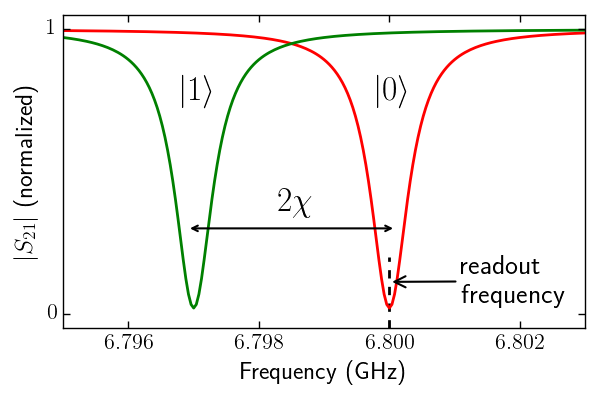
\includegraphics[width=.5\textwidth]{../Figures/Qubit characterization/dispersive shift.png}
          \caption{The resonator frequency shifts by an amount $2\chi$ dependent on the state of the qubit, where $\chi$ is the dispersive shift. In a two-tone spectroscopy measurement the readout frequency is fixed at the resonant frequency of the top qubit, while a second tone is swept with varying frequency. The transmission is low when the second tone is off-resonant with the qubit frequency and high if the second tone is resonant with the qubit frequency.}
          \label{fig:dispersive shift}
        \end{figure}

        As was explained in section~\ref{sec:resonator-scan}, in the dispersive regime the resonator experiences a $2 \chi$ frequency shift dependent on the state of the qubit. This is shown in Figure~\ref{fig:dispersive shift}. For a resonator capacitively coupled to the feedline, the transmission experiences a dip at the resonator frequency, which shifts when the qubit's state is switched. The transmission at the resonator's dip when the qubit is in the ground state will therefore be dependent on the state of the qubit (low when the qubit is in the ground state, high when the qubit is in the excited-state). This is the property exploited in a two-tone spectroscopy measurement.

        In a two-tone spectroscopy measurement two tones are sent through the feedline.
        \begin{enumerate}
          \item A drive tone with varying frequency $\wdrive$.
          \item A readout tone at the resonator frequency when the qubit is in the ground state.
        \end{enumerate}

        \begin{wrapfigure}[20]{r}{0.45\textwidth}
          \begin{center}
          \vspace{-30pt}
            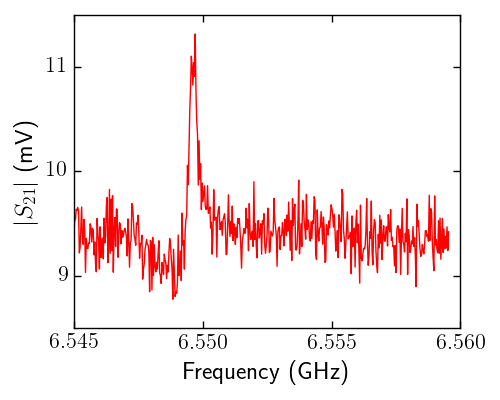
\includegraphics[width=\textwidth]{../Figures/Qubit characterization/Spectroscopy.png}
          \end{center}
          \vspace{-20 pt}
          \caption{Two-tone spectroscopy performed on the ancilla qubit at its sweet-spot. The transmission is low when the drive tone is off-resonant with the qubit frequency. However, when the drive tone approaches the qubit frequency, the resonator frequency experiences a dispersive shift, resulting in enhanced transmission.}
          \label{fig:qubit spectroscopy}
        \end{wrapfigure}

        In figure~\ref{fig:qubit spectroscopy} the result of a two-tone spectroscopy is shown. When the drive frequency $\wdrive$ is detuned from the qubit's frequency $\wqub$, the drive is off-resonant with respect to the qubit, and so we measure a low transmission due to the readout tone being at the resonator frequency. However, when the drive frequency $\wdrive$ approaches the qubit's frequency $\wqub$ the qubit will start to oscillate between its ground- and excited-state, at a rate dependent on the detuning between the drive frequency $\wdrive$ and the qubit's frequency $\wqub$. The qubit will therefore have a partial population in the excited-state, resulting in a shift of the resonator frequency, dependent on the population in the excited-state. The result is an increase in transmission

        The minimum linewidth of the qubit using spectroscopy is set by its dephasing time $T_2$, which can be seen as the uncertainty in its frequency. However, the power of the drive tone causes an additional increase in the linewidth, due to stimulated emission of the qubit. This effect is known as power broadening, and can be quite useful for finding qubits, especially when designing high-quality qubits with a very narrow intrinsic linewidth. The optimal power for the drive strength is further dependent on the amount of detuning $\Delta$ between the qubit and resonator. The resonator effectively acts as a bandpass filter, centered around the resonator frequency. Therefore, the stronger the detuning, the more the drive tone is suppressed.


        The dispersive shift $2 \chi$ is also dependent on the amount of detuning $\Delta$ between the qubit and resonator. If the detuning $\Delta$ is large, the dispersive shift will be very small, and so the difference in transmission will also decrease. Since the resonator has a Lorentzian lineshape, at the resonance frequency this Lorentzian is flat, and so is insensitive to small deviations. To increase the contrast between the resonant and off-resonant transmission, it is usually advantageous to measure at a slight detuning $\delta$ away from the resonance frequency, where the transmission slope is high. Since the resonator frequency shifts down when the qubit is excited, it is better to have a positive detuning $\delta$ to ensure that the transmission increases as the drive frequence $\wdrive$ approaches the qubit frequency $\wqub$ and decreases as it leaves the qubit frequency.

        A better approach to a two-tone spectroscopy measurement is to separate the drive tone and the readout tone in time. This is known as pulsed spectroscopy, and has the advantage that during readout the photon population in the resonator will be low, resulting in a more accurate measurement. This does, however, require a more complicated set-up, where the pulses need to be accurately timed.

        % \subsubsection{Avoided crossing}
        %   When the detuning $\Delta$ between the qubit and resonator is not large compared to their coupling strength $g$, the qubit and resonator experience an avoided crossing. Because all of the qubits in the Muxmon chips are considerably lower in frequency compared to their resonators, the system is always in the dispersive regime, and so the system never approaches the avoided crossing. Nevertheless it is worth mentioning the avoided crossing briefly, as it is a breeding ground for interesting physics.

        %   At the avoided crossing the system is not in the dispersive regime, and so the dispersive Jaynes-Cummings Hamiltonian no longer applies. In this case the resonator and qubit are hybridized, and one can no longer speak of a qubit and resonator as separate entities. Instead, this hybridization results in a so-called quton and phobit.

        %   \textbf{Avoided crossing info:}
        %   \begin{itemize}
        %     \item The coupling strength $g$ is the minimum distance be~tween the splitting
        %     \item From Reed's thesis p.63 explanation of this avoided crossing is given\\
        %     \begin{align}
        %      E_0 = & -\frac{\hbar \Delta}{2}\\
        %      E_1 = & n \hbar\omega_r \pm \frac{\hbar}{2}\sqrt{4g^2n + \Delta^2}
        %     \end{align}\\
        %     Joining $E_0 + E_1$ results in a qubit approaching a resonator from the top.\\
        %     When the frequency of the qubit equals that of the resonator, the energy difference reaches a minimum, and is equal to $2g$.
        %   \end{itemize}

        %   \textbf{TODO:} Avoided crossing
        %   \begin{itemize}
        %     \item Explain the quton fobit behaviour near the avoided crossing
        %     \item Explain how one can extract coupling from avoided crossing
        %     \item Explain that for the Muxmon qubit this effect is not present
        %     \item Explain multiple lines near avoided crossing
        %   \end{itemize}

        %   \textbf{figures:}
        %   \begin{itemize}
        %     \item Figure of avoided crossing
        %   \end{itemize}


      \subsection{Tracking the qubits}
        \label{ssec:tracked spectroscopy}

        \begin{wrapfigure}[20]{r}{0.45\textwidth}
          \begin{center}
          \vspace{-30pt}
            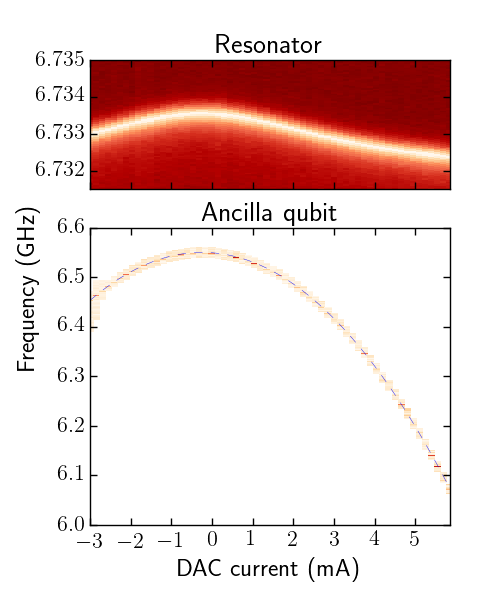
\includegraphics[width=\textwidth]{../Figures/Qubit characterization/Tracked_spectroscopy.png}
          \end{center}
          \vspace{-20 pt}
          \caption{Tracked spectroscopy of the ancilla qubit. The blue dotted line is the corresponding fit to the qubit frequency, showing excellent agreement with measurements.}
          \label{fig:tracked spectroscopy}
        \end{wrapfigure}

        For flux-tunable qubits one is usually not interested in finding the frequency at one specific flux value, but how this frequency changes with varying flux. A simple approach is to perform a two-dimensional scan of a fixed frequency range versus flux. This however has several disadvantages. First of all it requires a new measurement to be set-up every time the qubit frequency moves out of the frequency range. Furthermore the largest part of the measurement will be spent measuring off-resonant signal, containing no useful information.

        As an alternative approach I have created a modified version of the spectroscopy versus flux scan, known as tracked spectroscopy. In this approach after every spectroscopy scan the qubit frequency is extracted through fitting. From the qubit frequencies measured in previous scans the expected frequency at the next flux value is extrapolated. The frequency window of the next spectroscopy scan are then centered around the expected qubit frequency. The qubit is therefore tracked as its frequency changes, without requiring any human intervention. The same method is applied to update the resonator frequency. For more information on the tracked spectroscopy algorithm see appendix~\ref{sec:Tracked spectroscopy}.

        In Figure~\ref{fig:tracked spectroscopy} the results of tracked spectroscopy are shown for the ancilla frequency. As can be seen the qubit is tracked over a wide range of frequencies, while the frequency window in each scan is relatively small. As the qubit frequency approaches the resonator frequency, the dispersive shift $\chi$ increases, and so the resonator frequency shifts upwards. InIn this scan one can clearly see the sweet-spot of the qubit, and the curve has the shape of the square root of a cosine, consistent with Equations~\ref{eq:transmon frequency} and~\ref{eq:Josephson energy}.

      \subsection{Second transition of the qubit}
        \label{ssec:12-transition spectroscopy}
        Once the qubit's grequency is known, it is possible to find the qubit's excited-state to second-excited-state transition $\omega_q^{12}$, which shall be referred to as the 12-transition. For consistent notation we shall temporarily denote the qubit's ground-state to excited-state transition frequency as $\omega_q^{01}$. The anharmonicity $\alpha$ is then given by the difference in transition frequencies: $\alpha = \omega_q^{12} - \omega_q^{01}$. Knowledge of the anharmonicity $\alpha$ allows determination of the coupling energy $E_c$ through \textbf{TODO:}.

        The 12-transition can be found using three-tone spectroscopy, in a manner similar to two-tone spectropscopy measurement explained in section~\ref{sec:spectroscopy}. The following three tones are used in three-tone-spectroscopy:

        \begin{enumerate}
          \item A drive tone with fixed frequency $\omega_\text{drive}^{01}$ at the qubit frequency $\omega_q^{01}$.
          \item A drive tone with varying frequency $\omega_\text{drive}^{12}$ to scan for the 12-transition.
          \item A third tone at the resonator frequency when the qubit is in the excited-state.
        \end{enumerate}

        The first drive tone with frequency $\omega_\text{drive}^{01}$ is used the drive the qubit to the excited-state. Since the first drive tone results in the excited-state being (partially) populated, the second tone with frequency $\omega_\text{drive}^{12}$ is then able to drive the qubit from the excited-state to the second-excited-state. The transmission should therefore change when $\omega_\text{drive}^{12}$ is on resonance with $\omega_q^{12}$.

        \begin{figure}[tb]
          \centering
          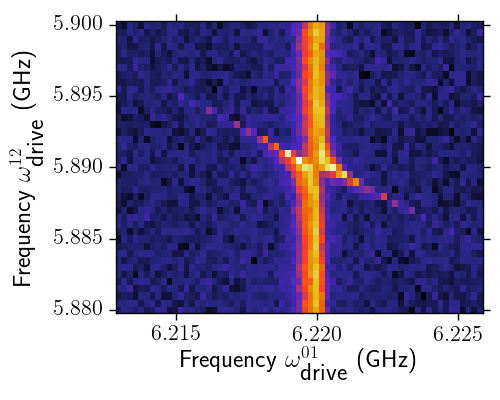
\includegraphics[width=.6\textwidth]{../Figures/Qubit characterization/second transition spec.png}
          \caption{Two-dimensional three-tone pulsed spectroscopy results for the bottom qubit while at its sweet-spot. The second-excited state has a frequency equal to $\omega_{12}=\SIm{5.89}{\giga \hertz}$, corresponding to an anharmonicity $\alpha= \omega_{12}-\omega_{01}=\SIm{-330}{\mega \hertz}$.}
          \label{fig:Second excited state spectroscopy}
        \end{figure}

        In principle the first drive tone with frequency $\omega_\text{drive}^{01}$ can be kept fixed at the 01-transition frequency $\omega_q^{01}$. However, by performing a two-dimensional scan, where $\omega_\text{drive}^{01}$ is also varied in a small region around $\omega_q^{01}$, the 12-transition becomes much clearer. This can be seen in Figure~\ref{fig:Second excited state spectroscopy}, where a shift in transmission is observed when $\omega_\text{drive}^{01} = \omega_q^{01}$. This corresponds to the 12-transmission frequency $\omega_q^{12}$. Additionally, a transmission shift is observed at a line crossing $\omega_q^{12}$. At this line $\omega_q^{01} + \omega_q^{12} = \omega_q^{02}$, resulting in some population in the second-excited-state.


        It is worthwhile to note that three-tone spectroscopy produces much more accurate results when using pulsed spectroscopy, as the difference in transmission is generally small compared to two-tone spectroscopy.

        Finding the resonator frequency when the qubit is in the excited-state can be tricky, as pulsed spectroscopy is usually required. Nevertheless a rough estimation can be found using a modified version of spectroscopy, where the drive tone $\omega_\text{drive}$ is kept fixed, while the resonator frequency is swept. The lower peak will be a rough estimation of the resonator frequency when the qubit is in the excited-state. Alternatively it is also possible to use the resonator frequency when the qubit is in the ground-state, although this will reduce the contrast between driving on-resonance and driving off-resonance.

        \begin{itemize}
           \item Once the 12-transition transition is found, and hence the qubit's anharmonicity $\alpha$, it is the possible to calculate the coupling energy $E_c$. \textbf{TODO:} cite Reed.
        \end{itemize}

      \subsection{Flux matrix}
        \label{ssec:Flux matrix}

        \begin{figure}[tb]
          \centering
          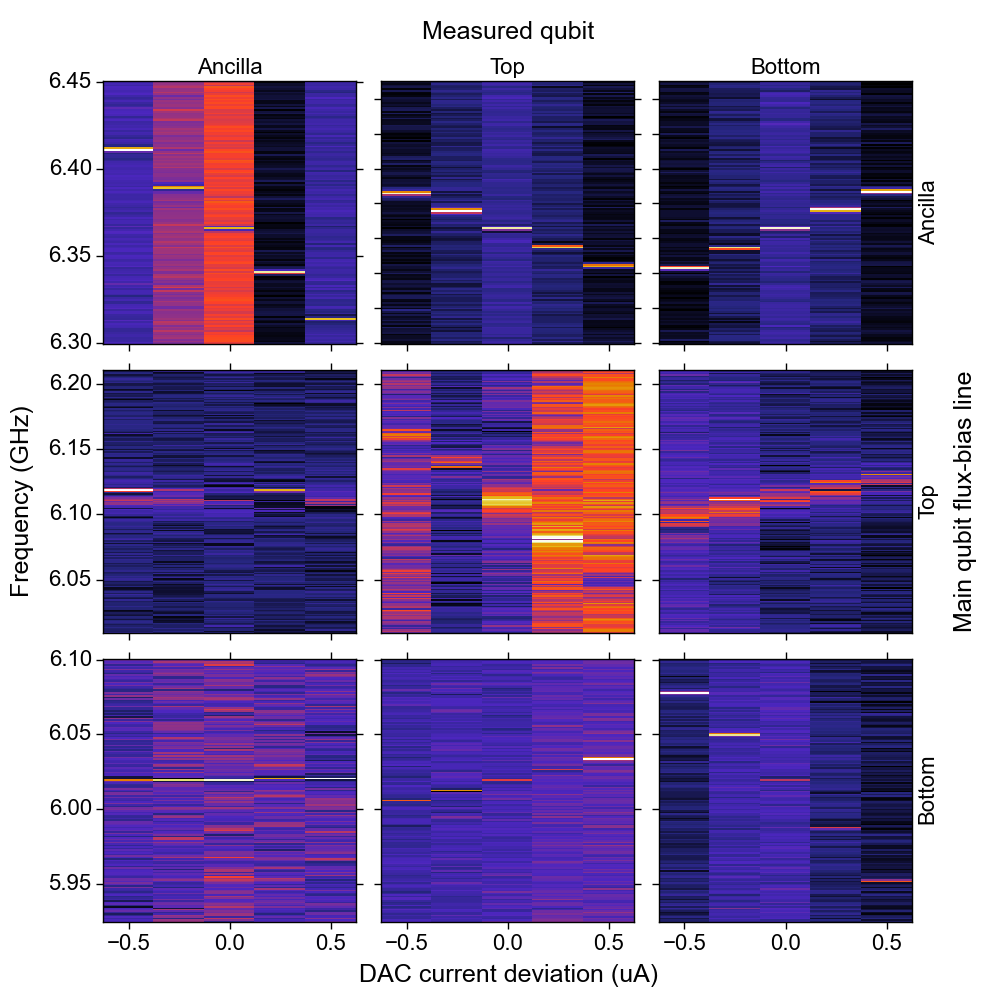
\includegraphics[width=\textwidth]{../Figures/Qubit characterization/Flux_matrix.png}
          \caption{Frequency responses of each qubit to each flux-bias line. Each qubit has been tuned away from its sweet-spot such that the frequency-response is higher. The frequency response slopes determine the coefficients of matrix $\boldsymbol{M}$, used for creating the flux matrix $\boldsymbol{F}$.}
          \label{fig:flux matrix}
        \end{figure}
        When a current is passed through a flux-bias line, it is not only the flux through the SQUID of the qubit directly connected to it that is affected. Instead, the fluxes through SQUIDs of neighbouring qubits are also affected, albeit to a lesser extent. Therefore changing the frequency of one qubit by changing its corresponding flux-bias line current also affects the frequencies of the other flux-tunable qubits on the chip. For the Muxmon experiment the frequencies of the three qubits have to be individually tuned to very specific frequencies, and so the frequency responses of the qubits have to be decoupled. This is done by implementing a flux matrix, which corrects for the flux cross-coupling effects.

        A flux matrix $\boldsymbol{F}$ is an $n \times n$ matrix, where $n$ is the number of flux-tunable qubits. Each row $F_i = \left[F_{i1}, \dots, F_{in}\right]$ corresponds to the ratio's by which each of the DAC currents should be changed such that only the frequency of qubit $i$ changes while the other frequencies remain fixed. This results in $n$ decoupled virtual flux parameters.

        For a flux matrix $F$ knowledge of the frequency responses of each of the qubits due to each of the flux-bias lines is required. It is important that the qubits are tuned away from their sweet-spots, to a point where the frequency is sensitive to changes in flux. In Figure~\ref{fig:flux matrix} the frequency responses of the three Muxmon qubits to currents flowing through each of the flux-bias lines are shown. As can be seen the degree to which a flux-bias line affects other qubits can be quite severe. From the frequency responses a frequency response matrix $\boldsymbol{M}$ can be constructed:

        \begin{equation}
          \boldsymbol{M} =
          \begin{bmatrix}
            \frac{\partial f_1}{\partial I_1} & \dots & \frac{\partial f_1}{\partial I_n} \\
            \vdots & \ddots & \vdots \\
            \frac{\partial f_n}{\partial I_1} & \dots & \frac{\partial f_n}{\partial I_n}
          \end{bmatrix}
        \end{equation}

        where $\frac{\partial f_i}{\partial I_j}$ is the frequency response of qubit $i$ to a change in the DAC current corresponding to flux-bias line $j$. Each rows $M_i$ should be divided by the frequency response of the main qubit $\frac{\partial f_i}{\partial I_i}$, such that the elements are relative frequency responses. The diagonal elements of matrix $\boldsymbol{M}$ should be equal to one.

        For each qubit $i$ the DAC current $I^0_i$ corresponding to its sweet-spot is known from tracked spectroscopy. However, since the other DAC currents must be set to zero, the corresponding qubits will likely not be at their sweet-spots. There is a certain combination of DAC currents $\vec{I}^{ss}$ where all qubits are at their simultaneous sweet-spot. This can be found using matrix $\boldsymbol{M}$. Since $\boldsymbol{M}$ contains the frequency responses of each qubit to each of the flux-bias lines, the qubit $i$ remains at its sweet-spot as long as $\boldsymbol{M}_i \vec{I}=I^0_i$ holds, where $\vec{I}$ is the vector containing the DAC currents. Therefore the simultaneous sweet-spot $\vec{I}^{ss}$ is found by solving $\boldsymbol{M} \vec{I}^{ss} = \vec{I^0}$, where $\vec{I}^0$ contains the DAC currents of the individual sweet-spots of the qubits.

        The flux matrix $\boldsymbol{F}$ can be found by inverting matrix $\boldsymbol{M}$. As mentioned earlier, each row $F_i$ of matrix $\boldsymbol{F}$ corresponds to the ratio by which the DAC currents of the flux-bias lines need to be varied, such that only the frequency of qubit $i$ is changed. Each row may therefore be multiplied by a different factor, as long as the ratio between the elements in each row remains constant. By dividing each row $F_i$ by $F_{ii}$ the DAC current of the main flux-bias line is equal to its corresponding virtual flux. The main qubit therefore behaves identically when changing the virtual flux, except that all the other qubit frequencies remain fixed.

        A virtual flux vector $\vec{\Phi}=\left[ \phi_1, \dots \phi_n \right]$ can be converted to the corresponding DAC current vector $\vec{I}$ through:

        \begin{equation}
          \vec{I} = \boldsymbol{F} \vec{\Phi} + \vec{I}^{ss}
        \end{equation}

        By adding the simultaneous sweet-spot DAC voltages $\vec{V}^{ss}$, we obtain the additional property that the simultaneous sweet-spot of the virtual fluxes is set to zero.

    \section{Time-domain measurements}
      \label{sec:Time-domain measurements}
      \subsection{Qubit control}
        \label{ssec:qubit control}
        The measurements described so far are able to determine the energy levels of the qubits and resonators using continuous tones. However, for qubit properties such as their decoherence times, time-domain measurements are required. Here well-calibrated pulses accurately control the state of the qubit, and correspond to gates being applied to the qubit.

        A simple time-domain measurement usually consists of two parts: qubit control, and qubit readout. During qubit control precisely timed pulses modify the state of the qubit. During qubit readout a readout tone is applied in a manner similar to spectroscopy. The state of the qubit can be inferred from the response in transmission. More complicated measurements involve feedback, where additional qubit control can be applied depending on the measurement outcome. Feedback measurements are not performed in this experiment, and are therefore beyond the scope of this thesis.

        Measuring the qubit will project its state onto the Z-axis, and so it will be either measured in state $\ket{0}$ or in state $\ket{1}$, with a probability determined by its population in the two states. One single measurement, however, provides little information about the actual populations in the two states before the measurement. To determine the actual population in the two states it is required to repeat the measurement many times. The number of times the qubit is measured in either states is then an estimate for the actual state populations of the qubit.

        \begin{wrapfigure}[14]{r}{0.4\textwidth}
          \begin{center}
          \vspace{-30pt}
            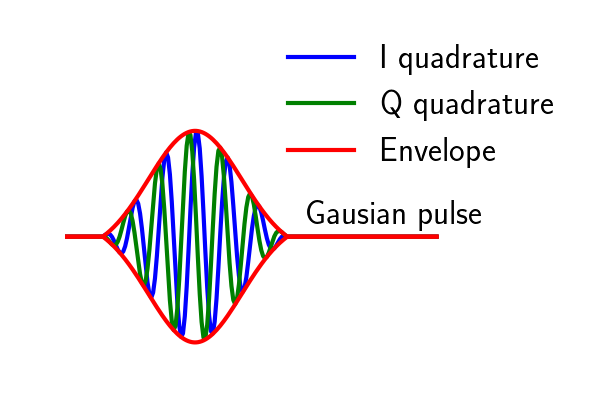
\includegraphics[width=\textwidth]{../Figures/Exploring frequency re-use/Gaussian pulse.png}
          \end{center}
          \vspace{-20 pt}
          \caption{Schematic representation of the Gaussian pulse. The signal is convoluted with a sine and cosine with sideband modulation frequency $\omega_{sb}$, resulting in single-sideband modulation.}
          \label{fig:gaussian pulse}
        \end{wrapfigure}

        Qubit pulses usually have a Gaussian shape, because the corresponding frequency bandwidth is narrow. These pulses can be generated by modulating a carrier signal from an RF generator, and is commonly done using an Arbitrary Waveform Generator (AWG). For the Muxmon experiment the Tektronix AWG5014 is used, which has four voltage channels, each of which can control its voltage output at the nanosecond scale. It further has eight marker channels, which are used to trigger devices, such as RF generators and the Duplexer.

        The carrier signal is sent through the LO port of the mixer, where it is modulated by the AWG. In the Muxmon experiment IQ-modulation is used, and so two AWG channels are used to independently modulate the in-phase and quadrature components of the signal in an IQ-mixer. This allows for single sideband modulation, which shifts the frequency of the signal. Single sideband modulation has the advantage that the carrier frequency $\omega_c$ is shifted away from mixer leakage. For more information on mixer leakage, see section~\ref{sec:Mixer calibration}. A schematic representation of a Gaussian pulse with single sideband modulation is shown in Figure~\ref{fig:gaussian pulse}.

        An important consideration is the duration of a pulse, also known as the pulse length. Shorter pulses allow for more qubit operations within its decoherence time. However, the pulse length is inversely proportional to its frequency bandwidth. If the frequency bandwidth is too broad, there will be a nonnegligible signal at the qubit's excited-state to second excited-state transtion frequency. This will cause leakage to the second excited-state, thereby leaving the two-state Hilbert space. It is therefore desirable to have a bandwidth, which is the inverse of the width $\sigma$ of the Gaussian pulse, that is small compared to the anharmonicity of the qubit.

        Performing gates on qubits requires knowledge of the parameters that define the pulse, such as the amplitude, phase, and pulse duration. The phase determines the axis along which the qubit is rotated. The duration and amplitude of the pulse determine the rotation angle. Rotating the qubit by a specific angle can be achieved by either varying the pulse duration or the pulse amplitude. Both methods have advantages and disadvantages. Varying the pulse duration ensures that the maximum amplitude is roughly fixed, regardless of the rotation angle. Varying the amplitude, on the other hand, ensures that pulses applied to multiple qubits end simultaneously, and so it is more natural to speak of a pulse clock cycle. In the measurements for this thesis the amplitude is varied, while the pulse duration is kept fixed.

      \subsection{Drive amplitude calibration}
        \label{ssec:Rabi}

        \begin{wrapfigure}[15]{r}{0.4\textwidth}
          \begin{center}
          \vspace{-30pt}
            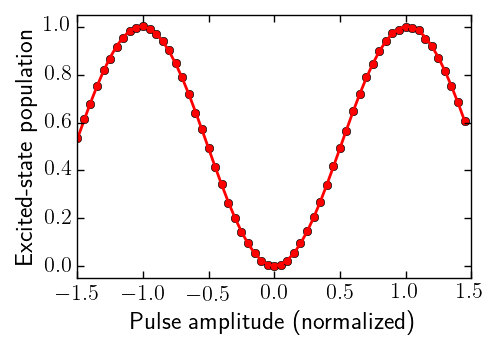
\includegraphics[width=\textwidth]{../Figures/Qubit characterization/Rabi.png}
          \end{center}
          \vspace{-20 pt}
          \caption{A Rabi measurement. In the center peak the pulse has zero amplitude, corresponding to the qubit being in the ground-state. The other two peaks therefore correspond to $X_{-\pi}$ and $X_\pi$ pulses, as the qubit is in the excited-state.}
          \label{fig:Rabi}
        \end{wrapfigure}

        Determining the correct amplitude for qubit gates is commonly performed using a Rabi measurement. In this measurement the amplitude of a pulse with rotation along the X-axis is varied monotonically. The pulse will cause the qubit to rotate at a Rabi rate $\Omega_R$, which is proportional to the pulse amplitude.

        After application of a pulse with Rabi rate $\Omega_R$ and duration $\tau$, the wavefunction of the qubit will be in state $\ket{\psi} = \cos{\left( \frac{\Omega_R}{2} \tau \right) } \ket{0} + \sin{\left( \frac{\Omega_R}{2} \tau \right)} \ket{1}$. During a subsequent measurement the qubit will be in the excited-state with probability $\sin^2{\left( \frac{\Omega_R}{2} \tau \right)}$ \cite{Reed}.

        In a Rabi measurement the amplitude is swept monotonically from a negative value to a positive value. The result should look like a cosine, as shown in Figure~\ref{fig:Rabi}. The center of this cosine is where the amplitude is zero, and therefore corresponds to the ground-state of the qubit. At the other peaks, where the deviation from the ground-state is maximal, the qubit is in the excited-state. The amplitude of the left peak corresponds to an $X_{-\pi}$ pulse, and the amplitude of the right peak to an $X_\pi$ pulse.

        \textbf{TODO:}
        \begin{itemize}
          \item Mention calibration points
        \end{itemize}

      \subsection{Qubit decoherence}
        Once the pulse amplitude has been calibrated the qubit state can be controlled. Ideally the state of a qubit remains fixed in the absence of pulses. However due to the qubit's interaction with its environment the qubit will experience decoherence. Decoherence can be viewed as the qubit experiencing random interactions with its environment, and as a result we lose information about the state of the qubit. The decoherence of the qubit can be characterized by its relaxation time $T_1$, and its dephasing time $T_2$.

        \subsubsection{Qubit relaxation: $T_1$}

          \begin{wrapfigure}[9]{r}{0.3\textwidth}
            \begin{center}
            \vspace{-30pt}
              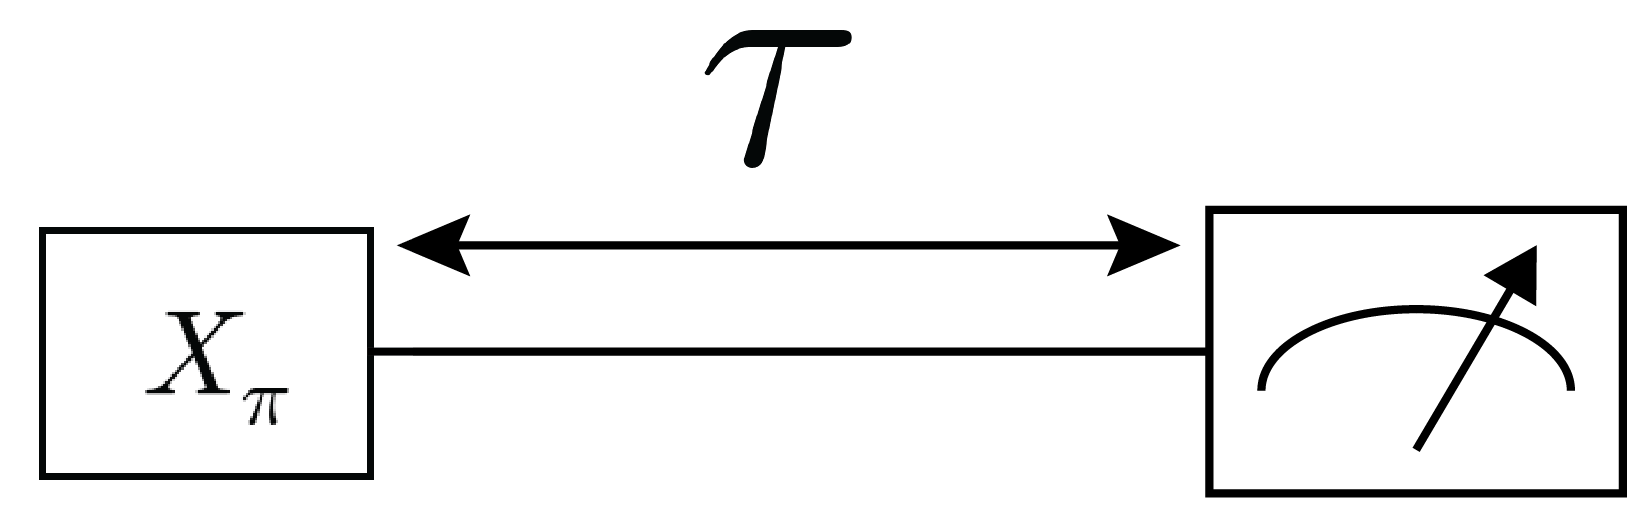
\includegraphics[width=\textwidth]{../Figures/Qubit characterization/T1 decoherence.png}
            \end{center}
            \vspace{-20 pt}
            \caption{Schematic of a T1 sequence. An $X_\pi$ pulse is applied to the qubit, and after a waiting time $\tau$ the qubit is measured.}
            \label{fig:T1 schematic}
          \end{wrapfigure}

          One type of decoherence is relaxation, which results in the excitation of the qubit slowly leaking away to its environment through different relaxation channels. Some of these relaxation channels have been discussed in \ref{sec:Losses}. The relaxation can be measured in a $T_1$-measurement, a schematic of which is shown in Figure~\ref{fig:T1 schematic}. In a $T_1$-measurement an initial pi-pulse is applied, after which the qubit is in its excited state. After waiting for a monotonically increasing wait time $\tau$, the state of the qubit is measured. During the wait time $\tau$ the qubit experiences an exponential decay due to relaxation, with a corresponding decay time $T_1$.

          \begin{itemize}
            \item Purcell limit
          \end{itemize}

        \subsubsection{Qubit dephasing: Ramsey}
          \label{sssec:Ramsey}

          \begin{wrapfigure}[8]{r}{0.4\textwidth}
            \begin{center}
            \vspace{-30pt}
              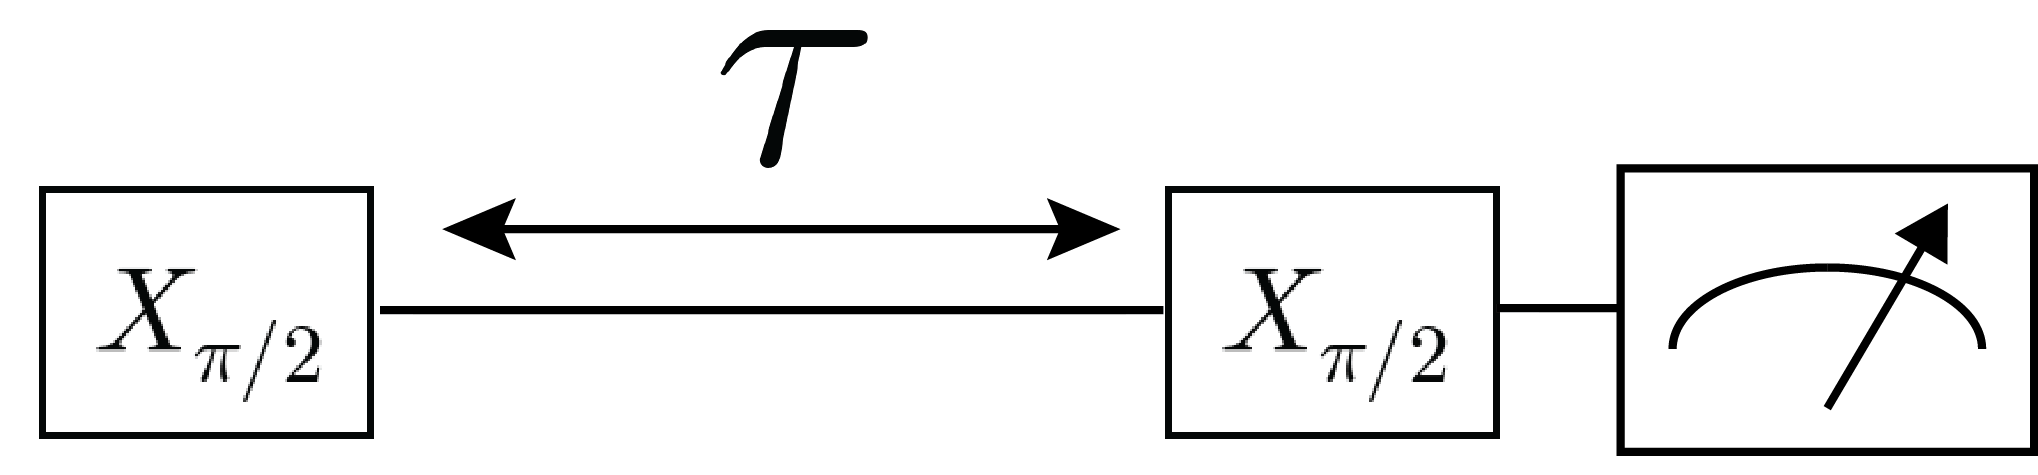
\includegraphics[width=\textwidth]{../Figures/Qubit characterization/T2 decoherence.png}
            \end{center}
            \vspace{-20 pt}
            \caption{Schematic of a $T_2^*$ sequence.}
            \label{fig:T2star schematic}
          \end{wrapfigure}

          Aside from relaxation, the qubit also experiences dephasing, resulting from phase noise. Phase noise can be seen as fluctuations in the qubit frequency, and results in a random phase being added to the qubit. It can be visualized on the Bloch sphere as the transversal component of the qubit's state decreasing in magnitude, as the qubit's phase has increased uncertainty. In the limiting case this will result in all phase information being lost, with the qubit's state thereby lying on the Z-axis.

          The amount of dephasing is characterized by the dephasing time $T_2^*$, which has an upper bound equal to $2\;T_1$ due to dissipation \cite[pp56-58]{Bishop}. However it can decrease significantly due to other sources of phase noise, such as charge noise, fluctuating cavity photon number, and flux noise for flux-tunable qubits \cite[p126]{Sears}.

          Measuring the dephasing time $T_2^*$ is done in a Ramsey measurement, a schematic of which is shown in Figure~\ref{fig:T2star schematic}. A Ramsey sequence consists of an initial $X_{\pi/2}$ pulse, after which the qubit lies on the equator of the Bloch sphere. After a certain wait time $\tau$, a second $X_{\pi/2}$ pulse is applied to the qubit. The combination of the two pulses should result in the qubit ending up at the excited-state. However, during the wait time $\tau$ the qubit experiences dephasing, causing it to deviate from its original position on the equator. Therefore the final state of the qubit will deviate from the qubit's excited-state. The probability of the final state to end up in the excited-state has an exponential decay, asymptotically approaching $0.5$ (all phase information lost).

          During the wait time $\tau$, when the qubit lies on the equator, it does not only experience dephasing. When the frequency of the driving tone $\omega_d$ is different from the qubit frequency $\omega_q$, the qubit will precess along the equator with a frequency equal to the frequency difference $\omega_d - \omega_q$. Due to this precession the Ramsey measurement also exhibits an oscillation. The frequency of the oscillation can in fact be used to accurately determine the qubit frequency (see Section~\ref{sec:Accurate frequency estimation}).

        \subsubsection{Fast frequency qubit dephasing: Echo}

          \begin{wrapfigure}[8]{r}{0.4\textwidth}
            \begin{center}
            \vspace{-30pt}
              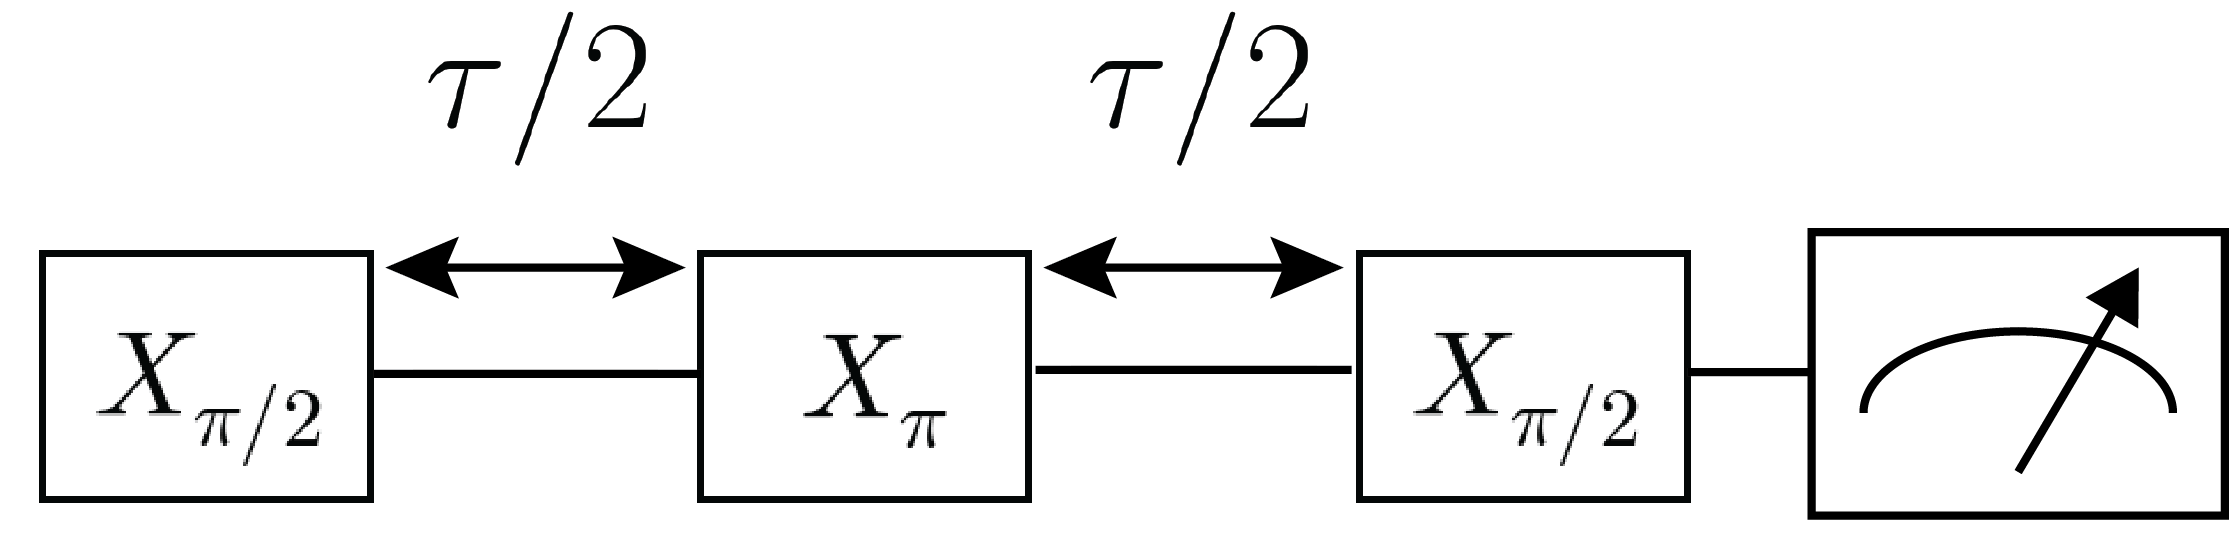
\includegraphics[width=\textwidth]{../Figures/Qubit characterization/T2echo decoherence.png}
            \end{center}
            \vspace{-20 pt}
            \caption{Schematic of a $T_2^E$ sequence.}
            \label{fig:T2echo schematic}
          \end{wrapfigure}

          The dephasing time $T_2^*$ is a combination of several different phase noise sources. Some of these sources produces high frequency (fast) noise, while others produce low frequency (slow) noise. It is possible to distinguish these two effects by performing a second dephasing measurements that filters out slow noise, called an Echo measurement, and its schematic is shown in Figure~\ref{fig:T2echo schematic}.

          An Echo measurement is quite similar to a Ramsey measurements, where two $X_{\pi/2}$ pulses are applied, separated by a wait time $\tau$. The difference is that in the middle of this wait time, at $\tau/2$, an additional refocusing $X_{\pi}$ pulse is sent. The refocusing pulse flips the qubit state on the Bloch sphere around the X-axis. Any slow phase noise, which we can view to be quasi-static, is thereby cancelled. Fast phase noise, however, will vary considerably during the wait time $\tau$, and so will still cause dephasing. In the absence of decoherence, the final state of the qubit is the ground-state, which is in contrast to a Ramsey measurement, where the final state is the excited-state.

          An Echo measurement is performed by monotonically increasing the wait-time $\tau$, while keeping the three pulses relative to the wait time $\tau$ fixed. The result is similar to a Ramsey measurement, showing an exponential decay, with corresponding Echo dephasing time $T_2^E$. This value should be higher or equal to the dephasing time $T_2^*$. The refocusing pulse has the additional effect that any precession due to detuning is also cancelled, thereby inhibiting the oscillatory behaviour that is present in Ramsey measurements. To be able to better estimate the Echo dephasing time $T_2^E$, the phase of the final $X_{\pi/2}$ pulse is monotonically shifted, resulting in an artificial oscillation.

      \subsection{Second excited-state}
        \label{ssec:Second excited-state}

        \begin{wrapfigure}[15]{r}{0.4\textwidth}
          \begin{center}
          \vspace{-30pt}
            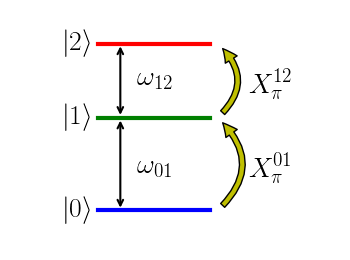
\includegraphics[width=\textwidth]{../Figures/Exploring frequency re-use/schematic second transition pulsing.png}
          \end{center}
          \vspace{-20 pt}
          \caption{Schematic of the pulse combination used to reach the second excited-state. First an $X_\pi^{01}$-pulse is applied at frequency $\omega_{01}$. Secondly an $X_\pi^{12}$-pulse is applied at frequency $\omega_{12}$ such that the transmon is in its second excited-state.}
          \label{fig:schematic pulsing to second excited-state}
        \end{wrapfigure}

        When viewing the transmon as a qubit the higher energy levels are neglected. However, qubit pulses may result in some population leakage to the second excited-state. This is especially the case when the pulse length is short and when the DRAG parameter is not well-calibrated (see Section~\ref{ssec:DRAG parameter calibration} for information on the DRAG pulse). Measuring the population in the second-excited state due to leakage requires being able to excite the transmon to its second excited-state. This can be done by first exciting the transmon to its first excited-state, and then applying a second pulse at the second transition frequency of the transmon, as shown in Figure~\ref{fig:schematic pulsing to second excited-state}. Measuring this frequency has been explained in Section~\ref{ssec:12-transition spectroscopy}.

        Determining the correct amplitude for the pulse at the second transition frequency can be done using a second transition Rabi measurement, where an initial $X_\pi$-pulse is applied to excite the transmon to its first excited-state. The amplitude of the second pulse is varied from negative to positive, similar to a standard Rabi measurement. Optionally a third $X_\pi$-pulse at the first transition frequency of the transmon. The third pulse transfers any remaining excitation in the first excited-state back to the ground-state.

        \begin{wrapfigure}[18]{r}{0.4\textwidth}
          \begin{center}
          \vspace{-30pt}
            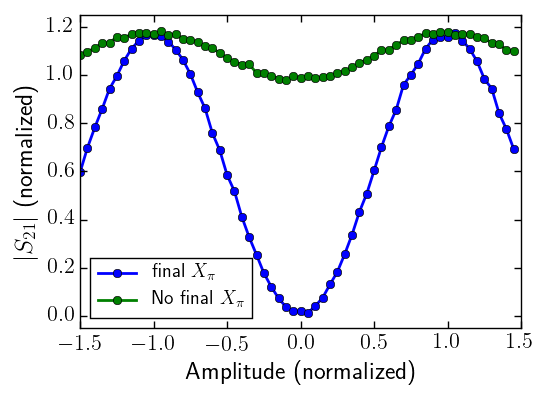
\includegraphics[width=\textwidth]{../Figures/Qubit characterization/Rabi12.png}
          \end{center}
          \vspace{-20 pt}
          \caption{A second transition Rabi measurement of the second excited-state, both with and without final $X_\pi$ pulse. The signal is rotated and normalized such that $\left|S_{21}\right|=0$ corresponds to the transmon in the ground-state, and $\left|S_{21}\right|=1$ corresponds to the transmon in the first excited-state.}
          \label{fig:Rabi12}
        \end{wrapfigure}

        The pulse-amplitude required to pulse to the second excited-state has been calibrated for both the top and bottom qubit. In Figure~\ref{fig:Rabi12} a second transition Rabi measurement is shown for the top qubit. The measurement is performed both with and without a third $X_\pi$ pulse. As can be seen the signal reaches above the signal of the first excited-state, and so it can be concluded that the second-excited state is indeed populated. Furthermore, since the signal at the second excited-state peaks are identical for the measurements with and without the final pulse, it can be concluded that at these amplitudes there is no residual excitation in the first excited-state, and that indeed the transmon is fully excited to the second excited-state.


    \section{Exploring Frequency re-use}
      \label{sec:Exploring Frequency re-use}
      \begin{figure}[tb]
        \centering
        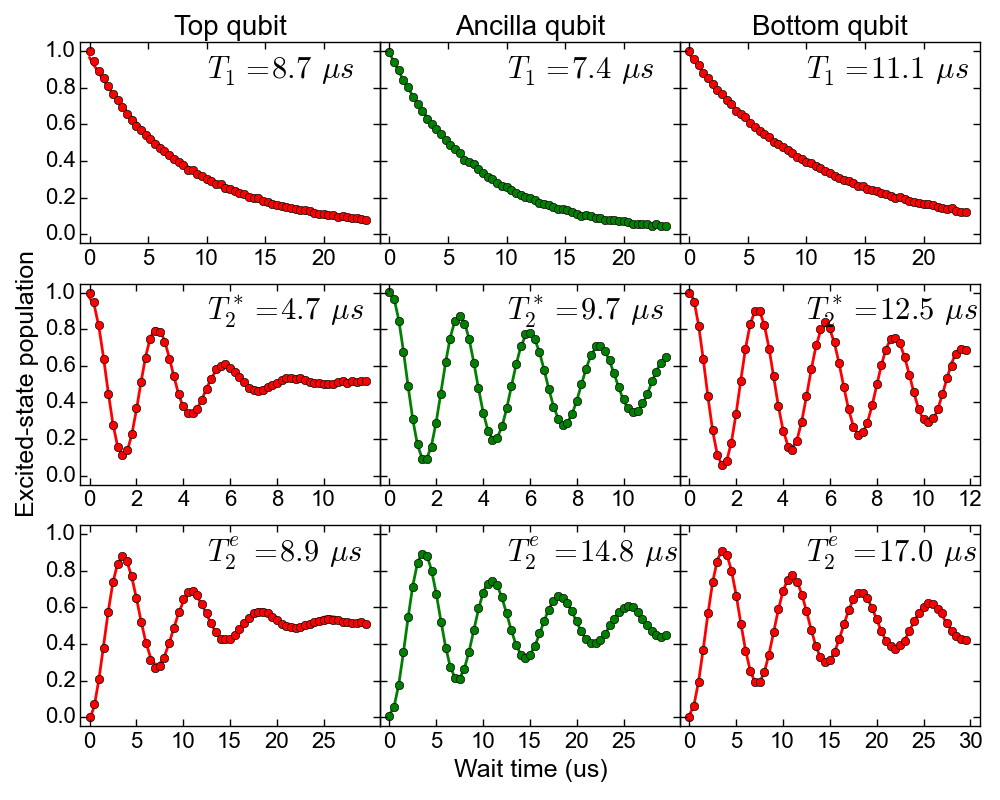
\includegraphics[width=\linewidth]{../Figures/Exploring frequency re-use/coherence_times.png}
        \caption{Decoherence times of the three qubits in Muxmon0. The top qubit frequency is tuned to match the bottom qubit frequency (\SI{6.22}{\giga \hertz}). When measuring the coherence times of either the top or bottom qubit the other qubit was detuned by \SI{50}{\mega \hertz} to suppress cross-coupling effects. The fit for the dephasing time $T_2^*$ of the top qubit was performed using a Gaussian noise model.}
        \label{fig:decoherence times Muxmon0}
      \end{figure}

      \begin{table}
        \begin{tabular}{l c c}
          \toprule
          Qubit  & $f_\text{max}$ (GHz) & $f_\text{res}$ (GHz)\\
          \midrule
          Top    & 6.277                & 6.700 \\
          Ancilla& 6.551                & 6.733 \\
          Bottom & 6.220                & 6.800 \\
          \bottomrule
        \end{tabular}
        \caption{Sweet-spot frequencies $f_\text{max}$, and resonator frequencies $f_\text{res}$ of the three qubits in the Muxmon0 chip}
        \label{tab:Muxmon0 qubit properties}
      \end{table}

      The frequencies of the qubits and their corresponding resonators are shown in Table~\ref{tab:Muxmon0 qubit properties}. The resonator buses have a frequency of \SI{4.88}{\giga \hertz} and \SI{4.97}{\giga \hertz} for the bus connecting the ancilla qubit to the top and bottom qubit respectively (see Appendix~\ref{sec:Resonator buses}).

      To study frequency re-use, the top qubit frequency has been tuned to that of the bottom qubit, while the ancilla and bottom qubits were kept at their respective sweet-spots. Under these conditions the decoherence times of the three qubits are shown in Figure~\ref{fig:decoherence times Muxmon0}. The dephasing time $T_2^*$ of the top qubit is considerably lower than of the ancilla and bottom qubit. The reason is that the top qubit is tuned away from its sweet-spot to match the frequency of the bottom qubit. As a result its frequency response to flux is higher, and so it is more susceptible to flux noise.

      Having the top and bottom qubit at the same frequency gives rise to cross-coupling and cross-driving effects. It is important to characterize these effects, as they can potentially result in gate errors.

    \subsection{Cross-coupling}
      \label{ssec:cross-coupling}
      \begin{figure}[tb]
        \centering
        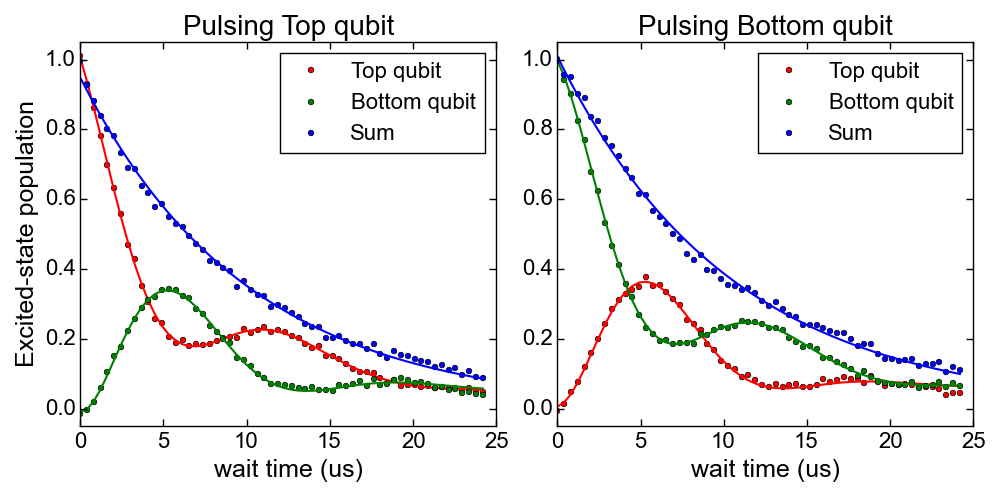
\includegraphics[width=\linewidth]{../Figures/Exploring frequency re-use/excitation_swap.png}
        \caption{After initially exciting one qubit, and measuring the excited-state population of both qubits versus time, an excitation swap is observed. The extracted coupling strength is equal to $J2\pi=72.0 \pm 1.8$ kHz}
        \label{fig:excitation swap}
      \end{figure}

      The top qubit is coupled to the botom qubit via the following three successive components:

      \begin{enumerate}
        \item The resonator bus coupling the top qubit to the ancilla qubit.
        \item The ancilla qubit.
        \item The resonator bus coupling the two ancilla qubit to the bottom qubit.
      \end{enumerate}

      When the top and bottom qubit are tuned into resonance, the two qubits experience an exchange interaction. This interaction leads to an excitation in one qubit being able to transfer to the other qubit. This can result in the swapping of excitation between the top and bottom qubit, at a rate given by the interaction strength $J$. The excitation swapping of the top and bottom qubit when tuned into resonance can be seen in Figure~\ref{fig:excitation swap}. From these results the coupling $J$ is found to be equal to $J/2\pi=72. \pm 1.8$ kHz. For more information on the exchange interaction see section~4.3.2 of the thesis by Chow \cite{Chow}.

    \subsection{Cross-driving}
      \label{ssec:cross-driving}

      \begin{figure}[tb]
        \centering
        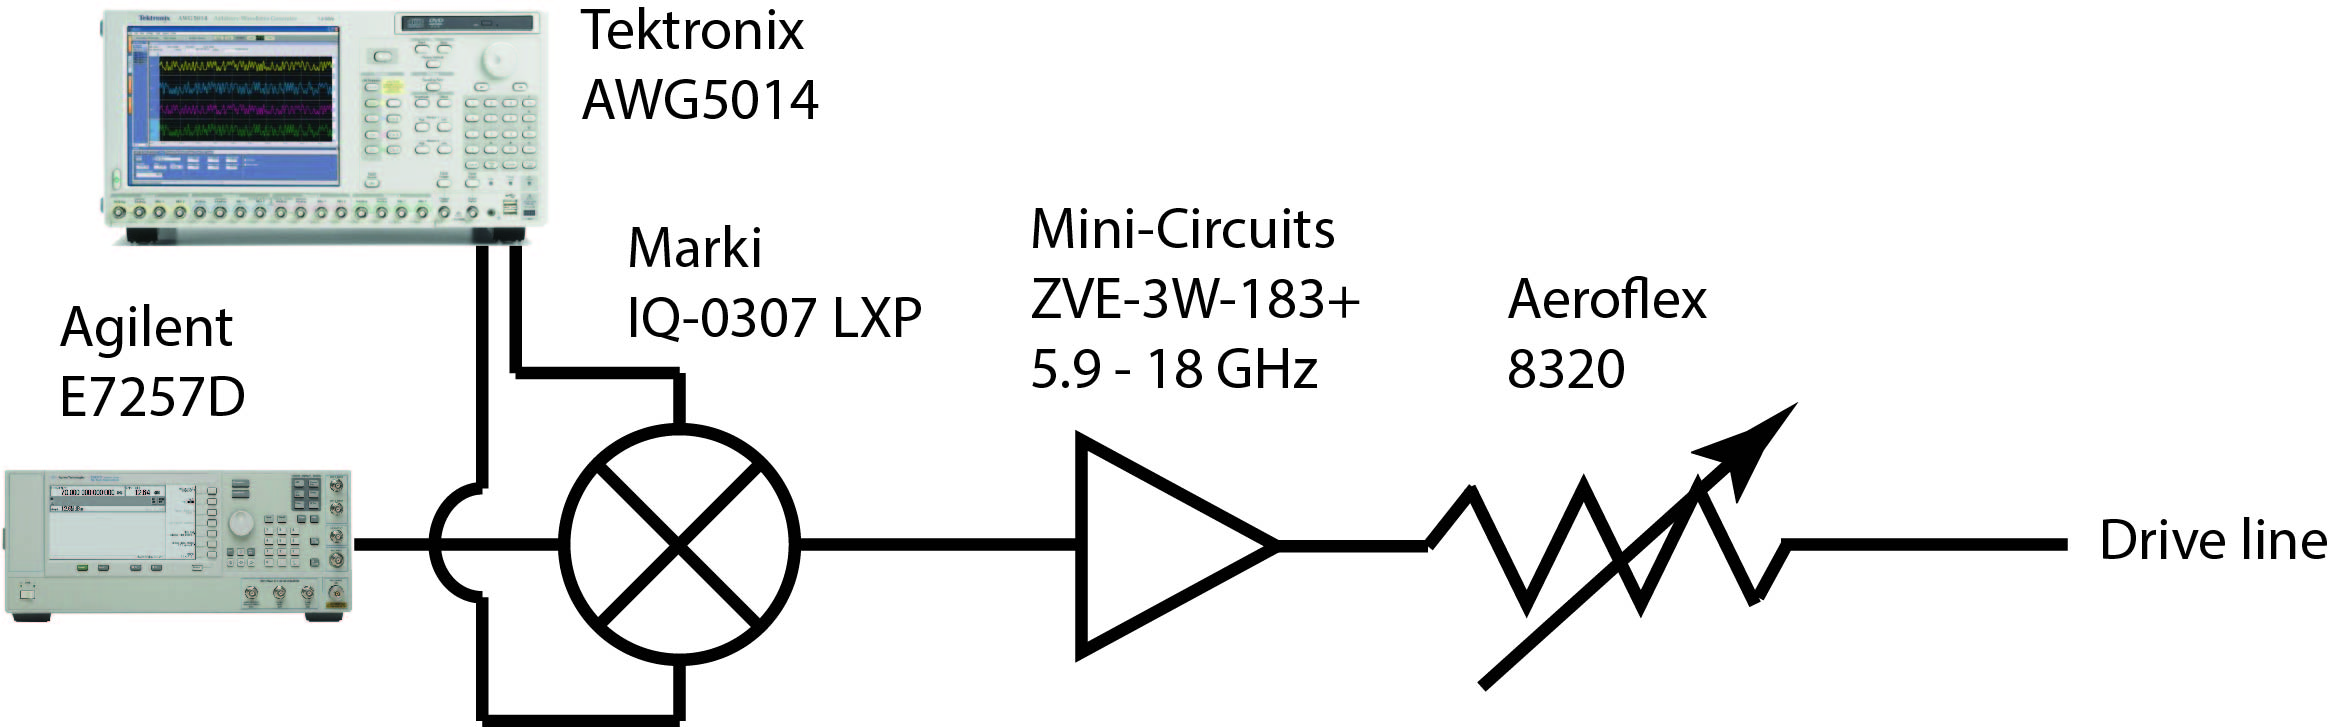
\includegraphics[width=.8\textwidth]{../Figures/Exploring frequency re-use/cross-driving_setup.jpg}
        \caption{Schematic for measuring the amount of cross-driving using the direct drive lines of the top and bottom qubit. The combination of amplifier and variable attenuator allow a range range of drive strengths.}
        \label{fig:cross-driving schematic}
      \end{figure}

      \begin{figure}[tb]
        \centering
        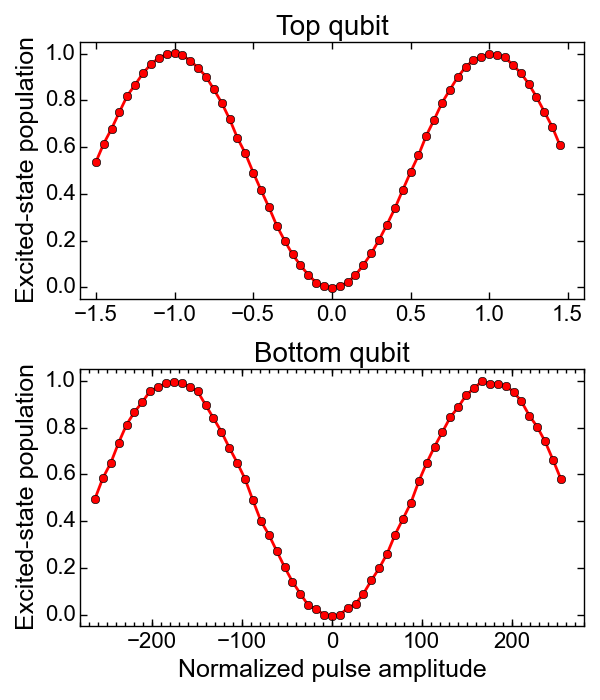
\includegraphics[width=.5\textwidth]{../Figures/Exploring frequency re-use/cross-driving_Rabi.png}
        \captionof{figure}{Required drive amplitude required to drive the top and bottom qubit through the top qubit drive line. The amplitude has been normalize to the amplitude required for a pi pulse on the top qubit.}
        \label{fig:cross-driving Rabi}
      \end{figure}
      \begin{table}
        \begin{tabular}{l c c}
          \toprule
          qubit & \multicolumn{2}{c}{cross-driving (\%)} \\
          \cmidrule(lr){2-3}
               & top drive line & bottom drive line \\
          \midrule
          Top     & $-$    & $0.23$ \\
          Ancilla & $0.79$ & $0.66$ \\
          Bottom  & $0.57$ & $-$    \\
          \bottomrule
        \end{tabular}
        \label{tab:cross-driving}
      \end{table}
        % \captionof{table}{Driving through top qubit drive line}
        %   \vspace{2cm}
        %   \begin{tabular}{l c}
        %     \toprule
        %     qubit & cross-driving (\%) \\
        %     \midrule
        %     Top & $0.23$ \\
        %     Ancilla &$ 0.66$ \\
        %     Bottom & $-$ \\
        %     \bottomrule
        %   \end{tabular}
        %   \captionof{table}{Driving through bottom qubit drive line}
        %   \label{tab:cross-driving bottom}
        % \end{minipage}

      When driving one of the qubits through its dedicated drive line, the signal can partially leak through to the other qubits. The cause of this leakage may be on-chip, where the components separating the qubits do not fully filter the signal, or may be off-chip, due to for instance imperfect isolation between the cables or other components. This signal leakage results in cross-driving effect, where driving one qubit will also partially drive the other qubits. Cross-driving effects affect the performance of the qubits when the frequency of the driven qubit and the cross-driven qubit are in resonance, as is the case with the Muxmon experiment.

      The amount of cross-driving can be determined by measuring the pulse amplitude required to drive each of the three qubits through a drive line. The cross-driving due to the finite isolation of the Duplexer has been separately measured (see Appendix~\ref{ch:Duplexer isolation}). At the frequencies used in the experiment, the isolation of the Duplexer was found to be typically around \SI{50}{\dBm}. The amount of cross-driving due to other sources was determined by measuring the pulse amplitude required to perform a Rabi on each of the qubits using a fixed drive line. The measurements were performed using the set-up shown in Figure~\ref{fig:cross-driving schematic}. The results of a single cross-driving measurement is shown in Figure~\ref{fig:cross-driving Rabi}, where the top and bottom qubit are driven through the drive line of the top qubit. The pulse amplitude is normalized to the amplitude required for applying pi pulse to the qubit directly connected to the drive line. The amount of cross-driving is equal to the ratio of the pulse amplitude required for a pi rotation for the main qubit, and for the cross-driven qubit. The cross-driving ratio's are shown in Tables~\ref{tab:cross-driving top} and ~\ref{tab:cross-driving bottom}. The cross-driving ratio's are found to be less than one percent, and are higher for the ancilla qubit than for the other cross-driven qubit. This indicates that the main source of cross-driving is likely on-chip. Furthermore it can be seen that the cross-driving is stronger from the drive line of the top qubit than from the drive line of the bottom qubit.

      \begin{wrapfigure}[12]{r}{0.45\textwidth}
        \begin{center}
        \vspace{-30pt}
          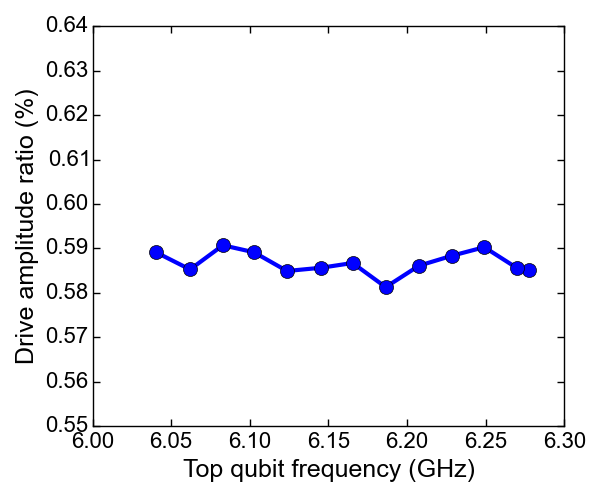
\includegraphics[width=\textwidth]{../Figures/Exploring frequency re-use/cross-driving_vs_top_frequency.png}
        \end{center}
        \vspace{-20 pt}
        \caption{Cross-driving ratio of the bottom qubit when pulsing from the drive line of the top qubit, versus frequency of the top qubit. }
        \label{fig:cross-driving versus top frequency}
      \end{wrapfigure}

      As a check that the effects observed are indeed due to cross-driving, and not due to cross-coupling, the cross-driving when driving the bottom qubit through the drive line of the top qubit has been measured as the frequency of the top qubit is varied. The results are shown in Figure~\ref{fig:cross-driving versus top frequency}. If the effect is due to cross-coupling the amount of cross-driving should depend strongly on the detuning between the top qubit and bottom qubit. Instead we see that the cross-driving is approximately constant, indicating that this is indeed a cross-driving effect instead of a cross-coupling effect.


    \textbf{Figures that need to be included:}
    \begin{itemize}
      \item schematic of cross-coupling and readout cross-talk \\
          It could be good to create this using the actual Muxmon chip as background, with arrows indicating how the different effects operate
    \end{itemize}



  \chapter{Calibration routines}
    \label{ch:Calibration routines}
    \textbf{TODO:} Introduction

    \section{Qubit calibrations}
      \label{Qubit calibrations}

      \subsection{Accurate frequency estimation}
        \label{ssec:Accurate frequency estimation}
        Spectroscopy provides an estimate for the frequency of the qubit. However, even with pulsed spectroscopy, the accuracy is limited to about \SI{1}{\mega \hertz}. As explained in Section~\ref{sssec:Ramsey}, any difference between a drive frequency $\omega_d$ and qubit frequency $\omega_q$ will result in the qubit precessing around the Z-axis.

        In a Ramsey measurement this precession can be measured, from which the qubit frequency can be inferred. This provides a very accurate estimate for the qubit frequency $\omega_q$. The longer the wait time $\tau$, the more the qubit precesses around the equator. Small differences between the drive frequency $\omega_\text{drive}$ and the qubit frequency $\omega_q$ can be detected. The upper bound on the accuracy of being able to determine the qubit frequency is set by the qubit's dephasing time $T_2^*$, because it corresponds to the inherent fluctuation in the qubit frequency.

        The main goal of the Muxmon experiment is to determine the performance of selective broadcasting combined with frequency re-use, which requires the top and bottom qubit to be at the same frequency. Any effect due to weak coupling between the qubits is only present if the two qubits are accurately tuned to the same frequency. Furthermore, any frequency detuning from the drive frequency $\omega_d$ will lead to a decrease in qubit performance. The top qubit frequency was initially tuned using spectroscopy. Accurate frequency tuning was then performed using Ramsey measurements. The bottom qubit frequency $\omega_q^B$ was first determined, after which the top qubit frequency $\omega_q^T$  was tuned to match $\omega_q^B$. Using Ramsey measurements the inidividual frequencies could be determined to within \SI{10}{\kilo \hertz}, and the two frequencies could be tuned to within \SI{50}{\kilo \hertz} of one another. The limit to tuning the frequencies was not determined by the Ramsey measurement accuracy, but due to the IVVI having a finite DAC voltage stepsize.

      \subsection{Accurate drive amplitude calibration}
        \label{ssec:PiX360}
        To test the limits of performance using the Duplexer all gates need to be calibrated to a very high accuracy. The Rabi measurement explained in section~\ref{ssec:Rabi} is able to tune the drive amplitude up to a certain degree. However, the degree to which one can tune the drive amplitude using Rabi is limited, and for fine-tuning different methods are required.

        \begin{figure}[tb]
          \centering
          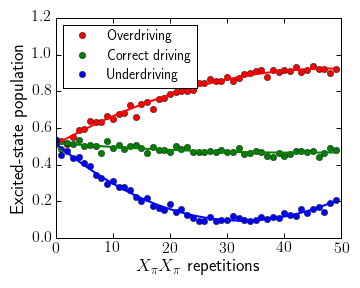
\includegraphics[width=.6\linewidth]{../Figures/Calibration routines/Drive calibration.png}
          \caption{Accurate drive calibration using repeated pi-pulses. The initial slope determines if the system is overdriving (positive slope), or underdriving (negative slope)}
          \label{fig:PiX360}
        \end{figure}

        In the Muxmon experiment, the method used for accurate drive amplitude calibration is based on applying repeated pi-pulses on the qubit. The entire sequence can be summarized as $\left( X_{\pi} \right)^{2N} X_{\pi/2} \ket{0}$, where $N$ is the segment number. In the absence of gate errors and decoherence, the qubit should return to the equator, regardless of the segment number $N$. However, any amount of overdriving or underdriving results in small rotations that are added coherently, resulting in a positive or negative slope respectively. These slopes serve as very accurate measures for the optimal drive amplitude. Three such examples are shown in Figure~\ref{fig:PiX360}. If the difference in driving strength is large, oscillations will be present, corresponding to rotations around the Bloch sphere.

      \subsection{DRAG parameter calibration}
        \label{ssec:DRAG parameter calibration}

        Ideally a transmon has two energy levels, and so can be treated as a qubit. However, in Section~\ref{sec:resonator-scan} it was shown that the degree to which we can ignore the second excited-state depends on the anharmonicity $\alpha=\omega_{12} - \omega_{01}$.  The presence of the second excited-state (and to lesser extent higher excited-states) can have a considerable influence on the gate performance in two different ways. First of all gates can cause a direct excitation into the second excited-state, thereby resulting in leakage outside the qubit two-state Hilbert space. Ensuring that the frequency bandwidth corresonding to the gate is small compared to the anharmonicity $\alpha$ can greatly reduce this leakage. However, an additional form of leakage is manifested as a virtual excitation to the second excited-state during the pulse, resulting in an added phase error.

        \begin{wrapfigure}[12]{r}{0.5\textwidth}
          \begin{center}
          \vspace{-30pt}
            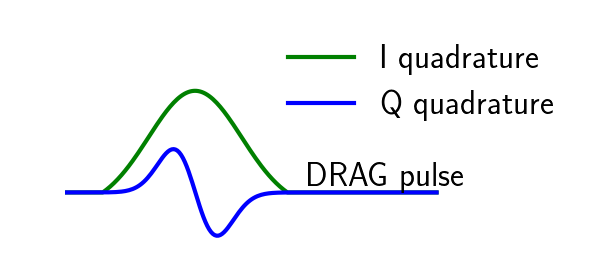
\includegraphics[width=\textwidth]{../Figures/Exploring frequency re-use/DRAG pulse.png}
          \end{center}
          \vspace{-20 pt}
          \caption{Schematic representation of the DRAG pulse. The I quadrature pulse is the main Gaussian pulse, while the Q quadrature pulse is the derivative of the Gaussian.}
          \label{fig:DRAG pulse}
        \end{wrapfigure}

        A modification to the Gaussian, known as the Derivative Removal by Adiabatic Gate (DRAG) pulse \cite{motzoi2009simple}, can be used to suppress leakage errors. The DRAG pulse relies on quadrature control, where one quadrature consists ofthe main Gaussian pulse, while the quadrature consists of the derivative of the main Gaussian pulse. The DRAG pulse can reduce leakage and virtual excitation-induced phase errors by roughly an order of magnitude. The DRAG pulse is shown in Figure~\ref{fig:DRAG pulse}.

        The DRAG parameter is the relative amplitude between the derivative pulse and the main Gaussian pulse, and must be accurately calibrated. It has been shown that the virtual excitation-induced phase error is present up to first order in a pi/2-pulse~\cite{lucero2010reduced}. In the Muxmon experiment the DRAG parameter has been calibrated using a method suggested by Reed~\cite{Reed}, by measuring the difference in signal between an $X_{\pi} Y_{\pi/2}$ pulse and a $Y_{\pi} X_{\pi/2}$ pulse. Ideally for both pulses the final state should lie on the equator. However, any phase error would result in these two measurement shifting away from the equator in opposite direction. The DRAG parameter is found by minimizing this difference.

      \subsection{AllXY}
        \label{ssec:AllXY}
        There is a good measurement to test how well the qubit has been tuned. It is known as the AlllXY measurement, and consists of all 21 possible two-gate combinations of $\left\{Id, X_{\pi}, Y_{\pi}, X_{\pi/2}, Y_{\pi/2}\right\}$. Each combination is susceptible to different types of gate errors to a different degree. The AllXY combinations have therefore been arranged in such a way that the final state of the first five combinations is the ground-state, the final state of the second twelve combinatios is the equator, and the final state of the last four combinations is the excited-state. Furthermore the combinations are arranged in such a way that the most common sources of gate errors can be distinguished. The full list of combinations in correct order can be found in Appendix~\ref{ssec:AllXY app}.

        The errors that can be distinguished are extensive: drive amplitude, DRAG parameter, frequency detuning, signal reflections, and several more. This is the strength of AllXY, but simultaneously its weakness. If there are multiple errors present, their errors may interfere, resulting in symptoms which are difficult to diagnose. nevertheless, it is a powerful tool, especially if one source of gate error is dominant. For a detailed analysis of the AllXY symptoms produced by different types of gate errors, see Reef~\cite{Reed}.

        The Duplexer can modify the signal of each of its input-output port combinations individually. In the set-up used for the Muxmon experiment, both the drive amplitude and DRAG parameter can be separately tuned for each of the two qubits. In Figure~\ref{fig:AllXY individual control} the AllXY results are shown for the top and bottom qubits, as either the drive amplitude or DRAG parameter of the top qubit is varied using the Duplexer. As can be seen there is no noticeable change in the AllXY of the bottom qubit, even though the top qubit's performance changes considerably. This shows that the Duplexer allows for individual drive amplitude and DRAG parameter control for each qubit, without affecting the other.

        \begin{figure}
        \centering
           \begin{subfigure}[b]{\textwidth}
           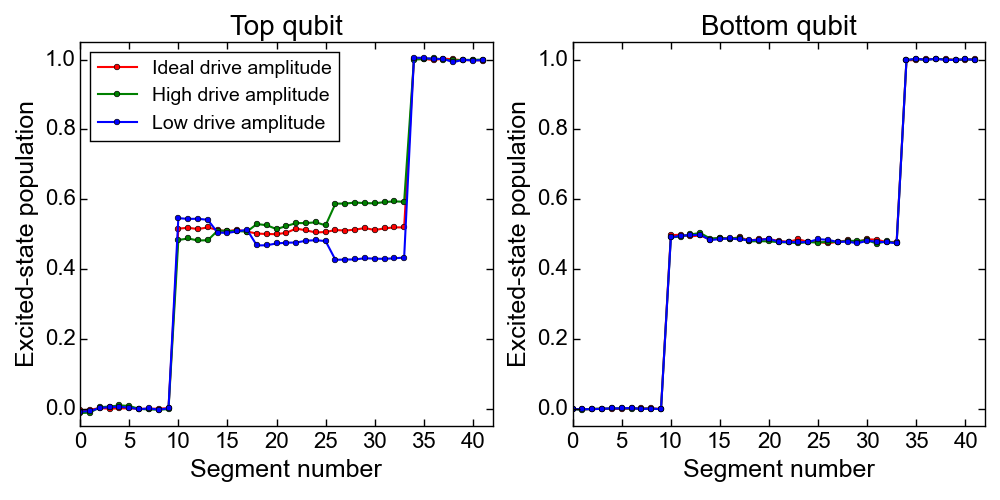
\includegraphics[width=1\linewidth]{../Figures/Exploring frequency re-use/AllXY_drive_top.png}
           \caption{}
           \label{fig:AllXY drive top}
        \end{subfigure}

        \begin{subfigure}[b]{\textwidth}
           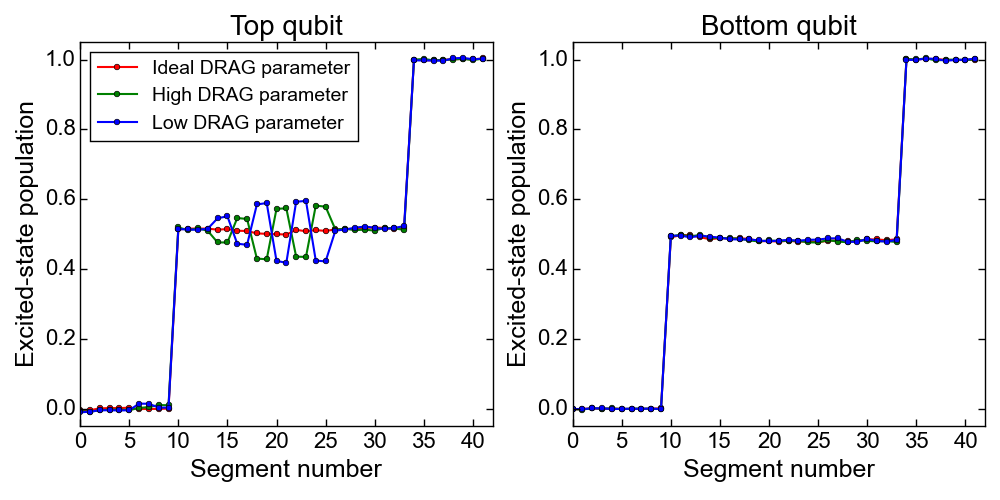
\includegraphics[width=1\linewidth]{../Figures/Exploring frequency re-use/AllXY_drag_top.png}
           \caption{}
           \label{fig:AllXY DRAG top}
        \end{subfigure}

        \caption[Two numerical solutions]{AllXY measurement of the top and bottom qubit as one parameter of the top qubit is varied. The parameter varied is (a) drive amplitude, (b) DRAG amplitude. The AllXY sequences are placed on top of each other. As can be seen the bottom qubit has no noticeable change in the AllXY measurements when the parameters of the top qubit are varied.}
        \label{fig:AllXY individual control}
        \end{figure}

    \section{Instrument calibrations}
      \label{Instrument calibrations}

      \subsection{IQ mixer calibration}
        \label{ssec:Mixer calibration}

        \begin{figure}[tb]
          \centering
          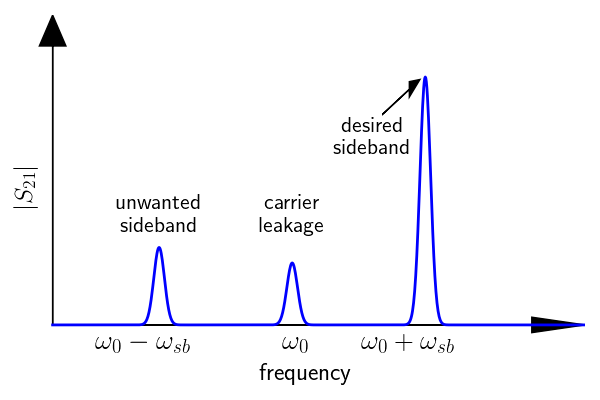
\includegraphics[width=.7\textwidth]{../Figures/Calibration routines/Mixer leakage schematic.png}
          \caption{Schematic showing spurious signals resulting from mixer leakage and mixer skewness,when using single sideband modulation with frequency $\omega_{sb}$.}
          \label{fig:mixer imperfections schematic}
        \end{figure}

        \begin{figure}[tb]
          \centering
          \begin{subfigure}[h]{0.49\textwidth}
            \caption{}
            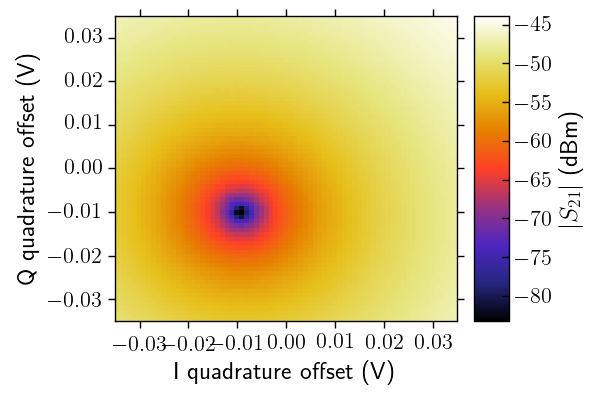
\includegraphics[width=\textwidth]{../Figures/Calibration routines/Mixer offset.png}
          \end{subfigure}
          \begin{subfigure}[h]{0.49\textwidth}
            \caption{}
            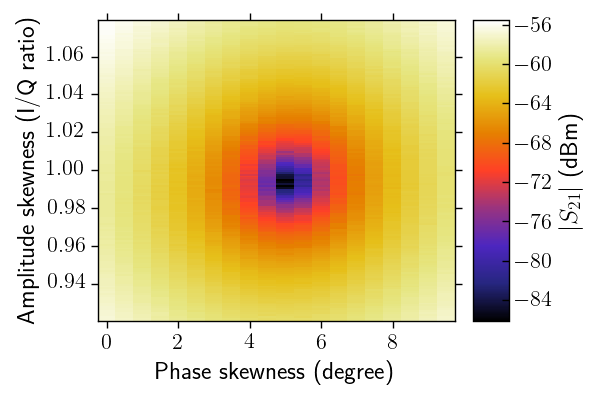
\includegraphics[width=\textwidth]{../Figures/Calibration routines/Mixer skewness.png}
          \end{subfigure}
          \caption{Mixer carrier leakage (a) and mixer skewness (b). Without any corrections both the mixer carrier leakage and the signal due to mixer skewness are equal to \SI{-58}{\dBm}. Compared to the main signal with output power equal to \SI{-32}{\dBm}, the mixer imperfections would result in two additional signals, each with strength \SI{-26}{\dB}.}
          \label{fig:Mixer calibrations 2D}
        \end{figure}

        An important calibration routine which must not be forgotten is correcting for mixer imperfections. An IQ mixer must be calibrated for two types of mixer imperfections: the mixer carrier leakage, and the mixer skewness. These imperfections result in two spurious signals, which are shown in Figure~\ref{fig:mixer imperfections schematic}.

        For a perfectly balanced mixer, a signal of given frequency $\omega_0$ at the LO port should produce no output at the RF port if no modulation signal is applied in the inphase and quadrature ports.  However, any imperfections, due to for instance diode mismatches in the mixer, may lead to some signal at frequency $\omega_0$ leaking through. This leakage can be compensated to a large extent by adding a DC offset to the inphase and quadrature IF signals leaving the AWG, for which the leakage is minimized. Determining the optimal DC offset can be performed by sending a carrier signal into the LO port of the mixer, and a continuous DC signal from the AWG to both IF ports of the mixer. The leakage can be measured as signal exiting the RF port at the carrier frequency $\omega_0$, and can be minimized by varying the offsets of the individual AWG channels.

        Another type of IQ mixer imperfection is mixer skewness. The carrier signal entering the LO port is split into its inphase and quadrature component, where it is mixed with an inphase and quadrature IF signal. Ideally the inphase and quadrature components of the LO signal are perfectly orthogonal. However, in reality this is not the case, and so a small amount of skewness is present. Ideally the signal should be shifted in frequency to the desired sideband frequency $\omega_0 + \omega_{sb}$. However, any mixer skewness will lead to the signal being partially shifted in the opposite direction, resulting in some signal at the unwanted sideband frequency $\omega_0 - \omega_{sb}$. Additionally any amplitude skewness between the two IF ports will also result in signal at the unwanted sideband frequency. The signal at the unwanted sideband can be measured for a given carrier frequency $\omega_0$ by adding a sine and cosine with sideband frequency $\omega_{sb}$ to the inphase and quadrature ports respectively.   This can be corrected during the generation of the pulses through a transformation $\left( I, Q \right) \rightarrow \left( I', Q' \right) = \left( I - Q \tan{\phi}, Q \sec{\phi} \right)$, where $\phi$ is the phase skewness. The skewness can be corrected by varying the phase and amplitude of one of the AWG channels, and minimizing the signal at the unwanted sideband. The inphase and quadrature signals have to be transformed for every phase. Note that the mixer skewness is dependent on both the carrier frequency $\omega_0$ and the sideband modulation frequency $\omega_{sb}$

      \subsection{Duplexer phase calibration}
        \label{ssec:Duplexer phase calibration}
        The Duplexer has phase-shifters for each of input-output combinations. That means that the phases of each of the eight channels can be tuned individually.. In the case of the Muxmon experiment, where we have independent control over the main pulse and the DRAG pulse, we require the two channels to share the same phase. The phase of two Duplexer channels can be tuned to one another by sending two signals with opposite phase into the Duplexer. If the relative phase shift of these two signals induced by the Duplexer, these two signals should (partially) cancel each other, resulting in a dip in transmission. The amount of transmission at this dip depends on the amplitude difference between the two signals.

        Calibrating the Duplexer phase can be done by splitting a signal from an RF generator, and then using single sideband modulation on both signals individually, where the phase of one of the sidebands is shifted by $180 \degree$, which can be realized using an AWG. As the phase of one of the channels is varied, a dip in transmission corresponds to both Duplexer channels sharing the same phase shift.


  \chapter{Randomized benchmarking}
    \label{ch:randomized benchmarking}

    \section{Introduction}
      \label{sec:RB introduction}
      When preparing the qubits for a quantum algorithm it is important to know what the performance is of the qubits, which can be characterized by its gate errors. One method has already been discussed in Section~\ref{ssec:AllXY}, namely the AllXY method. Although the AllXY is good at detecting specific errors, it is a crude method, which is unable to characterize gate errors with high accuracy. Another method used for gate characterization is quantum process tomography. Quantum process tomography measures the output density matrix resulting from the application of a specific to each of the system's basis states. Due to linear superposition of quantum states, the full effect of a gate is thereby characterized, including the different types of gate errors.

      Quantum process tomography suffers from some important drawbacks. The first is that it is sensitive to state preparation and measurement errors, which make it difficult to distinguish whether the gate errors originate from the actual gate being characterized, or from the gates used for preparation and measurement. Another related drawback is that it is unable to measure small gate errors, which are required for fault-tolerant quantum computing. Additionally, quantum process tomography suffers from an exponential scaling in measurement with the number of qubits. These drawbacks result in quantum process tomography being an inadequate gate characterization method for gates with small errors.

      An alternative method to quantum process tomography is randomized benchmarking, described by Knill et al.~\cite{knill2008randomized}. It is based on repeated application of operations drawn randomly from a set of unitary operations, after which the qubit fidelity to the theoretical final state (in the absense of errors) is measured. This fidelity can then be translated to an average unitary operation error. The set of unitaries used in randomized benchmarking may be single-qubit or multi-qubit operations. Randomized benchmarking has the advantage that it is insensitive to state preparation and measurement errors, and is a relatively fast measurement, which is able to accurately determine the average unitary operation error. Compared to quantum process tomography the drawback of randomized benchmarking is that it does not provide additional information about the type of gate error. However, randomized benchmarking has been used to distinguish unitary gate errors, such as overrotations, from non-unitary gate errors, such as decoherence effects~\cite{sheldon2015characterizing}.

      Modifications of the randomized benchmarking protocol have resulted in a versatile range of applications. Interleaved randomized benchmarking~\cite{magesan2012efficient}, a variation to the randomized benchmarking method, is able to characterize the performance of a single gate or unitary operation. This is done by interleaving the specific operation with the randomized benchmarking unitary operations, resulting in a uniform sampling of the targeted operation. Another variation of the randomized benchmarking scheme has furthermore been used as a metrological tool to study phase noise at very low timescales~\cite{omalley2015qubit}. In a more recent work, Johnson et al.~\cite{johnson2015demonstration} demonstrated a quantum gate tomography scheme based on randomized benchmarking. This method has the advantage of being insensitive to state preparation and measurement errors.

      In the Muxmon experiment randomized benchmarking is used to characterize the performance of the qubits when using the Duplexer, and using selective broadcasting. The set of unitary operations is the single-qubit Clifford group, which will be discussed in Section~\ref{sec:Clifford group}.
    \section{Clifford group}
      \label{sec:Clifford group}

      \begin{figure}[h]%[12]{r}{0.45\textwidth}
        \begin{center}
          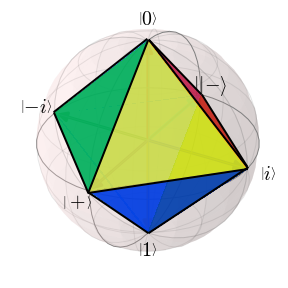
\includegraphics[width=.5\textwidth]{../Figures/Randomized benchmarking/Bloch sphere octahedron.png}
        \end{center}
        \caption{The single-qubit Clifford group can be visualized using an octahedron whose vertices correspond to the six cardinal states. The 24 Cliffords composing the single-qubit Clifford group correspond to the 24 distinct rotations of the octahedron such that the vertices are mapped onto themselves.}
        \label{fig:Clifford octahedron}
      \end{figure}

      The single qubit Pauli group consists of the two-dimensional identity operator and the three Pauli matrices. The $n$ qubit Pauli group is generated by the tensor product of $n$ single qubit Pauli groups. The $n$ qubit Clifford group $\mathpzc{C}_n$ is equal to the set of unitary transformations on the $n$ qubit Pauli group up to a global phase. The $n$ qubit Clifford group $\mathpzc{C}_n$ is generated by $\{H_i, P_i, CNOT_{ij}\} \forall i, j \in (1, \dots, n)$, where:

      \begin{equation}
        H =
        \frac{1}{\sqrt{2}}
        \begin{pmatrix}
          1 & 1 \\
          1 & 1
        \end{pmatrix}, \qquad
        P =
        \begin{pmatrix}
          1 & 0 \\
          0 & i
        \end{pmatrix}, \qquad
        CNOT =
        \begin{pmatrix}
          1 & 0 & 0 & 0 \\
          0 & 1 & 0 & 0 \\
          0 & 0 & 0 & 1 \\
          0 & 0 & 1 & 0
        \end{pmatrix}
      \end{equation}

      The single qubit Clifford group $\mathpzc{C}_1$ can be visualized using an octahedron in the Bloch sphere, as shown in Figure~\ref{fig:Clifford octahedron}. Each Clifford in $\mathpzc{C}_1$ corresponds to a distinct rotation of the octahedron, where the six cardinal states are mapped onto themselves. If one sets the constraint that the state $\ket{0}$ is mapped to itself, four distinct rotations are possible. Since the state $\ket{0}$ can be mapped to each of the six cardinal states, there are $6 \times 4=24$ distinct rotations, and hence $24$ Cliffords in the single qubit Clifford group $\mathpzc{C}_1$.

      Each of the Cliffords in the single qubit Clifford group $\mathpzc{C}_1$ can be decomposed into rotations along the X and Y axis, as is shown in Appendix~\ref{ssec:Clifford gate decomposition}. Each Clifford can be decomposed into a minimum of zero (identity) gates and a maximum of three gates. If one includes the identity as a gate, a Clifford requires on average 1.875 gates.

      The Clifford group does not form a universal set of gates. This is because the rotations only map cardinal states onto themselves. Since single qubit gates and CNOT is universal~\cite{nielsen2010quantum}, the Clifford group combined with the T-gate ($\pi/4$ rotation) constitute a set of universal quantum gates.

    \section{The randomized benchmarking protocol}
      \label{sec:randomized benchmarking protocol}

      \begin{wrapfigure}[7]{r}{0.4\textwidth}
        \begin{center}
        \vspace{-30pt}
          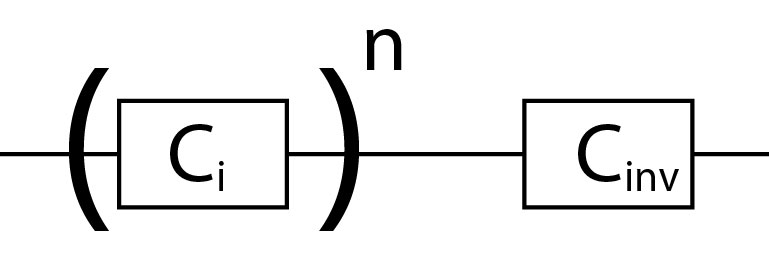
\includegraphics[width=.8\textwidth]{../Figures/Randomized benchmarking/RB schematic.jpg}
        \end{center}
        \vspace{-20 pt}
        \caption{Schematic of the randomized benchmarking protocol}
        \label{fig:RB schematic}
      \end{wrapfigure}

      Randomized benchmarking is a method to characterize the performance on qubits. It is based on repeated application of operations on the system, and measuring the fidelity to the ideal final state. The operations are randomly chosen from a set of unitary operations.

      In the case of the Muxmon experiment randomized benchmarking is performed on individual qubits, and the set of unitary operations is the single qubit Clifford group. The randomized benchmarking protocol used in this experiment, depicted in Figure~\ref{fig:RB schematic}, is as follows:

      \begin{enumerate}
        \item Initialize the qubit in the ground state
        \item Apply $n$ consecutive Cliffords $\left(C_1, \dots, C_n\right)$, where $C_i \in \mathpzc{C}_1 \; \forall \; i \in \left[1, \dots, n\right]$
        \item apply final inverting Clifford $C_\text{inv}=\left( C_n \dots C_1 \right)^{-1}$
        \item Measure the state of the qubit
      \end{enumerate}

      After the final inverting Clifford $C_\text{inv}$ the qubit should return to the ground-state. However, gate errors and decoherence result in the final state having a nonzero population in the excited-state. The final population in the ground-state $P_0$ decreases exponentially as the number of Cliffords $n$ is increased. In the limiting case where all information about the qubit is lost the qubit has equal population in the ground- and in the excited-state. The final ground-state population follows an exponential curve  given by~\cite{knill2008randomized}:

      \begin{equation}
        P_0= \frac{1}{2} p^n + \frac{1}{2}
        \label{eq:RB exponential decay}
      \end{equation}

      where $p$ is the decay parameter, related to the average fidelity per operation $F_0$ by~\cite{magesan2011scalable}:

      \begin{equation}
        F_o = \frac{1+p}{2}
      \end{equation}

      With knowledge of the average number of gates $n_g$ per operation, the average fidelity per operation can be translated to an average fidelity per gate $F_g$ via:

      \begin{equation}
        F_g = F_o^{1/n_g}
      \end{equation}

      Qubit relaxation places an upper limit on the number of gates that can be performed, and therefore on the fidelity per gate. This upper limit $F_\text{max}$ is given by:~\cite{knill2008randomized}:

      \begin{equation}
        F_\text{max} = \frac{1}{6}\left(3 + 2 e^{-t_g/2 T_1} + e^{-t_g/T_1}\right)
        \label{eq:RB T1 fidelity limit}
      \end{equation}

      where $t_g$ is the duration per gate, including any buffer between successive gates. As is expected this upper limit increases with shorter gates.

      \begin{figure}[tb]
        \centering
        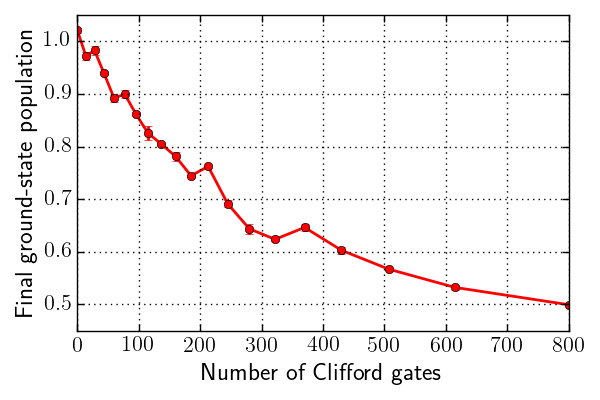
\includegraphics[width=.6\textwidth]{../Figures/Randomized benchmarking/RB_single_seed.png}
        \caption{Randomized benchmarking results using a single seed. The final ground-state population decreases exponentially as the number of Cliffords $n$ is increased. The points include errorbars, determined by the spread of three separate measurements.}
        \label{fig:RB single seed}
      \end{figure}

      To characterize the shape of the exponential decay in randomized benchmarking measurements, the successive values of $n$ in a measurement are separated by an exponentially increasing amount. Each set of random Cliffords is known as a seed. The randomized benchmarking results using a single seed are shown in Figure~\ref{fig:RB single seed}. Twenty points are chosen between $n=0$ and $n=800$ Clifford operations. As can be seen there is a clear exponential decay, in agreement with Formula~\ref{eq:RB exponential decay}. However, upon closer inspection the curve does not have a perfect exponential shape. This deviation is not due to insufficient averaging, but due to the fact that the Cliffords do not all have the same number of gates. A Clifford is on average composed of $1.875$ gates, but may be composed of anywhere between $1$ and $3$ gates. The result is that in a single seed some segments contain on average more than $1.875$ gates per Clifford, while other contain less. For a fixed error per gate, this results in fidelities deviating from the fidelity corresponding to exactly $1.875$ gates per Clifford. To obtain an accurate estimate for the exponential decay rate, multiple seeds must be used to average out the random fluctuations from the average gate per Clifford.

    \section{Single qubit randomized benchmarking}
      \label{sec:Single qubit randomized benchmarking}
      \subsection{Driving a single qubit versus driving both qubits}
        \label{ssec:Driving a single qubit versus driving both qubits}

        \begin{figure}[tb]
          \centering
          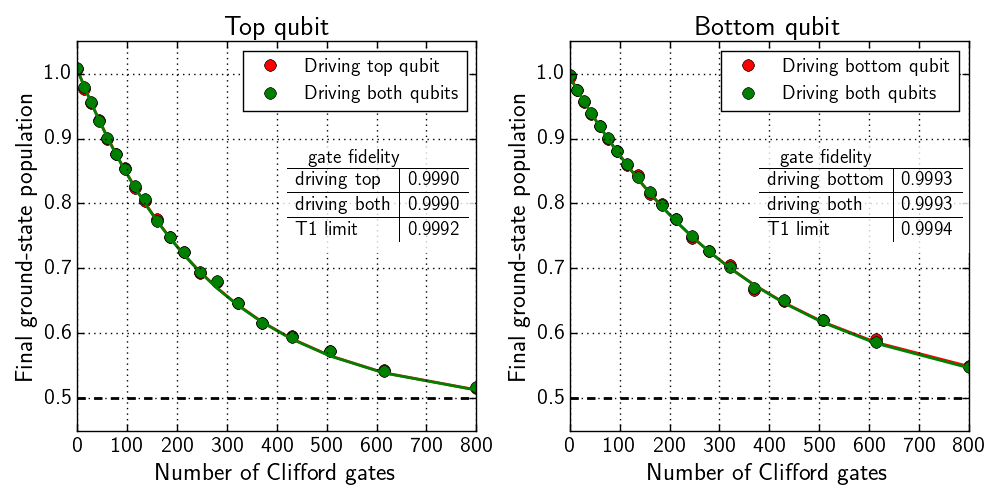
\includegraphics[width=\textwidth]{../Figures/Randomized benchmarking/RB_normal_driving_single_both.png}
          \caption{Randomized benchmarking results when driving a single qubit versus driving both qubits simultaneously. As can be seen there is no noticeable difference between driving only one qubit versus driving both qubits simultaneously. A total of 50 different seeds were used. T1 limits are calculated using Equation~\ref{eq:RB T1 fidelity limit}.}
          \label{fig:RB normal single vs both}
        \end{figure}

        After tuning up the top and bottom qubit using the calibration methods explained in Chapter~\ref{ch:Calibration routines}, their performance was determined using randomized benchmarking. To test whether the performance of the qubits change when driving only a single qubit or when simultaneously driving both qubits using the Duplexer, randomized benchmarking was performed in both cases. A total of 50 seeds were used for randomized benchmarking. For each seed $20$ different number of Cliffords $n$ are used, varying between $n=0$ and $n=800$, with exponentially separated points. Re-calibration of the drive amplitude and top qubit frequency was performed every 5 seeds to correct for small fluctuations in time. Pulses of \SI{16}{\nano \second} were used, with \SI{4}{\nano \second} buffer between pulses. For $800$ Cliffords this corresponds to a total duration of \SI{30}{\micro \second}.

        The randomized benchmarking results when driving only a single qubit or when driving both qubits simultaneously are shown in Figure~\ref{fig:RB normal single vs both}. As the number of Cliffords is increased, the ground-state population exponentially approaches the limiting value of $0.5$. The performance of both qubits reaches $99.9\%$ gate fidelity, and the performance of the bottom qubit is considerably better than that of the top qubit.  This can be expected, as the relaxation time and the dephasing time of the top qubit ($T_1 = \SIm{8.7}{\micro \second}$, $T_2^*=\SIm{4.7}{\micro \second}$) is lower than that of the bottom qubit ($T_1 = \SIm{11.1}{\micro \second}$, $T_2^*=\SIm{12.5}{\micro \second}$). Nevertheless, the gate fidelities of both qubits are still close to the limit imposed by $T_1$ (see Figure~\ref{fig:RB normal single vs both}). This shows that the qubit performance is mainly limited by its decoherence times, and not by the instruments including the AWG and Duplexer.

        \begin{figure}[tb]
          \centering
          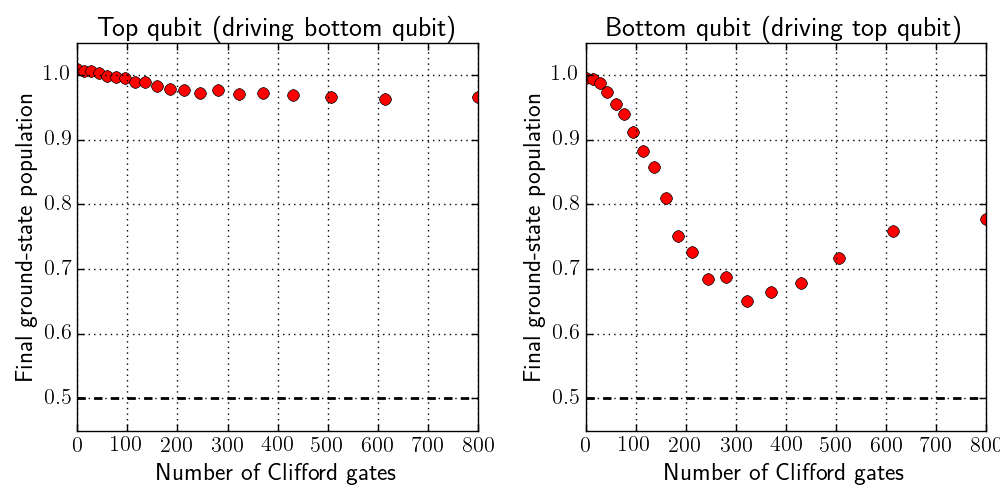
\includegraphics[width=\textwidth]{../Figures/Randomized benchmarking/RB_normal_cross-driving.png}
          \caption{Excitation in qubit when only the other qubit is driven during randomized benchmarking. This effect is mostly due to cross-driving and is considerably stronger for the top qubit than for the bottom qubit.}
          \label{fig:RB normal cross-driving}
        \end{figure}

        In Figure~\ref{fig:RB normal single vs both} it can furthermore be seen that there is no discernible difference in qubit performance between driving a single qubit and driving both qubits simultaneously. This indicates that cross-driving and cross-coupling effects do not affect the qubit performance during randomized benchmarking. One would expect that the measured cross-driving would place a lower bound on the qubit gate error ($0.57\%$ when driving the bottom qubit via the top qubit drive line, and $0.23\%$ when driving the top qubit via the bottom qubit drive line). However this does not seem to be the case. One possible explanation is that the transmon is a nonlinear system, and since the cross-driving measurements were performed at a high power, the cross-driving at low power might be significantly less.

        Figure~\ref{fig:RB normal cross-driving} shows the ground-state population during randomized benchmarking when only the other qubit is driven. This should ideally be unity irrespective of the number of Cliffords applied, but one can see that application of pulses on one qubit also affects the state of the qubit not being driven. The excitation of the qubit not being driven may be due to cross-coupling, or due to cross-driving, or a combination of the two effects. This effect is much stronger when driving the top qubit and measuring the bottom qubit than the other way around. This is in agreement with the cross-driving measurements in Section~\ref{sec:cross-driving}, inidicating that the effect is mainly due to cross-driving, and not cross-coupling. Furthermore, the period of the excitation swap was previously found to be equal to $J^{-1} \approx \SIm{14}{\micro \second}$, whereas the duration of the longest pulse sequence, corresponding to $n=800$ Cliffords, is equl to \SI{30}{\micro \second}. Cross-coupling effects should not depend on which qubit is being driven, and so the fact that the top qubit is not excited much, even after $n=800$ Cliffords, places an upper bound on the cross-coupling effects. This further supports the claim that the main source of the undriven qubit's excitation is due to cross-driving.

      \subsection{Second-state leakage}
        \label{ssec:Second-state leakage}
        The exponential fits to the single qubit randomized benchmarking measurements show that the asymptote of the exponential curve actually lies slightly below a ground-state population of $0.5$. This is in contrast to expectation, as in the limiting case in randomized benchmarking, where all information about the qubit is lost, a measurement of the qubit should result in the qubit being foud with equal probability in the ground-state and in the excited-state. One possible explanation for this deviation from $0.5$ is that during the randomized benchmarking sequence the qubit experiences leakage to the second excited-state, which would shift the measured signal.

        To test whether the exponential curve not saturating at $0.5$ is indeed due to leakage, an identical randomized benchmarking measurement set has been performed using the same $50$ seeds. At the end of each Clifford sequence a final pi pulse is applied. The result is that the final ground-state and excited-state populations are swapped. In this case the final state should therefore ideally be the excited-state.

        If we assume there is no further leakage into states higher than the second-state, these two measurements result in the following set of equations:

        \begin{align}
          p_0 V_0 + p_1 V_1 + p_2 V_2 = S_0 \notag\\
          p_1 V_1 + p_0 V_1 + p_2 V_2 = S_1 \notag\\
          p_0 + p_1 + p_2 = 1
          \label{eq:three populations equations}
        \end{align}

        where $p_i$ is the final population of state $\ket{i}$, $V_i$ is the measured signal corresponding to state $\ket{i}$, and $S_i$ is the signal measured for a fixed number of Cliffords $n$ where the qubit's final state should ideally by $\ket{i}$. If the signals corresponding to all three states are known, the three populations can be extracted (see Appendix~\ref{ssec:Determining population in three states} for details).

        \begin{figure}[tb]
          \centering
          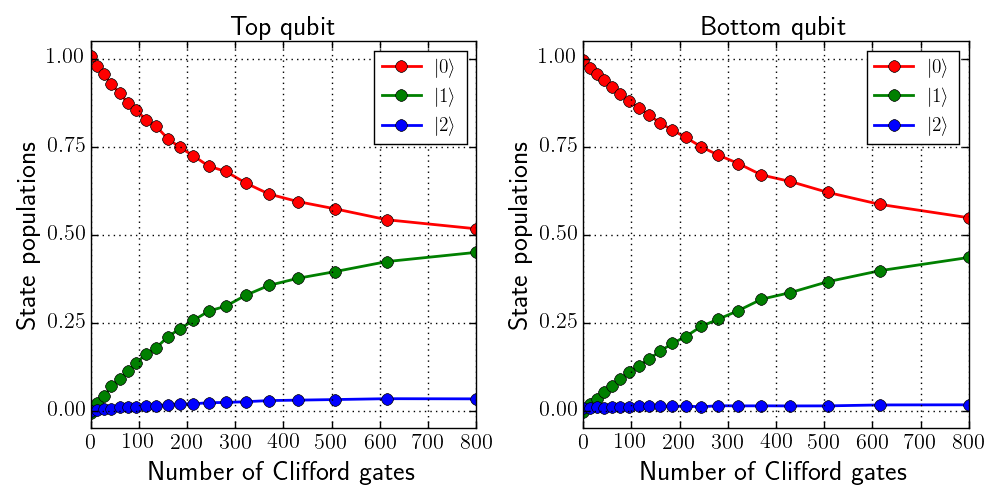
\includegraphics[width=\textwidth]{../Figures/Randomized benchmarking/RB_normal_state_populations.png}
          \caption{The populations of the first three states of the qubit during randomized benchmarking. Populations are extracted by comparing randomized benchmakring results with and without a final pi pulse (see Appendix~\ref{ssec:Determining population in three states}). As can be seen, both qubits suffer from a small amount of leakage to the second-state. The leakage rate for the top qubit is higher than for the bottom qubit.}
          \label{fig:RB normal state populations}
        \end{figure}

        Using the methods explained in Section~\ref{ssec:Second-state}, the signal $V_2$ of the second-state has been measured and added as a calibration point to the randomized benchmarking sequence. With knowledge of the signals corresponding to all three states, the populations of the first three states of the qubits during randomized benchmarking have been determined. The results are shown in Figure~\ref{fig:RB normal state populations}. As can be seen there is indeed a small amount of leakage present. The leakage rate is higher for the top qubit than for the bottom qubit. Increasing the pulse length would result in a smaller frequency bandwidth, and is therefore expected to lower the leakage rate. This has, however, not yet been tested.

        \begin{itemize}
          \item Mention that drag can be optimized for leakage, although this would result in a higher gate error. Must find paper
        \end{itemize}

    \section{Two qubit randomized benchmarking}
      \label{Two qubit randomized benchmarking}
      So far randomized benchmarking on two qubits has only been performed in the case where both qubits receive the same pulses. In a more realistic scenario one would like to be able to control both qubits individually. The Duplexer, in combination with frequency re-use, offers this possibility. The switches of the Duplexer are able to route pulses at nanosecond-scale. Using a single sequence of pulses, these switches allow each individual pulse to be sent to either of the two qubits, or both qubits simultaneously. This is known as selective broadcasting, and enables individual control of both qubits simultaneously.

      The performance of controlling both qubits simultaneously using selective broadcasting has been studied using randomized benchmarking. In this case each of the two qubits has an individual seed composed of $n$ randomly chosen Cliffords. There are many different ways in which randomized benchmarking on two qubits can be performed. Three methods have been explored: alternating randomized benchmarking, compiled randomized benchmarking, and 5 primitives randomized benchmarking. These will be explained in the following sections.

      \begin{itemize}
        \item Additionally since the qubits are driven by the same pulses, their states should be identical.
      \end{itemize}

      \subsection{Alternating randomized benchmarking}
        \label{ssec:alternating randomized benchmarking}

        \begin{figure}[tb]
          \centering
          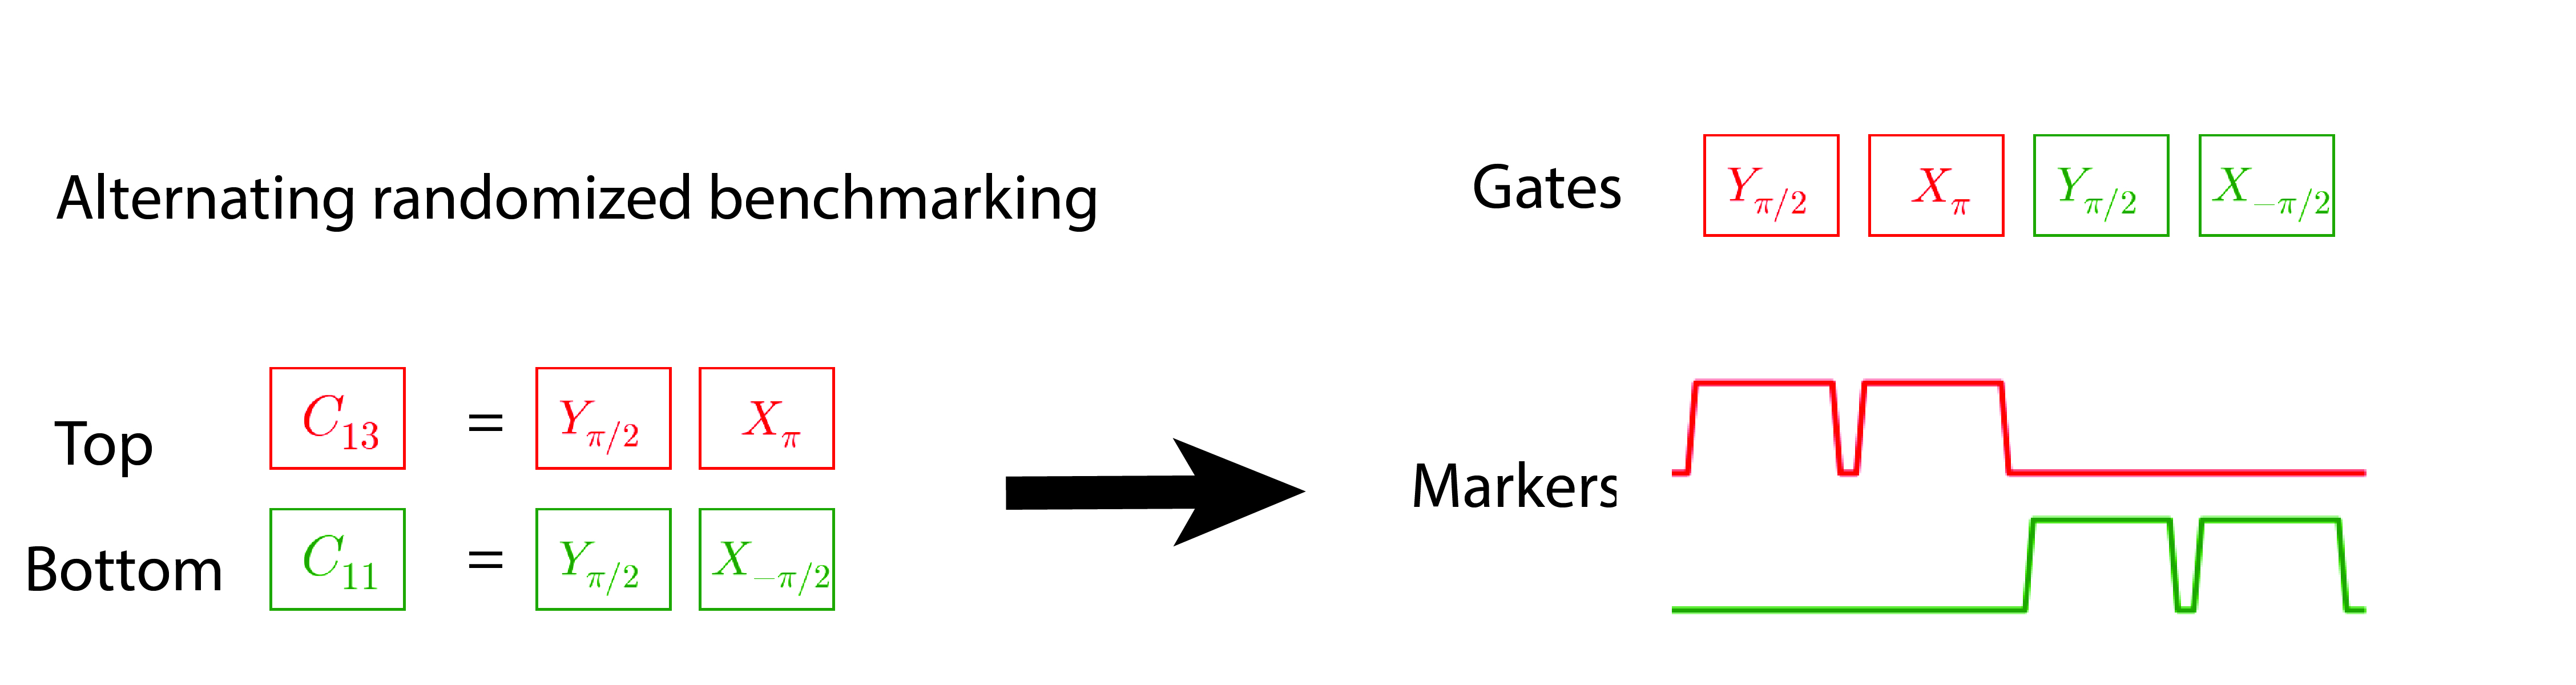
\includegraphics[width=\textwidth]{../Figures/Randomized benchmarking/alternating RB.jpg}
          \caption{Alternating randomized benchmarking}
          \label{fig:alternating RB schematic}
        \end{figure}

        The first method explored is alternating randomized benchmarking. In this method the Cliffords of the two qubits are applied alternatingly, as shown in Figure~\ref{fig:alternating RB schematic}. When a Clifford of the top qubit is applied, the switches of the top qubit are on, while the switches of the bottom qubit are off, and vice versa. If each qubit has a seed composed of $n$ Cliffords, the total duration of the sequence will be twice as long as in single qubit randomized benchmarking. Therefore the average duration of a pair of Clifford is equal to $2 \times 1.875 = 3.75$ gates.


      \subsection{Compiled randomized benchmarking}
        \label{ssec:compiled randomized benchmarking}

        \begin{figure}[tb]
          \centering
          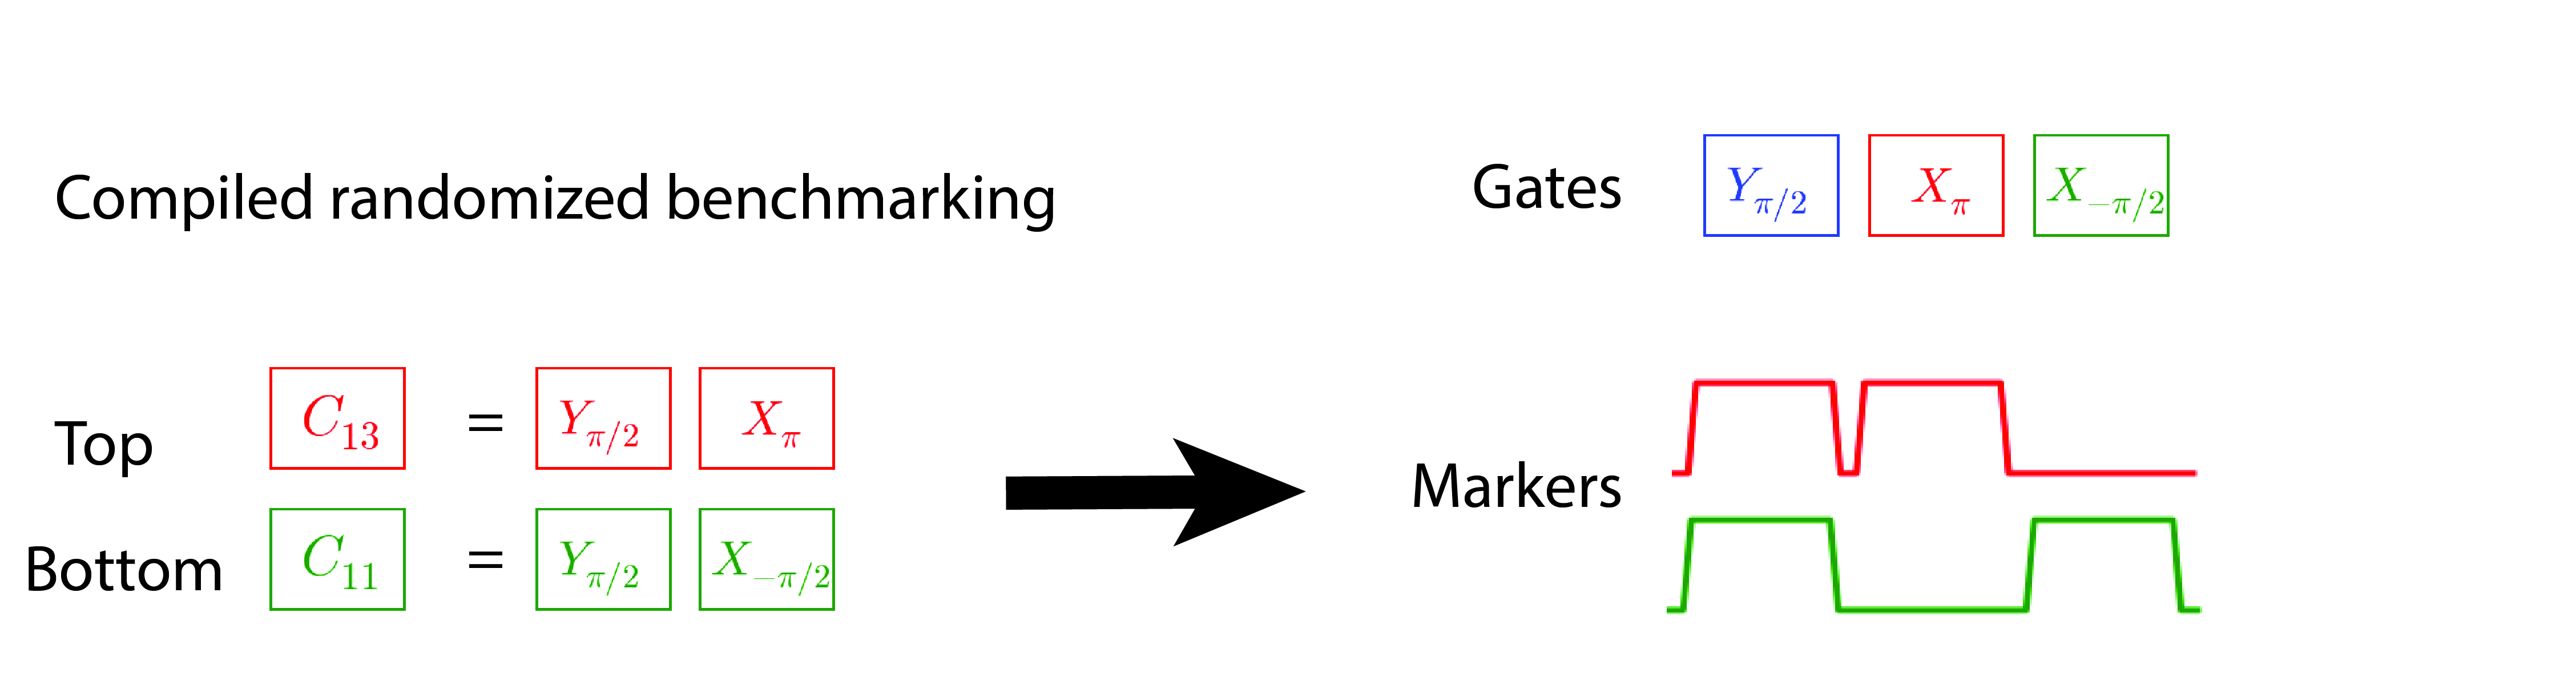
\includegraphics[width=\textwidth]{../Figures/Randomized benchmarking/compiled RB.jpg}
          \caption{Compiled randomized benchmarking}
          \label{fig:compiled RB schematic}
        \end{figure}

        In alternating randomized benchmarking pulses are never simultaneously applied to both qubits. However, it is quite possible that a pair of Cliffords has one or more gates in common. Compiled randomized benchmarking is a more efficient alternative to alternating randomized benchmarking, where pairs of Cliffords are compiled into the least amount of physical gates required to perform both Cliffords. The schematic is shown in Figure~\ref{fig:compiled RB schematic}, where the same Clifford combination is shown as in the schematic of alternating randomized benchmarking (Figure~\ref{fig:alternating RB schematic}). As can be seen both Clifford decompositions share the $Y_{\pi/2}$ gate, and so can be combined into a single pulse sent to both qubits simultaneously. The result is that the total number of gates is reduced from four to three.

        Compiled randomized benchmarking even goes one step further. The Clifford decomposition shown in Appendix~\ref{fig:Clifford decomposition} is one way in which the $24$ Cliffords can be decomposed. There are, however, many other possible decompositions for each of the Cliffords into rotations along the X and Y axis. It is not at all obvious which decompositions of the two Cliffords would result in the optimal gate compilation for a given Clifford pair, i.e. the least amount of physical gates required to perform the pair of Cliffords on the two qubits.

        If we ignore decompositions where successive gates cancel, such as $X_{\pi/2}$, followed by $X_{-\pi/2}$, and only look at decompositions up to $4$ gates, there are $903$ possible combinations of gates, resulting in an average of approximately $38$ possible decompositions per Clifford. This corresponds to $38^2=1444$ possible pairs of decompositions. In compiled randomized benchmarking the optimal compilation from all these possible decomposition pairs is found. (see Appendix~\ref{sec:compiled randomized benchmarking algorithm} for details on the algorithm used). The result of this compilation is that on average the duration of a pair of Cliffords is equal to $2.925$ gates, which is $22\%$ less than alternating randomized benchmarking ($3.75$ gates per Clifford pair).

      \subsection{5 primitives randomized benchmarking}
        \label{ssec:5 primitives randomized benchmarking}

        \begin{figure}[tb]
          \centering
          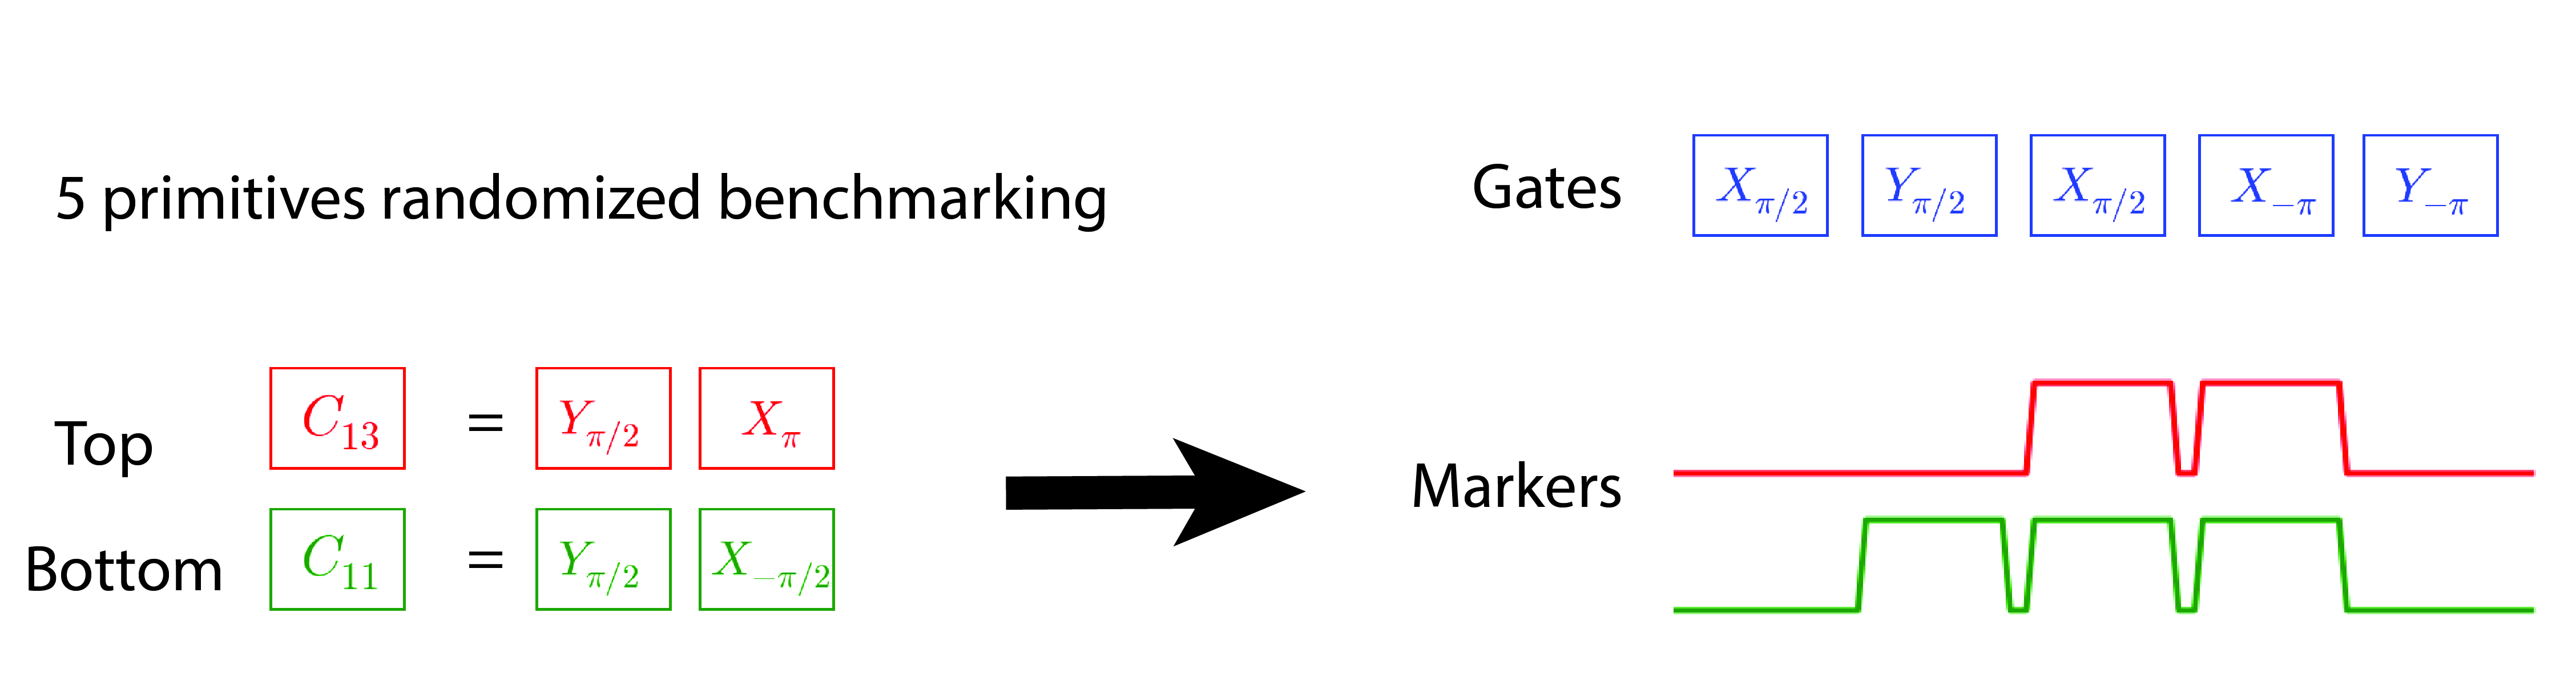
\includegraphics[width=\textwidth]{../Figures/Randomized benchmarking/5 primitives RB.jpg}
          \caption{5 primitives randomized benchmarking}
          \label{fig:5 primitives RB schematic}
        \end{figure}

        When exploring different two qubit randomized benchmarking methods, one very interesting property of the Clifford group was discovered. It was found that each of the $24$ Cliffords can be decomposed into a subset of $5$ primitive gates, while retaining the gate order of the $5$ primitives. The $5$ primitive gates are:

        \begin{figure}[h!]
          \centering
          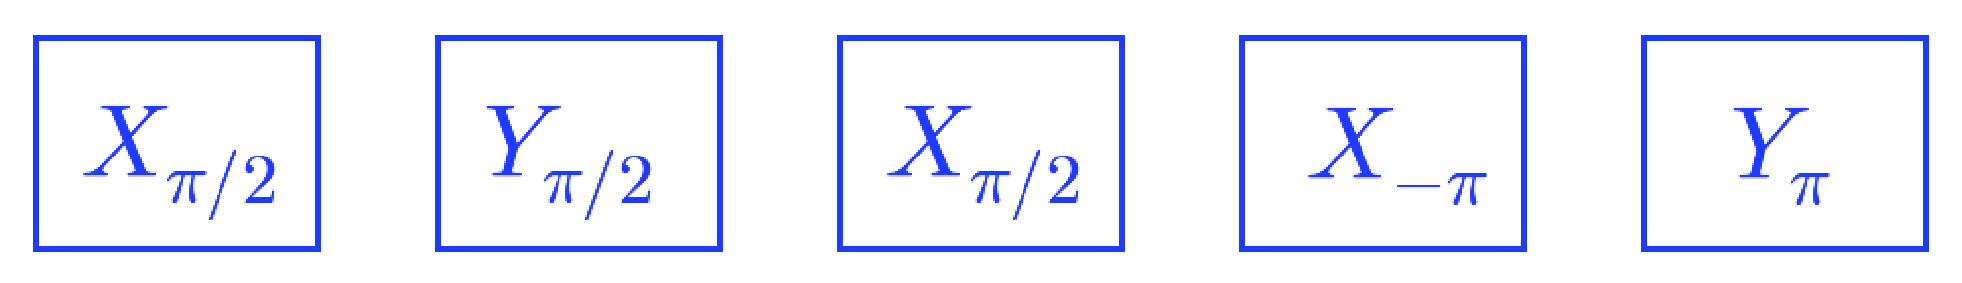
\includegraphics[width=.5\textwidth]{../Figures/Randomized benchmarking/5 primitive gates.jpg}
          \caption{The 5 primitive gates, in order of application in time.}
          \label{5 primitive gates}
        \end{figure}

        Using the fixed set of $5$ primitive gates, and by selectively routing the pulses to each of the qubits, arbitrary Cliffords can simultaneously be applied both qubits. The Cliffords applied to the two qubits need not be equal. In the $5$ primitives method the gate sequence stays fixed, and could even be continuously repeated. The markers corresponding to the state of the switches determine the Clifford operations of the qubits.

        There is another advantage of the $5$ primitive gates, which is that it decreases the amount of cross-driving when one of the two qubits is not being driven. The first three gates composing the $5$ primitives are positive $\pi/2$ gates along the X and Y axes. The final two gates are negative $\pi$ gates along the X and Y axes. Cross-driving corresponds to rotations where the angle is a fraction of the full rotation angle. After one full $5$ primitive gates cycle the state of the idle qubit should therefore return close to its initial position. Even if not all $5$ gates are applied, the cross-driving effects should still decrease. This is because the cross-driving rotations are small, and in randomized benchmarking a large number of random Cliffords are applied, and so over the course of an entire randomized benchmarking run these cross-driving effects will still partially cancel out.

        An even better approach to eliminating cross-driving is to alternate between a cycle of the $5$ primitive gates, and a cycle where the $5$ primitive gates are inverted, i.e. negative $\pi/2$ rotations and positive $\pi$ rotations, and switching of the gate order. Since the Clifford set is a group, each Clifford has a unique inverse which is also a Clifford. Inverting a Clifford is equal to inverting the gates of its $5$ primitives decomposition (including reversal of the gate order). Since all the inverted gates are elements of the inverted $5$ primitive gates, we see that we can indeed also decompose all $24$ Cliffords using the inverted $5$ primitive gates. Alternating between the $5$ primitive gates and the inverted $5$ primitive gates is expected to reduce the effects of cross-driving even further, as any deviation from returning to the original position in the first $5$ primitives cycle is compensated for by the inverted cycle.

        The $5$ primitives randomized benchmarking method alternates between the $5$ primitives cycle and the inverted $5$ primitives cycle. The $5$ primitives randomized benchmarking requires $5$ gates per Clifford pair, which is considerably more than compiled randomized benchmarking ($2.925$ gates per Clifford pair) and alternating randomized benchmarking ($3.75$ gates per Clifford pair).

        \section{Two qubit randomized benchmarking results}
          \label{Two qubit randomized benchmarking results}

          \begin{figure}[tb]
            \centering
            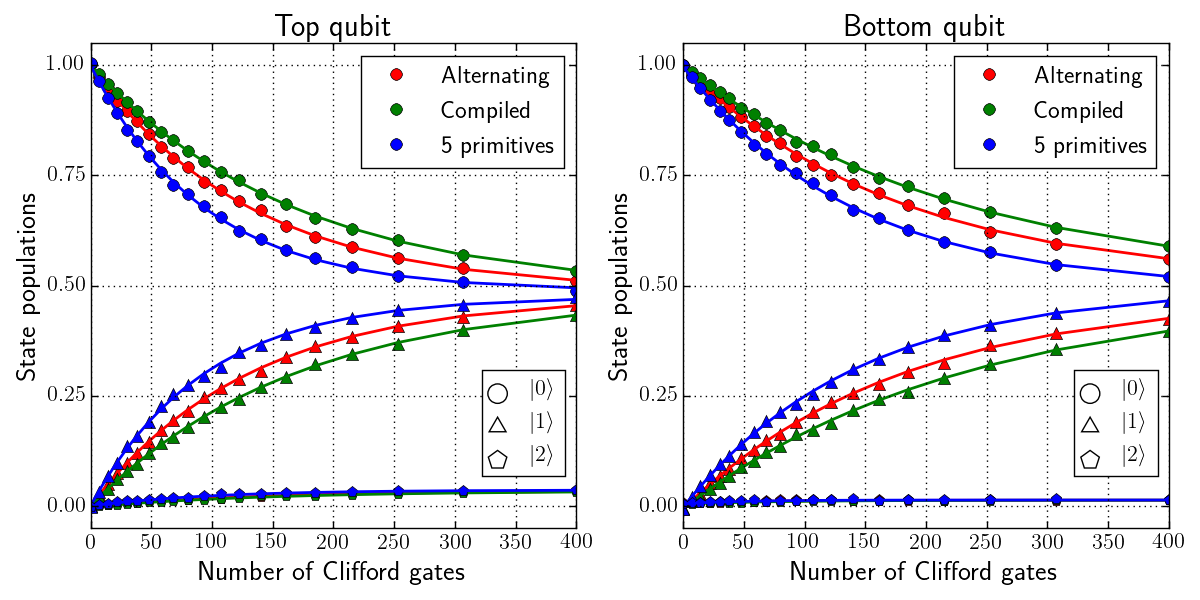
\includegraphics[width=\textwidth]{../Figures/Randomized benchmarking/RB_2Q_state_populations_notable.png}
            \caption{State populations using three different two qubit randomized benchmarking sequences. Number of Cliffords correspond to each qubit. A total of $50$ seeds was used. The measurements were performed with and without a final pi pulse, from which the populations of the first thee states of the qubit were determined.}
            \label{fig:RB 2Q state populations}
          \end{figure}

      \begin{table}
        \begin{tabular}{l c c c c}
          \toprule
          RB method     & \multicolumn{2}{c}{Clifford fidelity} & \multicolumn{2}{c}{gate fidelity}\\
          \cmidrule(lr){2-3}
          \cmidrule(lr){4-5}
                        & top qubit & bottom qubit & top qubit & bottom qubit \\
          \midrule
          Alternating   & 0.9962 & 0.9972 & 0.9990 & 0.9992 \\
          Compiled      & 0.9970 & 0.9978 & 0.9990 & 0.9992 \\
          5 primitives  & 0.9947 & 0.9964 & 0.9990 & 0.9993 \\
          \bottomrule
        \end{tabular}
        \caption{Corresponding gate fidelities of top and bottom qubit using three randomized benchmarking methods. The gate fidelities are obtained using the corresponding average gates per Clifford.}
        \label{tab:RB 2Q converted gate fidelities}
      \end{table}

          The three different two qubit randomized benchmarking methods have been performed for a total of $50$ seeds. Up to $n=400$ Cliffords per qubit were used, and the pulse length was kept at \SI{16}{\nano \second} with a \SI{4}{\nano \second} buffer between pulses. By performing the measurements both with and without a final pi pulse, the populations of the first three states of the qubit have been determined (see Appendix~\ref{ssec:Determining population in three states}). The results are shown in Figure~\ref{fig:RB 2Q state populations}. For all three methods the bottom qubit performs considerably better than the top qubit, which is expected considering the decoherence times of the qubits. For both qubits compiled randomized benchmarking has the lowest error per Clifford, after which alternating randomized benchmarking, while $5$ primitives randomized benchmarking has the highest error per Clifford. This is in agreement with the average gates per Clifford, which is smallest for compiled Randomized benchmarking, and largest for $5$ primitives randomized benchmarking. Nevertheless we see that for both qubits all three methods result in fidelities per Clifford exceeding $99\%$. The fidelity per Clifford can be converted to a corresponding fidelity per gate using the average gates per Cliffords of the three methods. The corresponding gate fidelities are shown in Table~\ref{tab:RB 2Q converted gate fidelities}. As can be seen the gate fidelities are nearly identical, and furthermore are equal to the single qubit randomized benchmarking gate fidelities. This comparison is not entirely fair, as idle gates (when only the other qubit is being pulsed) are also counted as gates. Nevertheless, it can be concluded that there is no significant decrease in gate fidelity when using selective broadcasting. These results show that simultaneous control of two qubits can be achieved with an error rate below the single qubit suface code fault tolerant threshold.

          \begin{figure}[tb]
            \centering
            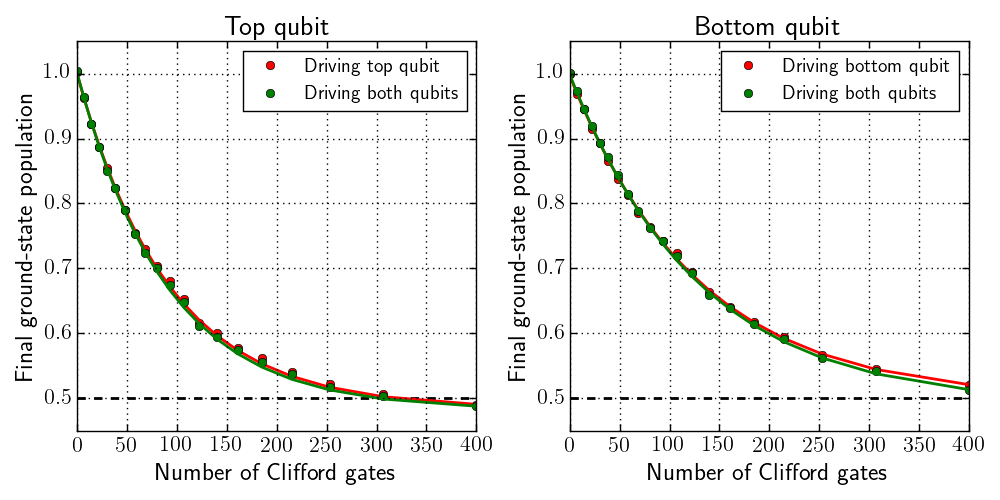
\includegraphics[width=\textwidth]{../Figures/Randomized benchmarking/RB_5p_driving_single_both.png}
            \caption{$5$ primitives randomized benchmarking results when driving a single qubit versus driving both qubits simultaneously. A total of 50 different seeds were used.}
            \label{fig:RB 5P single vs both}
          \end{figure}

          In Figure~\ref{fig:RB 5P single vs both} the effect of driving a single qubit versus driving both qubits simultaneously is shown using $5$ primitives randomized benchmarking. As can be seen there is no noticeable change in qubit performance.

          \begin{figure}[tb]
            \centering
            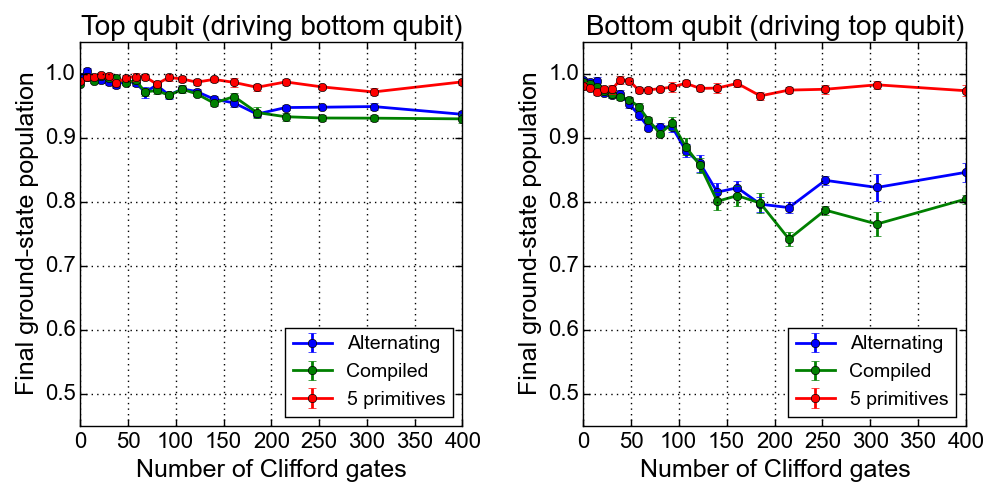
\includegraphics[width=\textwidth]{../Figures/Randomized benchmarking/RB_2Q_driving_single_vs_both.png}
            \caption{Excitation in qubit when only the other qubit is driven during randomized benchmarking. This effect is mostly due to cross-driving and is considerably stronger for the top qubit than for the bottom qubit. A total of $5$ seeds was used}
            \label{fig:cross driving two qubit randomized benchmarking}
          \end{figure}

          In Figure~\ref{fig:cross driving two qubit randomized benchmarking} we can see the effect of cross-driving during two qubit randomized benchmarking. In this case the switches corresponding to one qubit are continuously closed, while the other qubit is being driven. As can be seen the bottom qubit experiences much more cross-driving than the top qubit. We see, however, that this cross-driving is greatly reduced when using the $5$ primitives method. This is due to the fact that the pulses in the $5$ primitives method are chosen such that the cross-driving effects for idle qubits are reduced (see Section~\ref{ssec:5 primitives randomized benchmarking}).

        \section{Scaling of multi qubit randomized benchmarking}
          \label{sec:scaling of multi qubit randomized benchmarking}

          \begin{figure}[tb]
            \centering
            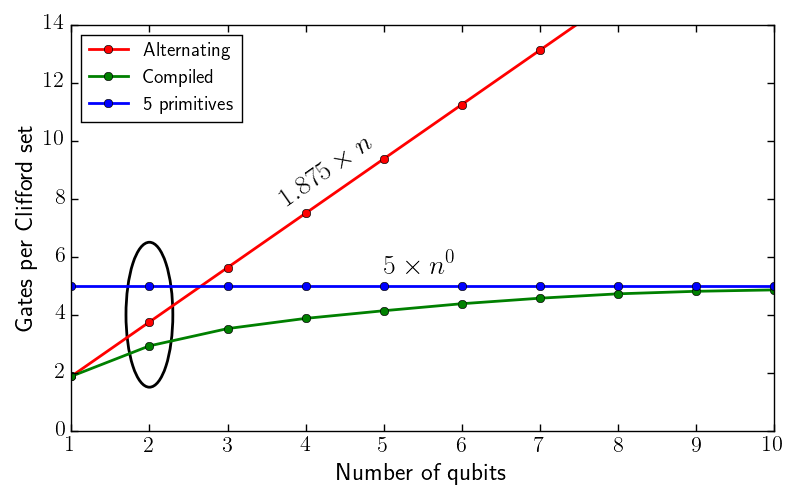
\includegraphics[width=.8\textwidth]{../Figures/Randomized benchmarking/Clifford_comparison.png}
            \caption{Comparison of the average gates per Clifford set versus the number of qubits using the three different multi qubit randomized benchmarking methods. The oval indicates the gates per Clifford at two qubits}
            \label{fig:gate per Clifford versus qubits comparison}
          \end{figure}

          So far it has been found that for two qubits compiled randomized benchmarking clearly performs best, while $5$ primitives method performs worst. The performance is directly related to the average number of gates per Clifford set. Figure~\ref{fig:gate per Clifford versus qubits comparison} shows how the average number of gates per Clifford scale a function of the number of qubits for all three randomized benchmarking methods. At two qubits the $5$ primitives method performs worst of all three methods. However, at three qubits the $5$ primitives method already outperforms alternating randomized benchmarking. This is because the $5$ primitives method has $5$ gates per Clifford, irrespective of the number of qubits, whereas alternating randomized benchmarking scales linearly with the number of qubits.

          Compiled randomized benchmarking always performs the best, as it per definition finds the least amount of gates required to perform a set of Cliffords on the qubits. However, compiled randomized benchmarking has a clear disadvantage, which is that the required time for finding the optimal compilation scales exponentially with the number of qubits. Each Clifford on average has $38$ different decompositions, and so for five qubits this would already result in $38^5\approx 7.9 * 10^{7}$ different combinations for each individual set of Cliffords. Furthermore, finding the average gates per Clifford requires knowledge of the gates per Clifford for all different combinations of Cliffords, and so for five qubits this would result in $6.3*10^{14}$ different combinations of decompositions. Using several optimization methods, which are discussed in Appendix~\ref{Optimizing the gate compilation algorithm}, the average gates per Clifford has been determined exactly for up to five qubits, and approximated up to ten qubits using random sampling. Nevertheless it is still computationally intensive to find the optimal gate compilation, even for a modest amount of qubits.

          In contrast to the compiled randomized benchmarking method, the $5$ primitives randomized benchmarking method is computationally very easy to perform. Once a marker lookup table has been created (see Appendix~\ref{ssec:Clifford gate decomposition}), determining the $5$ primitives decomposition of an arbitrary number of Cliffords is simply a matter of looking up the corresponding marker sequences. Furthermore, at $5$ qubits the difference in average gates per Clifford between the compiled randomized benchmarking and the $5$ primitives randomized benchmarking is already less than $1$, and so unless the number of qubits is small, the $5$ primitives randomized benchmarking is the best and by far easiest of the three randomized benchmarking methods.


  \chapter{Conclusions and outlook}

    When the top and bottom qubit are tuned to the same frequency, cross-coupling and cross-driving effects do become noticeable. This could potentially be a problem, as it results in correlated errors. The fact that the cross-driving effects in the Muxmon1 experiment are stronger than in the Muxmon0 device suggest that they dependent on the amount of components separating same-frequency qubits. The same holds for cross-coupling effects. Therefore, if it turns out that in the surface code architecture these effects must be reduced, a modified frequency re-use structure could be implemented. For instance, by using a total of eight frequencies instead of four, qubits sharing the same frequency can be separated by more components, thereby reducing these adverse effects.

    When the top and bottom qubit share the same frequency, it has been shown that they can be simultaneously controlled by a single generator in combination with the Duplexer. Through randomized benchmarking it has been shown that for both qubits the gate fidelity reaches $99.9$ per cent, thereby meeting the surface code fault-tolerant threshold. The gate fidelity is within a factor of two of limit imposed by its relaxation time $T_1$, indicating that the qubit performance is in fact decoherence limited.

    It has furthermore been shown that there is no change in performance when driving a single qubit versus driving both qubits simultaneously. It is interesting to note that the gate fidelities exceed the maximum one would expect considering the cross-driving measured. One possible explanation is that the cross-driving measurements were performed at high power, and since the transmon is a nonlinear system, it is possible that the cross-driving is lower at low drive powers.

    Furthermore, it has been shown individual control of both qubits simultaneously is possible through selective broadcasting. This has been demonstrated using multi-qubit randomized benchmarking, where each qubit has a different seed. Three different multi-qubit randomized benchmarking schemes have been implemented, namely alternating, compiled, and $5$ primitives randomized benchmarking. It has been shown for all three methods the Clifford fidelity exceeds $99$ per cent, thereby also meeting the surface code fault-tolerant threshold. Converting the Clifford fidelities to gate fidelities using their average gates per Clifford it has shown to be identical to the gate fidelities obtained by single qubit randomized benchmarking, showing that there is no significant decrease in performance when using selective broadcasting.

    Of the three multi-qubit randomized benchmarking methods, alternating randomized benchmarking clearly scales the worst with number of qubits. Compiled randomized benchmarking per definition always scales the best. However, the complexity of finding the optimal gate compilation scales exponentially, making it a highly non-trivial challenge. The $5$ primitives randomized benchmarking, remains fixed at $5$ gates per Clifford, irrespective of the number of qubits. In contrast to the compiled randomized benchmarking however, finding the Clifford decomposition using the $5$ primitives method can be done using a simple lookup table. furthermore, the average gates per Clifford using compiled randomized benchmarking converges to $5$ quite rapidly, and so unless the number of qubits is small, the gain using compiled randomized benchmarking is small.

    When randomized benchmarking is only performed on one of the qubits, while the other at the same frequency remains idle, cross-driving effects have been observed. However, it has been shown in the $5$ primitives method that by cleverly choosing pulses, cross-driving effects when the other qubit is idle can largely be corrected.

    During the randomized benchmarking sequences leakage to the second excited-state has been observed. The leakage rate is found to be worse for the top qubit than for the bottom qubit. The DRAG parameter has a different optimum value for correcting phase error than it has for minimizing leakage. Since it has been calibrated to minimize the phase error, changing the DRAG parameter could therefore potentially reduce leakage, although this would result in more phase error during gates. Additionally, leakage could be reduced by resorting to longer pulses.

    Even though the Duplexer already proves to be very useful in a measurement set-up, it is only the first step in a path aimed at reducing the amount of intstruments. The next generation Duplexer is already being made, which will be a true multiplexer having a variable number of outputs. This will be a huge step in the road to scaling up.

    There is one additional advantage of the $5$ primitives method, which is that the $5$ primitive gate sequence remains fixed. Therefore it is not needed to generate qubit pulses on demand, but only to control the qubit switch. This could potentially have an application in a quantum processor, where a central pulse generator continuously repeats the same $5$ pulses. By selectively directing the pulses to each of the qubits using a switch matrix, each qubit could have access to any given Clifford at any time. The consequence is that for single-qubit Clifford gates the pulses do not need to be generated on demand, but can simply be continuously looped. The timing of the switches is the only thing that needs to be directed, which is a far easier challenge. If the $5$ primitive gates are combined with a sixth gate, such as the T-gate, this would even result in any universal single-qubit gates being accessible to any qubit, simply through control of its corresponding switch.  This technique could even possibly be extended to two-qubit gates, where the flux pulses could be similarly controlled. This would mean that a universal set of quantum gates could be generated for qubits by only controlling the corresponding switches. It might even be extended to qubit readout, as the readout tonescould be directed via switching as well.

    Having continuously streaming pulses, which are directed to the qubits via selective broadcasting could have ... consequences, as this would shift the challenge from generating pulses when required to only controlling the switches. This would have important consequences. First of all the feedback response time could improve significantly. Furthermore the amount of data required to be sent into the fridge could be reduced significantly. However, the most important consequence is probably that the amount of instruments required would be reduced significantly, potentially even reaching a constant as the number of qubits grow. This might prove to be an important step in the pathway to building a quantum computer.